%%%%%%%%%%%%%%%%%%%%%%% file template.tex %%%%%%%%%%%%%%%%%%%%%%%%%
%
% This is a general template file for the LaTeX package SVJour3
% for Springer journals.          Springer Heidelberg 2010/09/16
%
% Copy it to a new file with a new name and use it as the basis
% for your article. Delete % signs as needed.
%
% This template includes a few options for different layouts and
% content for various journals. Please consult a previous issue of
% your journal as needed.
%
%%%%%%%%%%%%%%%%%%%%%%%%%%%%%%%%%%%%%%%%%%%%%%%%%%%%%%%%%%%%%%%%%%%
%
% First comes an example EPS file -- just ignore it and
% proceed on the \documentclass line
% your LaTeX will extract the file if required
%
\RequirePackage{fix-cm}
%
%\documentclass{svjour3}                     % onecolumn (standard format)
%\documentclass[smallcondensed]{svjour3}     % onecolumn (ditto)
\documentclass[smallextended]{svjour3}       % onecolumn (second format)
%\documentclass[twocolumn]{svjour3}          % twocolumn
%
\smartqed  % flush right qed marks, e.g. at end of proof
%
\usepackage{graphicx}
%
% \usepackage{mathptmx}      % use Times fonts if available on your TeX system
%
% insert here the call for the packages your document requires
%\usepackage{latexsym}
% etc.
%
% please place your own definitions here and don't use \def but
% \newcommand{}{}
%
% Insert the name of "your journal" with
 \journalname{Statistical Papers}
%

\spnewtheorem{assumption}{Assumption}{\bf}{\it}

\usepackage{galois} % composition function \comp
\usepackage{bm}
\usepackage{amsmath}
\usepackage{amssymb}
\usepackage{mathrsfs}
%\usepackage[numbers]{natbib}
\usepackage{natbib}
\usepackage{graphicx}
\usepackage{color}
\usepackage{booktabs}
\usepackage[page,title]{appendix}
%\renewcommand\appendixname{haha}
\usepackage{enumerate}
\usepackage{changepage}
\usepackage{datetime}
\usepackage[FIGTOPCAP]{subfigure}
%\newdate{date}{9}{1}{2017}

%%%%%%%%%%%%%%  Notations %%%%%%%%%%
\DeclareMathOperator{\mytr}{tr}
\DeclareMathOperator{\mydiag}{diag}
\DeclareMathOperator{\myRank}{Rank}
\DeclareMathOperator{\myP}{P}
\DeclareMathOperator{\myE}{E}
\DeclareMathOperator{\myVar}{Var}
\DeclareMathOperator{\myCov}{Cov}
\DeclareMathOperator*{\argmax}{arg\,max}
\DeclareMathOperator*{\argmin}{arg\,min}


\newcommand{\Ba}{\mathbf{a}}    \newcommand{\Bb}{\mathbf{b}}    \newcommand{\Bc}{\mathbf{c}}    \newcommand{\Bd}{\mathbf{d}}    \newcommand{\Be}{\mathbf{e}}    \newcommand{\Bf}{\mathbf{f}}    \newcommand{\Bg}{\mathbf{g}}    \newcommand{\Bh}{\mathbf{h}}    \newcommand{\Bi}{\mathbf{i}}    \newcommand{\Bj}{\mathbf{j}}    \newcommand{\Bk}{\mathbf{k}}    \newcommand{\Bl}{\mathbf{l}}
\newcommand{\Bm}{\mathbf{m}}    \newcommand{\Bn}{\mathbf{n}}    \newcommand{\Bo}{\mathbf{o}}    \newcommand{\Bp}{\mathbf{p}}    \newcommand{\Bq}{\mathbf{q}}    \newcommand{\Br}{\mathbf{r}}    \newcommand{\Bs}{\mathbf{s}}    \newcommand{\Bt}{\mathbf{t}}    \newcommand{\Bu}{\mathbf{u}}    \newcommand{\Bv}{\mathbf{v}}    \newcommand{\Bw}{\mathbf{w}}    \newcommand{\Bx}{\mathbf{x}}
\newcommand{\By}{\mathbf{y}}    \newcommand{\Bz}{\mathbf{z}}    
\newcommand{\BA}{\mathbf{A}}    \newcommand{\BB}{\mathbf{B}}    \newcommand{\BC}{\mathbf{C}}    \newcommand{\BD}{\mathbf{D}}    \newcommand{\BE}{\mathbf{E}}    \newcommand{\BF}{\mathbf{F}}    \newcommand{\BG}{\mathbf{G}}    \newcommand{\BH}{\mathbf{H}}    \newcommand{\BI}{\mathbf{I}}    \newcommand{\BJ}{\mathbf{J}}    \newcommand{\BK}{\mathbf{K}}    \newcommand{\BL}{\mathbf{L}}
\newcommand{\BM}{\mathbf{M}}    \newcommand{\BN}{\mathbf{N}}    \newcommand{\BO}{\mathbf{O}}    \newcommand{\BP}{\mathbf{P}}    \newcommand{\BQ}{\mathbf{Q}}    \newcommand{\BR}{\mathbf{R}}    \newcommand{\BS}{\mathbf{S}}    \newcommand{\BT}{\mathbf{T}}    \newcommand{\BU}{\mathbf{U}}    \newcommand{\BV}{\mathbf{V}}    \newcommand{\BW}{\mathbf{W}}    \newcommand{\BX}{\mathbf{X}}
\newcommand{\BY}{\mathbf{Y}}    \newcommand{\BZ}{\mathbf{Z}}    

\newcommand{\bfsym}[1]{\ensuremath{\boldsymbol{#1}}}

 \def\balpha{\bfsym \alpha}
 \def\bbeta{\bfsym \beta}
 \def\bgamma{\bfsym \gamma}             \def\bGamma{\bfsym \Gamma}
 \def\bdelta{\bfsym {\delta}}           \def\bDelta {\bfsym {\Delta}}
 \def\bfeta{\bfsym {\eta}}              \def\bfEta {\bfsym {\Eta}}
 \def\bmu{\bfsym {\mu}}                 \def\bMu {\bfsym {\Mu}}
 \def\bnu{\bfsym {\nu}}
 \def\btheta{\bfsym {\theta}}           \def\bTheta {\bfsym {\Theta}}
 \def\beps{\bfsym \varepsilon}          \def\bepsilon{\bfsym \epsilon}
 \def\bsigma{\bfsym \sigma}             \def\bSigma{\bfsym \Sigma}
 \def\blambda {\bfsym {\lambda}}        \def\bLambda {\bfsym {\Lambda}}
 \def\bomega {\bfsym {\omega}}          \def\bOmega {\bfsym {\Omega}}
 \def\brho   {\bfsym {\rho}}
 \def\btau{\bfsym {\tau}}
 \def\bxi{\bfsym {\xi}}
 \def\bzeta{\bfsym {\zeta}}



\begin{document}

\title{
A Bayesian-motivated test for high-dimensional linear regression models with fixed design matrix
%\thanks{Grants or other notes
%about the article that should go on the front page should be
%placed here. General acknowledgments should be placed at the end of the article.}
}
%\subtitle{Do you have a subtitle?\\ If so, write it here}

\titlerunning{High-dimensional linear model}        % if too long for running head

\author{ Rui Wang         \and
        Xingzhong Xu %etc.
}

%\authorrunning{Short form of author list} % if too long for running head

\institute{Rui Wang \at
School of Mathematics and Statistics, Beijing Institute of Technology, Beijing 100081, China
              %\email{fauthor@example.com}           %  \\
%             \emph{Present address:} of F. Author  %  if needed
           \and
           Xingzhong Xu \at
School of Mathematics and Statistics, Beijing Institute of Technology, Beijing 100081, China
\\
and
\\
Beijing Key Laboratory on MCAACI, Beijing Institute of Technology, Beijing 100081,China
\\
\email{xuxz@bit.edu.cn}           %  \\
}

\date{Received: date / Accepted: date}
% The correct dates will be entered by the editor


\maketitle

\begin{abstract}

This paper considers testing regression coefficients in high-dimensional linear model with fixed design matrix.
    We prove that there does not exist nontrivial unbiased test for this problem.
    %This phenomenon makes it impossible to consider the problem from a minimax perspective.
    Moreover, no test can guarantee nontrivial power even when the true model is largely deviate from the null hypothesis.
    Nevertheless, Bayesian methods can still produce tests with good average power behavior.
    We propose a new test statistic which is the limit of Bayes factors under normal distribution.
    The null distribution of the proposed test statistic is approximated by Lindeberg's replacement trick.
    Under certain conditions, the global asymptotic power function of the proposed test is also given.
    The finite sample performance of the proposed test is demonstrated via simulation studies.
\keywords{Fixed design matrix \and High-dimensional test \and Lindeberg method \and Linear model \and Unbiasedness }
% \PACS{PACS code1 \and PACS code2 \and more}
 \subclass{62H15 \and 62J05 }
\end{abstract}


\section{Introduction} 
Consider linear regression model of the form
\begin{equation}\label{label:linearModel}
    \By = 
    \BX_a \bbeta_a + \BX_b \bbeta_b + \bepsilon, %\quad \bepsilon\sim \mathcal N_n(0,\phi^{-1} \BI_n),
\end{equation}
where $\By \in \mathbb R^n$ is the response, $\BX_a$, $\BX_b$ are $n\times q$ and $n\times p$ design matrices, respectively,  $\bbeta_a\in \mathbb R^q$, $\bbeta_b\in \mathbb R^p$ are unknown regression coefficients, and 
$\bepsilon\in \mathbb R^n$ is the vector of random errors.
Here the design matrix $\BX_a$ contains the predictors that are known to have effects on the response,
and our interest is to test if $\BX_b$ contains any useful predictors.
That is, we would like to test the hypotheses
\begin{align}\label{theHypothesis}
    \mathcal H_0:   \bbeta_b =0,\quad
    \text{v.s.} \quad
    \mathcal H_1:   \bbeta_b \neq 0.
\end{align}
%Motivated by many recent applications of high-dimensional regression, we consider the situation where $p+q$ is much larger than $n$.
The conventional test for hypotheses \eqref{theHypothesis} is the $F$-test which is also the likelihood ratio test under normal errors.
However, the $F$-test is not well defined in high-dimensional setting.
In fact, if $\bepsilon$ is normal distributed and $\myRank[\BX_a;\BX_b]=n$, then the likelihood is unbounded under the alternative hypothesis.
Thus, new test methodology is required in high-dimensional setting.

For the problem of testing hypotheses \eqref{theHypothesis}, two different high-dimensional settings have been extensively considered in the literature.
One is the small $p$, large $q$ setting.
An important example of this setting is testing individual coefficients of a high-dimensional regression.
See \cite{buhlmann2013statistical,Zhang2013,Lan2016} for testing procedures in this setting.
In this paper, however, we focus on the other setting, namely the large $p$, small $q$ setting.
In this case, there are just a few covariates, namely $\BX_a$, are known to have effects on the response, while there remain a large number of covariates, namely $\BX_b$, to be tested.
%We assume $\BX_a$ has full column rank and $\BX_b$ has full row rank.
%In practice, which covariates belong to the part $\BX_a$ is determined apriori.
%If no prior knowledge is available, $\BX_a$ can be $\mathbf 1_n$.
%In both cases, $q$ is often relatively small.
%However, there may remain a very large number of variables in $\BX_b$, so $p>n$.

Many test procedures have been proposed in the large $p$, small $q$ setting.
Based on an empirical Bayes model, \cite{Goeman2006} and \cite{Goeman2011} proposed a score test statistic as well as a method to determine the critical value.
This score test was further investigated by \cite{Lan2014Testing} and \cite{Lan2016a}.
Based on $U$-statistics, \cite{Zhong2011Tests} proposed a test for the case where $\BX_a=\mathbf 1_n$.
Their method was then extended and improved by \cite{Wang2015} and \cite{Cui2018}, respectively.
%Wang and Cui \cite{Wang2015} extended the test of Zhong and Chen \cite{Zhong2011Tests} to the case where $\BX_a$ is a general design matrix.
To accommodate outlying observations and heavy-tailed distributions, \cite{Feng2013}
proposed a rank-based test for the entire coefficients.
\cite{Xu2016a} modified the test of \cite{Feng2013} and proposed a scalar invariant rank-based test.
\cite{Janson2016} utilized a convex optimization program to obtain an unbiased estimator of a signal to noise ratio with small variance, based on which a test is constructed.
Apart from the aforementioned tests,
there is another line of research utilizing desparsified Lasso estimator; see, e.g., \cite{Dezeure2017} \cite{ZC2017}.

Most existing high-dimensional tests adopted the random design assumption, that is, the rows of $\BX_b$ are considered as being generated from a super population.
Often in practice, however, at least a part of the design matrix is designed by the experimenter; see \cite{Draper1996} and the references therein.
In this case, assuming a random design is not appropriate.
Hence in this paper, we consider the fixed design setting.
Of course, our test method is still valid for random design from a conditional inference perspective.
As noted by \cite{Lei2018}, assuming a fixed design or a random design could lead to qualitatively different inferential results.
%In fact, the fixed design setting is much more irregular than the random design setting.
In frequentist hypotheses testing,
unbiasedness and minimaxity are two important considerations of test methods; see, e.g., \cite{Lehmann}.
Under the random design assumption, nontrivial unbiased test does exist and the testing problem can be considered from the minimax perspective; see, e.g., \cite{ITV2010}.
Surprisingly, these two frequentist considerations can not be applied in the fixed design setting.
In fact, in Section \ref{sec:unbiased}, we shall show that in the fixed design setting, the only unbiased test and minimax test is the trivial constant function $\varphi(\By) \equiv \alpha$.
This negative result of frequentist considerations motivates us to propose a frequentist test with the aid of Bayesian methods.

In this paper, we propose a new test statistic for hypotheses \eqref{theHypothesis} which is the limit of Bayes factors as the prior magnitude of $\bbeta_b$ tend to infinity.
The proposed test statistic is a ratio of quadratic forms of $\By$.
We give an approximation of the distribution of quadratic form using Lindeberg's replacement trick.
Based on this approximated distribution, the critical value of the proposed test statisitc is calculated by a one step iteration.
We prove that the proposed test procedure is valid under weak conditions.
In particular, the validity of the proposed test procedure does not require that the test statistic is asymptotically normally distributed.
The proposed test statistic is closely related to the test statistic of \cite{Goeman2006} which is also derived by a Bayesian argument.
However, \cite{Goeman2006} let the prior magnitude of $\bbeta_b$ tend to zero, which is contrary to our strategy.
Under certain conditions, we derive the asymptotic power function of the proposed test and the test of \cite{Goeman2006}.
It is shown that the proposed test can detect the signals from more directions than the test of \cite{Goeman2006}.

%In fact, the test procedure of \cite{Goeman2006} is motivated by Bayesian methods but is treated as a frequentist test.
%But this work will use a different strategy to set prior magnitude.
%In \cite{Goeman2006}, the prior distribution of $\bbeta_b$ satisfies $\myE (\bbeta_b)= 0$, $\myVar (\bbeta_b)=c \BI_p$ and their statistic is obtained by letting $c$, the prior magnitude of $\bbeta_b$, tend to zero.
%Their goal is to achieve the highest average power under local alternative.
%In classical statistics, any reasonable test can detect large deviations from the null hypothesis and it is natural to consider only the local alternative.
%Surprisingly, though, the situation is different for our problem.
%In fact, Theorem \ref{prop:unbiased} will show that no test can detect all large deviations from the null hypothesis in large $p$, small $q$ setting.
%Consequently, it is not enough to consider only the local alternative.
%Simulations are conducted to examine the good performance of the proposed test.

This paper has made three main contributions for testing hypotheses \eqref{theHypothesis} in large $p$, small $q$ setting with fixed design matrix.
First, we prove that no test can detect all large deviations from the null hypothesis.
Second, we propose a novel Bayesian-motivated test, which can be regarded as an extention of the likelihood ratio test in high-dimensional setting.
Third, we propose to use Lindeberg's replacement trick to approximate the distribution of quadratic forms.

The rest of the paper is organized as follows.
In Section \ref{sec:unbiased}, we prove the nonexistence of unbiased test for hypotheses \eqref{theHypothesis} in large $p$, small $q$ setting.
In Section \ref{sec:methodology}, we propose a Bayesian-motivated test and study the theoretical properties of the proposed test procedure.
The asymptotic power function is also derived.
Section \ref{sec:Numerical} contains the simulation results. 
Section \ref{sec:conclusions} concludes the paper.
The technical proofs are presented in Appendix.


\section{Nonexistence of unbiased test}\label{sec:unbiased}

In this paper, we consider testing hypotheses \eqref{theHypothesis} in large $p$, small $q$ setting.
More specifically, we make the following assumption throughout the paper.
\begin{assumption}
    In the linear model \eqref{label:linearModel}, 
    suppose $\bepsilon=(\epsilon_1,\ldots,\epsilon_n)^\top$ where $\epsilon_1,\ldots, \epsilon_n$ are independent indentically distributed (iid) with $\myE (\epsilon_1) = 0$ and $\myVar (\epsilon_1) = \phi^{-1}$.
    Furthermore, suppose $q<n$, $\myRank(\BX_a)=q$ and $\myRank([\BX_a; \BX_b])=n$.
    \label{Assumption}
\end{assumption}
%Based on an empirical Bayes model,
%\cite{Goeman2006} and \cite{Goeman2011} proposed a score test which can be used.
Testing hypotheses \eqref{theHypothesis} in large $p$, small $q$ setting is a challenging problem.
\cite{Goeman2006} noticed that their test has negligible power for many alternatives and consequently is not an unbiased test.
Biased tests are often regarded as problematic in classical statistics.
However, the situation is very different for our problem.
In fact, we shall show that under normal assumption, there is no nontrivial unbiased test in large $p$, small $q$ setting.

Let $\BP_a=\BX_a(\BX_a^\top \BX_a)^{-1} \BX_a^\top$ be the projection matrix onto the column space of $\BX_a$ and denote $\tilde \BP_a = \BI_n-\BP_a$.
Define $\btheta =(\bbeta_a^\top , \bbeta_b^\top , \phi)^\top$ and 
\begin{equation*}
    \begin{split}
        &\Theta_0 = \left\{\btheta=(\bbeta_a^\top , \bbeta_b^\top , \phi)^\top: \bbeta_a \in \mathbb R^{q}, \bbeta_b=0, \phi>0\right\},
    \\
    &\Theta = \left\{\btheta=(\bbeta_a^\top , \bbeta_b^\top , \phi)^\top: \bbeta_a \in \mathbb R^{q}, \bbeta_b\in \mathbb R^p, \phi>0\right\}.
    \end{split}
\end{equation*}
A test function $\varphi(\By)$ of level $\alpha$ is a Borel measurable function from $\mathbb R^n$ to $\mathbb R$ such that $0\leq \varphi(\By) \leq 1$ and $\myE_{\btheta} [\varphi(\By)]\leq \alpha$ for $\btheta\in \Theta_0$.
Let $\lambda(\cdot)$ be the Lebesgue measure on $\mathbb R^n$.
We have the following theorem.
\begin{theorem}\label{prop:unbiased}
    Suppose Assumption \ref{Assumption} holds.
    Furthermore, assume $\bepsilon\sim \mathcal N_n (0, \phi^{-1}\BI_n)$.
    Let $\varphi(\By)$ be a test function of level $\alpha$, $0 <\alpha <1$.
    If $\lambda(\{\By:\varphi(\By)\neq \alpha\})>0$, then for every $M\geq 0$, there exists a parameter $\btheta=(\bbeta_a^\top,\bbeta_b^\top,\phi)^\top \in \Theta$ such that $\phi\bbeta_b^\top \BX_b^\top \tilde \BP_a \BX_b \bbeta_b > M$ and $\myE_{\btheta} [\varphi(\By)]< \alpha$.
\end{theorem}
In Theorem \ref{prop:unbiased}, the quantity $\phi \bbeta_b^\top \BX_b^\top \tilde \BP_a \BX_b \bbeta_b$ can be regarded as a signal to noise ratio.
In any conventional sense, it is expected that the power of a reasonable test should tend to $1$ as $\phi \bbeta_b^\top \BX_b^\top \tilde \BP_a \BX_b \bbeta_b \to \infty$.
Indeed, such a test can be easily constructed in low dimensional setting.
However, Theorem \ref{prop:unbiased} claims that it is impossible to find such a test in large $p$, small $q$ setting.
Moreover, Theorem \ref{prop:unbiased} implies that the trivial test $\varphi(\By) \equiv \alpha$ (a.e.\ $\lambda$) is the only unbiased test and is also the only minimax test for testing $\mathcal H_0 $ against $\mathcal H_1^{M}: \phi\bbeta_b^\top \BX_b^\top \tilde \BP_a \BX_b \bbeta_b > M$ for any $M > 0$.
This is somewhat surprising since nontrivial unbiased test and minimax test do exist in random design setting; see, e.g., \cite{ITV2010}.

Note that unbiasedness and minimaxity are two key considerations of frequentist hypotheses testing; see, e.g., \cite{Lehmann}.
In our problem, however, these considerations can not be applied and there is no test with guaranteed power.
Nevertheless, it is still feasible to propose a test with good average power behavior.
Note that from the viewpoint of the decision theory, Bayesian methods aim at minimizing the average risk; see, e.g., \cite{Lehmann}, Section 1.6.
This motivates us to propose a frequentist test with the aid of Bayesian methods.
%Then Bayesian methods are natural choices for our porpuse.
%This motivates us to consider tests with good average power behavior.
%Hence and classical frequentist strategies for constructing tests may not be suitable.
%Classical strategies for constructing tests may not be suitable since there is no nontrivial unbiased test nor test with guaranteed power.



\section{A Bayesian-motivated test}\label{sec:methodology}

In Bayesian literature, Bayes factor (see, e.g., \cite{Robert1995Bayes}) is a fundamental tool for hypotheses testing and model comparison.
So far, many Bayesian tests have been proposed for hypothesis \eqref{theHypothesis} in low-dimensional setting; see \cite{javier2006Obj,Goddard2016,zhou2018On} and the references therein.
However, most existing Bayesian tests are not applicable in large $p$, small $q$ setting.
In this section, we shall propose a new frequentist test statistic in large $p$, small $q$ setting which is the limit of Bayesian factors.
In principle, using Bayes factor as a frequentist test statistic in high-dimensional setting is a good strategy for at least two reasons.
First, the Bayes factors corresponding to proper priors are always well defined, even if the likelihood is unbounded.
Second, under mild conditions, tests based on Bayes factors are admissible (See, e.g., \cite{Lehmann}, Theorem 6.7.2).

\subsection{Test statistic}
The new test statistic will be derived under normal assumption.
%We assume in the derivation of the test statistic.
Later we will show that the proposed test method can be applied for general distribution.
Suppose $\bepsilon \sim \mathcal N_n (0,\phi^{-1} \BI_n)$, then the Bayes factor for hypotheses \eqref{theHypothesis} is
\begin{equation*}
    B_{10}= \frac {
        \int d\mathcal N_n(\BX_a\bbeta_a + \BX_b\bbeta_b, \phi^{-1}\BI_n) (\By) \pi_1(\bbeta_b,\bbeta_a,\phi)\, \mathrm d\bbeta_b \mathrm d\bbeta_a \mathrm d\phi
}{
    \int d\mathcal N_n(\BX_a\bbeta_a, \phi^{-1} \BI_n)(\By) \pi_0(\bbeta_a,\phi) \, \mathrm d\bbeta_a \mathrm d\phi
    },
\end{equation*}
where $d\mathcal N_n(\mu, \bSigma)(\By)$ is the density function of a $\mathcal N_n(\mu,\bSigma) $ random vector evaluated at $\By$,  $\pi_0(\bbeta_a,\phi)$ and $\pi_1(\bbeta_b,\bbeta_a,\phi)$ are the prior densities under the null and alternative hypotheses, respectively.
If $B_{10}$ is large, the alternative hypothesis is preferred.
%There have been several extensions of $g$-priors to $p>n$ case: \cite{maruyama2011}, \cite{Shang2011}.
It is known that if the true parameters indeed come from the specified prior distribution, then the Bayes factor is the likelihood ratio statistic and consequently, the test based on the Bayes factor is the most powerful test.
We notice that in the frequentist framework, the Bayes factor can be treated as a test statisitc provided the critical value can be determined to preserve the test level.
%It is known that the test based on Bayes factor is admissible, namely, its the power can not be uniformly dominated by any other test.


The behavior of a Bayes factor largely depends on the choice of priors.
In Bayesian literature, many priors have been considered for testing the coefficients of linear model.
Popular priors include $g$-priors \citep{Liang2008Mixtures} and intrinsic priors \citep{Casella2006Obj}.
Unfortunately, these priors are not well defined in large $p$, small $q$ setting.
%To obtain valid Bayes factor, we use simple priors.
Note that under the null hypothesis $\mathcal H_0$, the model is low-dimensional.
This allows us to impose the reference prior $\pi_0 (\bbeta_a,\phi)=c/\phi$, where $c$ is a constant.
Under $\mathcal H_1$,
write $\pi_1(\bbeta_b,\bbeta_a,\phi)=\pi_1(\bbeta_b|\bbeta_a,\phi) \pi_1(\bbeta_a,\phi)$.
For parameters $\bbeta_a $ and $\phi$, we consider the same prior as in $\mathcal H_0$, that is $\pi_1(\bbeta_a,\phi)=\pi_0(\bbeta_a,\phi)$.
For parameter $\bbeta_b$, however, imposing the improper reference prior would not produce valid marginal density of $\By$.
%That is, the minimal training sample size is $q + p +1$.
%So we cannot impose the reference prior under $ H_1$ provided $q + p  \geq n$.
To make the marginal density of $\By$ well defined,
we consider the simple normal prior $p_1(\bbeta_b|\bbeta_a, \phi) = d \mathcal N_{p} (0, \kappa^{-1} \phi^{-1} \BI_{p}) (\bbeta_b) $, where $\kappa>0$ is a hyperparameter.
That is, we put the following priors,
\begin{equation}\label{priors}
    \pi_0(\bbeta_a,\phi)= \frac{c}{\phi},\quad
    \pi_1(\bbeta_b,\bbeta_a,\phi)=\frac{c}{\phi} d \mathcal N_{p} \left(0, \frac{1}{\kappa \phi} \BI_{p}\right) (\bbeta_b).
\end{equation}
%There are extansive literature consider the choice of $\kappa$.
%\cite{Kass1995} choose $\kappa$ such that the amount of information about the parameter equal to the amount of information contained in one observation.
%\begin{equation*}
    %\begin{split}
    %m_0(\By;\kappa, \tau) 
    %&:=
    %\int f_0^\tau (\By|\bbeta_a,\phi) \pi_0 (\bbeta_a, \phi) d\bbeta_a d\phi
    %\\
    %&=
    %\frac{
        %c_0 \Gamma\left( \frac{\tau n - q}{2}\right)
    %}{
        %\pi^{\frac{\tau n - q }{2}}
        %\tau^{\frac{\tau n}{2}}
        %|\BX_a^\top \BX_a|^{\frac{1}{2}}
        %\| (\BI_n -\BP_a) \By\|^{\tau n -q}
    %}.
    %\end{split}
%\end{equation*}
%\begin{equation*}
    %\begin{split}
        %m_1(\By;\kappa, \tau) 
    %&:=
    %\int f_1^\tau (\By|\bbeta_b,\bbeta_a,\phi) \pi_1 (\bbeta_b |\bbeta_a, \phi) \pi_1 (\bbeta_a, \phi)  d\bbeta_a d\bbeta_b d\phi
    %\\
    %&=
    %\frac{c_1\kappa^{\frac p 2} \Gamma \left(\frac{\tau n -q}{2}\right)}{
        %\pi^{\frac{\tau n -q}{ 2 }} \tau^{\frac{\tau n + p}{2}}
        %|\BX_a^\top \BX_a|^{\frac 1 2}
        %|\BX_b^{*\top} \BX_b^* + \frac{\kappa}{\tau } \BI_p|^{\frac 1 2}
    %}
    %\frac{1}{\left[ \By^{*\top} \By^* - \By^{*\top} \BX_b^* ( \BX_b^{*\top}\BX_b^* + \frac{\kappa}{\tau} \BI_p )^{-1} \BX_b^{*\top} \By^* \right]^{\frac{\tau n - q}{2}}}
    %.
    %\end{split}
%\end{equation*}
%\begin{equation*}
    %\begin{split}
        %\frac{m_1(\By;\kappa,\tau)}{m_0(\By;\kappa,\tau)} 
        %=
        %\frac{c_1 \kappa^{\frac{p}{2}}}{c_0 \tau^{\frac p 2}
        %|\BX_b^{*\top} \BX_b^* + \frac{\kappa}{\tau } \BI_p|^{\frac 1 2}
        %}
        %\left(
            %\frac{\By^{*\top} \By^*}{
%\By^{*\top} \By^* - \By^{*\top} \BX_b^* ( \BX_b^{*\top}\BX_b^* + \frac{\kappa}{\tau} \BI_p )^{-1} \BX_b^{*\top} \By^*
            %}
        %\right)^{\frac{\tau n - q }{2}}
    %\end{split}
%\end{equation*}

%In what follows, we assume $\myRank (\BX_a )=q$ and $\myRank ([\BX_a;\BX_b])=n$.
Let $B_{10,\kappa} $ be the Bayes factor corresponding to the priors \eqref{priors}.
 It is straightforward to show that
%\begin{equation*}
    %\begin{split}
        %B_{10,\kappa}=  &
    %\frac{\kappa^{p/2}}{
        %|\BX_b^\top (\BI_n -\BP_a) \BX_b + \kappa \BI_p |^{1/2}
    %}
    %\cdot
    %\\
    %&
    %\left(
        %\frac{
            %\By\top (\tilde \BP_a) \By
        %}{
            %\By\top (\tilde \BP_a) \By
            %-
            %\By\top (\tilde \BP_a) \BX_b
            %\left(\BX_b^\top  (\BI-\BP_a) \BX_b + \kappa \BI_p\right)^{-1}
            %\BX_b^\top (\tilde \BP_a) \By
        %}
    %\right)^{(n-q)/2}.
    %\end{split}
%\end{equation*}
 \begin{equation}\label{new:tuoyan1}
    \begin{split}
        &2\log (B_{10,{\kappa}})
        \\
        =  &
    p\log \kappa
    -
        \log |\BX_b^\top \tilde \BP_a \BX_b + \kappa \BI_p |
    \\
    &
    -(n-q)\log \left(
            1-
        \frac{
            \By^\top \tilde \BP_a \BX_b
            \left(\BX_b^\top  \tilde \BP_a \BX_b + \kappa \BI_p\right)^{-1}
            \BX_b^\top \tilde \BP_a \By
        }{
            \By^\top \tilde \BP_a \By
        }
    \right).
    \end{split}
\end{equation}

Denote by $\tilde \BP_a=\tilde{\BU}_a \tilde{\BU}_a^\top$ the rank decomposition of $\tilde \BP_a$, where $\tilde{\BU}_a$ is an $n\times (n-q)$ column orthogonal matrix.
Let $\BX_b^* = \tilde{\BU}_a^\top \BX_b$, $\By^* =\tilde \BU_a^\top \By$.
Let $\gamma_i$ be the $i$th largest eigenvalue of $\BX^*_b \BX_b^{*\top}$, $i=1,\ldots, n-q$.
Denote by $\BX_b^* =\BU_{b}^* \BD_{b}^* \BV_b^{*\top}$ the singular value decomposition of $\BX_{b}^*$, where  $\BU_{b}^*$, $\BV_b^*$ are $(n-q)\times (n-q)$ and $p\times (n-q)$ column orthogonal matrices, respectively, and $\BD_{b}^*=\mydiag (\sqrt {\gamma_1},\ldots, \sqrt{\gamma_{n-q}})$.
Then we have
\begin{equation*}
    \begin{split}
        &2\log (B_{10,\kappa})
        \\
        %=&
         %p\log \kappa
         %- \sum_{i=1}^{n-q}\log ( \gamma_i + \kappa )
         %-(p-(n-q))\log \kappa
         %\\
         %&-(n-q)\log\left(1-\frac{\By^{*\top} \BX_b^* \left( \BX_b^{*\top} \BX_b^* + \kappa \BI_p \right)^{-1} \BX_b^{*\top} \By^* }{\By^{*\top} \By^*}\right)
         %\\
        %=&
         %- \sum_{i=1}^{n-q}\log ( \gamma_i + \kappa )
         %+(n-q)\log\left(\frac{\By^{*\top} \By^*}{\By^{*\top} \BU_b^*  \left[\frac 1 \kappa \left(\BI_{n-q}-\BD_b^{*} \left(  \BD_b^{*2} + \kappa \BI_{n-q} \right)^{-1} \BD_b^{*} \right) \right] \BU_b^{*\top} \By^* }\right)
         %\\
        =&
        (n-q)\log \kappa - \sum_{i=1}^{n-q}\log ( \gamma_i + \kappa )
        \\
         &-(n-q)\log\left(1-\frac{\By^{*\top} \BU_b^*  \BD_b^{*} \left(  \BD_b^{*2} + \kappa \BI_{n-q} \right)^{-1} \BD_b^{*}   \BU_b^{*\top} \By^* }{\By^{*\top} \By^*}\right)
         .
    \end{split}
\end{equation*}
The main part of the above expression is
\begin{equation*}
    T_{\kappa} = \frac{\By^{*\top} \BU_b^*  \BD_b^{*} \left(  \BD_b^{*2} + \kappa \BI_{n-q} \right)^{-1} \BD_b^{*}   \BU_b^{*\top} \By^* }{\By^{*\top} \By^*}.
\end{equation*}
A large value of $T_{\kappa}$ supports the alternative hypothesis.
Hence $T_{\kappa}$ can be regarded as a frequentist test statistic.
It remains to choose an appropriate hyperparameter $\kappa$.
%Note that $\kappa$ controls the prior magnitude of $\bbeta_b$.
As \cite{Goeman2006} noted, the priors should place most probability on the alternatives which are perceived as more interesting to detect.
Their strategy is to let the prior magnitude of $\bbeta_b$ tend to zero to obtain a test with good power behavior under local alternatives, that is, $\|\bbeta_b\|$ is small.
Note that the prior magnitude of $\bbeta_b$ decreases with the increase of $\kappa$.
In fact, if we let $\kappa$ tends to infinity, the limit
\begin{equation*}
    \lim_{\kappa\to \infty} \kappa T_{\kappa} = \frac{\By^{*\top} \BX_b^* \BX_b^{*\top} \By^* }{\By^{*\top} \By^*}
\end{equation*}
is exactly the test statistic of \cite{Goeman2006}.

As implied by Theorem \ref{prop:unbiased}, however, testing hypotheses \eqref{theHypothesis} in large $p$, small $q$ setting is such a difficult problem that no test can guarantee reasonable power, even if the true model is largely deviate from the null hypothesis.
%In fact, we shall see that for certain directions of $\bbeta_b$, the test of \cite{Goeman2006} has negligible power for any magnitude of $\|\bbeta_b\|$.
%Hence it may be too ambitious to consider local power behavior.
In this case, the global power behavior may worth more consideration than the local power behavior.
%In fact, the test of \cite{Goeman2006} may have negligible power even when $\|\bbeta_b\|$ is large.
%Hence it is questionable if a test with good local power behavior is a good choice in practice.
Thus, contrary to the strategy of \cite{Goeman2006}, we let $\kappa$ tend to $0$ to obtain a test with good average power behavior for large $\|\bbeta_b\|$.
Note that the statistic $ T_{\kappa}$ degenerates to $1$ as $\kappa\to 0$.
Nevertheless, the scaled statistic $(T_{\kappa}-1)/\kappa$ has a proper limit as $\kappa\to 0$.
Thus, we proposed the following test statistic
%This motivates us to consider $B_{10}^0=\lim_{\kappa\to 0} B_{10}^\kappa$.
\begin{equation*}
    T
    =
    \lim_{\kappa\to 0} \frac{T_{\kappa}-1}{\kappa}
    =
    -
     \frac{\By^{*\top} ( \BX_b^* \BX_b^{*\top} )^{-1} \By^* }{\By^{*\top} \By^*} .
\end{equation*}
The null hypothesis will be rejected if $T$ is large.

Note that the test of \cite{Goeman2006} can be used in both high-dimensional setting and low-dimensional setting.
In comparison, the proposed test statistic $T$ can only be used in high-dimensional setting as it involves the inverse of $ \BX_b^* \BX_b^{*\top}$. 
Nevertheless, if we apply the proposed methodology in low-dimensional setting, that is, letting $\kappa \to 0$ in \eqref{new:tuoyan1}, then the resulting test statistic is exactly the likelihood ratio test.
In this view, the proposed test is an extension of the likelihood ratio test to the high-dimensional setting.





\subsection{Critical value}
To formulate a valid frequentist test, we need to determine the critical value of $T$.
If $\bepsilon$ were indeed normally distributed, then under the null hypothesis,
    $T \sim
    -
    {(\sum_{i=1}^{n-q} \gamma_i^{-1} z_i^2)}/{(\sum_{i=1}^{n-q} z_i^2)}$,
where $z_1,\ldots, z_{n-q}$ are iid $\mathcal N(0,1)$ random variables.
In this case, the exact critical value can be easily obtained.
In practice, however, normal distribution often serves as an approximation rather than the true distribution of data.
Hence it would be better to give a critical value of $T_{n}$ which can preserve the test level under general distributions of $\bepsilon$.
If the design matrix admits certain structures, the critical value can be well determined by permutation methods and bootstrap methods; see \cite{Arboretti,Baltagi} and the references therein.
To deal with general design matrix, we shall employ a direct approach which approximates the distribution of the test statistic under the null hypothesis.

Under the null hypothesis,
\begin{equation*}
    T=-\frac{ (\sqrt \phi \bepsilon)^\top \tilde \BU_a (\BX_b^* \BX_b^{*\top})^{-1} \tilde \BU_a^\top (\sqrt \phi \bepsilon)}{ (\sqrt \phi \bepsilon)^\top \tilde \BU_a  \tilde \BU_a^\top (\sqrt \phi \bepsilon)}.
\end{equation*}
The numerator and the denominator of the above expression are both quadratic forms of iid standardized random variables.
Hence the key step towards the goal is to approximate the distribution of quadratic forms.
The asymptotics of quadratic forms have been extensively studied; see, e.g., \cite{Bai2017,Bentkus1996Optimal,Dicker2015Flexible,Goetze2002,jiang1996reml,Jong1987A}.
Most existing work focused on the asymptotic normality of quadratic forms under certain conditions.
However, normal distribution is just one of the possible limit distributions of quadratic forms.
See \cite{Sevast1961A} for a full characterization of the limit distributions of quadratic forms of normal random variables.
We would like to approximate the distribution of quadratic forms under general conditions, not confined to the asymptotic normality case.
%In particular, our approximation is valid even if the quadratic form is not asymptotic normally distributed.

A general method for distribution approximation is Lindeberg's replacement trick, the technique used in the Lindeberg's original proof of central limit theorem.
The idea of Lindeberg's replacement trick is to subsequently replace the random variables by suitable normal random variables; see, e.g., \cite{pollard1984convergence}, Section III.4.
Recently, this technique shows great power for many difficult problems; see \cite{Chatterjee2006} and the references therein.
To approximate the distribution of quadratic forms, we shall apply Lindeberg's replacement trick to the squared terms and the cross-products terms, respectivey.
%The error bound of this approximation will be derived by Lindeberg's replacement trick.
Let $\mathscr C^4(\mathbb R)$ denote the class of all bounded real functions on $\mathbb R$ having bounded, continuous $k$th derivatives, $0\leq k\leq 4$.
It is known that if $\myE f(Z_n)\to \myE f(Z)$ for every $f\in \mathscr C^4 (\mathbb R)$ then $Z_n \rightsquigarrow Z$; see, e.g., \cite{pollard1984convergence}, Theorem 12 of Chapter III.
We have the following approximation theorem.



\begin{theorem}\label{TheoremLindeberg}

    Let $\bxi=(\xi_1,\ldots,\xi_n)^\top$, where $\xi_i$'s are iid random variable with $\myE \xi_1=0$, $\myVar (\xi_1)=1$.
    Furthermore, suppose the distribution of  $\xi_1$ is symmetric about $0$ and has finite eighth moments.
    Let $\BA$ be an $n\times n$ symmetric matrix with elements $a_{i,j}$.
Define
%$
    %2 \mytr(\BA^2)
    %+
    %(\myE (\xi_1^4)-3) \mytr(\BA^{\circ 2})
    %$
    \begin{equation*}
        S=\frac{
            \bxi^\top \BA \bxi-\mytr (\BA)
        }{
            \sqrt{
                \myVar(\bxi^\top \BA \bxi)
            }             
        }.
    \end{equation*}
    %where $\BA^{\circ 2}=\BA\circ \BA$ and $\circ$ means Hadamard product.
    Let $z_1,\ldots,z_n$  be iid random variables with distribution $\mathcal N (0, 1) $ and $\check z_1, \ldots, \check z_n$ be iid random variables with distribution $\mathcal N (0,1)$ which are independent of $\xi_1,\ldots, \xi_n$.
    Let $\tau$ be a real number.
    Define
    \begin{equation*}
        S_\tau^* =
        \frac{
            \tau \sum_{i=1}^n  a_{i,i}\check z_i
        +2\sum_{1\leq i <j \leq n} a_{i,j} z_i z_j
    }
    {
            \sqrt{
                \myVar(\bxi^\top \BA \bxi)
            }             
        }.
    \end{equation*}
    Then for every $f\in \mathscr C^4(\mathbb R)$,
    \begin{equation}\label{eq:longInequality}
        \begin{split}
             &
              \left| \myE f(S)-\myE f(S_\tau^*)\right|
             \\
\leq&
\frac{
\left|
\myE (\xi_1^4)-1
            -
            \tau^2
\right|
}{2}
\|f^{(2)}\|_\infty
\frac{
    %\mytr(\BA^{\circ 2})
    \sum_{i=1}^n a_{i,i}^2
}{
                \myVar(\bxi^\top \BA \bxi)
}
\\
&
            +
            \frac{
            \max\left(
    \left|\myE (\xi_1^2-1)^3\right|
            ,
12 (\myE (\xi_1^4)-1)
        \right)
            }{6} \|f^{(3)}\|_\infty
            \frac{
            \sum_{l=1}^n 
            \left(|a_{l,l}|
         \sum_{i=1}^{n} a_{i,l}^2 
     \right)
 }{
    \left(
                \myVar(\bxi^\top \BA \bxi)
\right)^{3/2}
 }
         \\
            &+
            \frac{
             16 \myE (\xi_1^8) + 80 \myE (\xi_1^4) + 3\tau^4 + 96 
            }{24} \|f^{(4)} \|_{\infty} 
            \frac{
                \sum_{l=1}^n \left( \sum_{i=1}^n a_{i,l}^2 \right)^2
            }{
            \left(
                \myVar(\bxi^\top \BA \bxi)
\right)^{2}
            }
            .
        \end{split}
    \end{equation}
    \label{approximation}
\end{theorem}
\begin{remark}\label{remark1}
    If $\tau^2=\myE (\xi_1^4) -1$, the first term of the right hand side of \eqref{eq:longInequality} disappear.
    In practice, however, the quantity $\myE (\xi_1^4)$ is often unknown and
    $\tau^2$ should be chosen as an estimator of $\myE (\xi_1^4)-1$.
\end{remark}

\begin{remark}
%Let $\rho$ denote any metric on the set of probability measures $\mathcal M (\mathbb R)$ on $\mathbb R$ such that convergence in $(\mathcal M (\mathbb R), \rho)$ is equivalent to weak convergence.
    As noted in \cite{Chatterjee2008}, Section 3.1, an almost necessary condition for the asymptotic normality of $S$ is
    \begin{equation}\label{eq:normalC}
        \frac{\mytr (\BA^4)}{
            \left( 
                \myVar(\bxi^\top \BA \bxi)
            \right)^2
        }\to 0. 
    \end{equation}
    On the other hand, it can be seen that the right hand side of \eqref{eq:longInequality} converges to $0$ provided $\tau^2=\myE (\xi_1^4)-1$ and
    \begin{equation}\label{eq:generalC}
            \frac{
                \sum_{l=1}^n \left( \sum_{i=1}^n a_{i,l}^2 \right)^2
            }{
            \left(
                \myVar(\bxi^\top \BA \bxi)
\right)^{2}
            }
            \to 0.
    \end{equation}
    It can be seen that \eqref{eq:generalC} is much weaker than \eqref{eq:normalC}.
    For example, if $a_{i,j}=1$, $i=1,\ldots, n$, $j=1,\ldots, n$ and $\myE (\xi_1^4)=3$, then the condition \eqref{eq:generalC} holds but the condition \eqref{eq:normalC} does not hold.
\end{remark}


We now apply Theorem \ref{approximation} to approximate the null distribution of the proposed statistic $T$.
For $n\times n$ matrix $\BA$ and real number $\tau$, let $F (x;{\BA,\tau})$ be the cumulative distribution function of $
        \tau \sum_{i=1}^n  a_{i,i}\check z_i
    +2\sum_{1\leq i <j \leq n} a_{i,j} z_i z_j
    $,
    where $z_1,\ldots, z_n, \check z_1, \ldots, \check z_n$ are iid  $\mathcal N(0,1)$ random variables.

Under the null hypothesis, Theorem \ref{approximation} implies that
\begin{equation*}
    \begin{split}
    &\Pr\left( 
        T> x 
    \right) 
    \\
    =&
    \Pr\left( 
        (\sqrt \phi \bepsilon)^\top 
        \left( 
        -\tilde{\BU}_a ( \BX_b^* \BX_b^{*\top} )^{-1} \tilde{\BU}_a^\top 
   -x\tilde{\BU}_a \tilde{\BU}_a^\top
        \right)
        (\sqrt \phi \bepsilon)
        > 0
    \right) 
    \\
    \approx& 
    1- F\Bigg(
   \mytr\left( (\BX_b^* \BX_b^{*\top})^{-1} \right)
   +(n-q)x
        ;
        \\
        &\quad\quad\quad
        -\tilde{\BU}_a ( \BX_b^* \BX_b^{*\top} )^{-1} \tilde{\BU}_a^\top 
   -x\tilde{\BU}_a \tilde{\BU}_a^\top
,\sqrt{\phi^2 \myE (\epsilon_1^4) -1}\Bigg)
.
    \end{split}
\end{equation*}
Thus, in order to obtain a test with level $\alpha$ asymptotically, the ideal strategy is to find a consistent estimator $\hat \tau$ of $\sqrt{\phi^2 \myE (\epsilon_1^4) -1}$ and solve the critical value $x$ from the equation
\begin{equation*}
     F\left(
   \mytr (\BX_b^* \BX_b^{*\top})^{-1} 
   +(n-q)x
        ;-\tilde{\BU}_a ( \BX_b^* \BX_b^{*\top} )^{-1} \tilde{\BU}_a^\top 
   -x\tilde{\BU}_a \tilde{\BU}_a^\top
,\hat \tau\right)
=1-\alpha.
\end{equation*}
However, solving this equation is not an easy task.
For ease of implementation, we propose a one step iteration algorithm.
We set the start point as
\begin{equation*}
    x^{(0)} =  -\frac{\mytr \left( ( \BX_b^* \BX_b^{*\top} )^{-1} \right)}{n-q},
\end{equation*}
which is chosen such that $\mytr( -\tilde{\BU}_a ( \BX_b^* \BX_b^{*\top} )^{-1} \tilde{\BU}_a^\top 
-x^{(0)}\tilde{\BU}_a \tilde{\BU}_a^\top )=0$.
Then the critical value obtained from the one step iteration is
\begin{equation*}
    x^{(1)}= 
        \frac{
            F^{-1}\left(1-\alpha;-\tilde{\BU}_a ( \BX_b^* \BX_b^{*\top} )^{-1} \tilde{\BU}_a^\top 
                -x^{(0)}\tilde{\BU}_a \tilde{\BU}_a^\top
,\hat \tau\right)
-
   \mytr (\BX_b^* \BX_b^{*\top})^{-1} 
   }{n-q}
.
\end{equation*}
As noted in Remark \ref{remark1}, here $\hat \tau^2$ should be a consistent estimator of $\phi^2 \myE (\epsilon_1^4)-1$ under the null hypothesis.

\begin{theorem}
    Suppose Assumption \ref{Assumption} holds.
    Furthermore,
    suppose the distribution of $\epsilon_1$ is symmetric about $0$ and has finite eighth moments.
    Suppose $\myE \epsilon_1^4> \phi^{-2}$.
Let
    \begin{equation*}
        \BA=
 -\tilde{\BU}_a ( \BX_b^* \BX_b^{*\top} )^{-1} \tilde{\BU}_a^\top 
-x^{(0)}\tilde{\BU}_a \tilde{\BU}_a^\top
        %=
        %-\tilde{\BU}_a (\BX_{b}^* \BX_b^{*\top})^{-1} \tilde{\BU}_a^\top 
        %+ \frac{\mytr\left( (\BX_b^* \BX_b^{*\top})^{-1} \right)}{n-q}\tilde{\BU}_a \tilde{\BU}_a^\top
        .
    \end{equation*}
    Suppose as $n\to \infty$,
    \begin{equation}\label{eq:jianchiCondition}
        \frac{ 
            \max_{i,j}a_{i,j}^2
    }{\mytr \left(
                \BA \right)^2}  \to 0.
    \end{equation}
        Let $\hat \tau^2$ be an consistent estimator of $\phi^2 \myE (\epsilon_1^4)-1$ based on $\BX$, $\By$.
        Then 
    \begin{equation*}
        \Pr\left( T >
            x^{(1)}
    \right)
            \to \alpha.
    \end{equation*}
    \label{thm:criticalValue}
\end{theorem}

It remains to consistently estimate $\phi^2 \myE (\epsilon_1^4)-1$.
\cite{Bai2017} gave a consistent estimator of $\phi^2 \myE (\epsilon_1^4)-1$  based on the standardized residuals.
        Here we use a slightly different estimator which is based on the ordinary least squares residuals $\tilde \bepsilon=(\tilde \epsilon_1,\ldots, \tilde \epsilon_n)^\top= \tilde \BP_a \By$.
    From \cite{Bai2017}, Theorem 2.1, 
    \begin{align*}
        &\myE \left( \tilde \bepsilon^\top  \tilde \BP_a \tilde \bepsilon \right)
        = (n-q) \phi^{-1},
        \\
        &\myE \left( \sum_{i=1}^n \tilde \epsilon_i^4 \right)
        =
        3\phi^{-2} \mytr (\tilde \BP_a^{\circ 2}) 
        +\left( \myE (\epsilon_1^4)-3 \phi^{-2}\right)
        \mytr \left( \tilde \BP_a^{\circ 2}  \right)^2,
    \end{align*}
    where $\tilde \BP_a^{\circ 2}=\tilde \BP_a \circ \tilde \BP_a$ and $\circ$ means Hadamard product.
    Then a moment estimator of $\phi^{2}\myE (\epsilon_1^4)-1$ is 
\begin{equation*}
    \hat \tau^2 =
    \frac{
        \displaystyle\frac{(n-q)^2 \sum_{i=1}^n \tilde{\epsilon}_i^4}{\left( \tilde \bepsilon^\top \tilde \BP_a  \tilde \bepsilon \right)^2}
        - 3\mytr (\tilde \BP_a^{\circ 2})
    }{
        \mytr\left(  \tilde \BP_a^{\circ 2} \right)^2
    }
    +2.
\end{equation*}

\begin{proposition}\label{prop:estimation}
    Suppose the assumptions of Theorem \ref{thm:criticalValue} hold.
    Furthermore, suppose $q/n\to 0$.
    Then under the null hypothesis, $\hat \tau^2 \xrightarrow{P} \phi^{2} \myE (\epsilon_1^4)-1$.
\end{proposition}
We reject the null hypothesis if 
\begin{equation*}
    T > x^{(1)}.
\end{equation*}
This test procedure is asymptotically exact of size $\alpha$ under the conditions of Theorem \ref{thm:criticalValue} and Proposition \ref{prop:estimation}.


\subsection{Power analysis}\label{sec:Power}
In this section, we investigate the asymptotic power of the proposed test procedure as well as the test of \cite{Goeman2006}.
To make the expression of the asymptotic power functions tractable, we shall assume further conditions so that the test statistics are asymptotically normally distributed.
Also, $\bepsilon$ is assumed to be normally distributed so that we can obtain the global power function rather than only local power function.

To derive the asymptotic power of the proposed test and the test of \cite{Goeman2006} simultaneously, we consider the general statistic
    ${
\By^{*\top}
    (\BX_b^* \BX_b^{*\top})^{k} 
        \By^*
    }/{\By^{*\top} \By^*}$.
    In fact, the proposed test statistic corresponds to $k=-1$ while the test statistic of \cite{Goeman2006} corresponds to $k=1$.
    Note that for any $x\in \mathbb R$,
    \begin{equation*}
        \Pr\left( 
    \frac{
\By^{*\top}
    (\BX_b^* \BX_b^{*\top})^{k} 
        \By^*
    }{\By^{*\top} \By^*}
    \leq x
        \right)
        =
        \Pr\left( 
\By^{*\top}
\left( 
    (\BX_b^* \BX_b^{*\top})^{k} 
    -x\BI_{n-q}
\right)
        \By^*
    \leq 
    0
\right).
    \end{equation*}
Hence the asymptotic behavior of noncentral quadratic form will play a key role in our investigation.
We have the following proposition.
\begin{proposition}
    Let $Z=(z_1,\ldots, z_n)^\top$, where $z_i$'s are iid $\mathcal N(0,1)$ random variables.
    Let $\BA$ be an $n\times n$ symmetric matrix with elements $a_{i,j}$.
    Let $\Bb=(b_1,\ldots, b_n)^\top$ be an $n$ dimensional vector.
    If $\mytr(\BA^4)/\mytr^2(\BA^2)\to 0$,
    then
    \begin{equation*}
        \frac{Z^\top \BA Z + b^\top Z - \mytr(\BA)}{\sqrt{2\mytr(\BA^2)+\|\Bb\|^2}}
        \rightsquigarrow \mathcal N(0,1).
    \end{equation*}
    \label{Lemma:normal}
\end{proposition}
\begin{remark}
    Proposition \ref{Lemma:normal} does not impose any condition on $\Bb$.
    This allows us to give the global asymptotic power function of tests.
    As the cost of this flexibility, we have to make the normal assumption.
\end{remark}


Now we investigate the asymptotic behavior of
    ${
\By^{*\top}
    (\BX_b^* \BX_b^{*\top})^{k} 
        \By^*
    }/{\By^{*\top} \By^*}$.
Let $w_i=(\BV_b^{*\top} \bbeta_b)_i$ be the coordinate of $\beta_b$ along the $i$th principal component direction of $\BX_b^{*\top} \BX_b^*$, $i=1,\ldots, n-q$.
Let $I$ be a random variable with uniform distribution on $\{1,\ldots, n-q\}$, that is, $\Pr \left( I=i \right)=i/(n-q)$, $i=1,\ldots, n-q$.
It turns out that many quantities involved can be conveniently represented as the expectations with respect to $I$.
For example, $
        {
            \mytr(\BX_b^* \BX_b^{*\top})^k
        }/
        (n-q )
        =
        \sum_{i=1}^{n-q} \gamma_i^k /(n-q)
        =\myE (\gamma_I^k)
$.

\begin{theorem}\label{generalTheorem}
    Suppose model \eqref{label:linearModel} holds with $\bepsilon\sim \mathcal N_n (0,\phi^{-1} \BI_n)$.
    Let $k\neq 0$ be a fixed number.
    Suppose as $n\to \infty$, $n-q\to \infty$ and
\begin{equation}
    \frac{
        \max_{1\leq i \leq n-q}
        \left( 
        \gamma_i^k
            -
                \myE (\gamma_I^k)
        \right)^2
    }{
        (n-q) \myVar (\gamma_I^k)
    }\to 0.
    \label{eq:toBeCondition}
\end{equation}
Then for any $x\in \mathbb R$,
\begin{equation*}
    \begin{split}
    &\Pr\left( 
        \frac{
            \By^{*\top} \left( \BX_b^* \BX_b^{*\top} \right)^k \By^*
        }{
            \By^{*\top} \By^*
        } 
        \leq 
        \myE (\gamma_I^k)
        +\sqrt{
            \frac{2\myVar\left( \gamma_I^k \right)}{n-q} 
        }
        x
    \right) 
    \\
    =&
%    \Phi\left( 
%        \frac{
%            \left( \myE (\gamma_I w_I^2) + \phi^{-1} \right)
%            \sqrt{{2\myVar\left( \gamma_I^k \right)}} 
%            x
%            -
%            \sqrt{n-q}
%            \myCov\left( \gamma_I^k, \gamma_I w_I^2 \right)
%        }{
%            \sqrt{
%                \frac{2}{\phi^{2}} \myVar ( \gamma_I^k ) 
%                +
%                \frac{4}{\phi}
%     \myE\left[ 
%        \Big( \gamma_I^k -\myE(\gamma_I^k) -\sqrt{\frac{2\myVar (\gamma_I^k)}{n-q}}x \Big)^2
%        \gamma_I w_I^2
%    \right]
%            }
%        } 
%    \right)
%    +o(1)
    \Phi\left( 
        \frac{
            \left( \phi \myE (\gamma_I w_I^2) + 1 \right)
            x
            -
            \sqrt{n-q}
            \phi
            \frac{
            \myCov\left( \gamma_I^k, \gamma_I w_I^2 \right)
            }{
\sqrt{2 \myVar\left( \gamma_I^k \right)}
            }
        }{
            \sqrt{
                1
                +
                2 \phi
     \myE\left[ 
         \Big( \frac{\gamma_I^k -\myE(\gamma_I^k)}{\sqrt{\myVar\left( \gamma_I^k \right)}} -\sqrt{\frac{2}{n-q}}x \Big)^2
        \gamma_I w_I^2
    \right]
            }
        } 
    \right)
    +o(1)
    ,
    \end{split}
\end{equation*}
where $\Phi(\cdot)$ is the cumulative distribution function of a standard normal random variable.


%\begin{equation*}
%    \begin{split}
%    &\Pr\left( 
%        \frac{
%            \By^{*\top} \left( \BX_b^* \BX_b^{*\top} \right)^k \By^*
%        }{
%            \By^{*\top} \By^*
%        } 
%        \leq 
%        \myE (\gamma_I^k)
%        +\sqrt{
%            \frac{2\myVar\left( \gamma_I^k \right)}{n-q} 
%        }
%        x
%    \right) 
%    \\
%    =&
%    \Phi\left( 
%        \frac{
%            \left( \phi \myE (\gamma_I w_I^2) + 1 \right)
%            \sqrt{{2}} 
%            x
%            -
%            \phi
%            \sqrt{n-q}
%            \frac{
%            \myCov\left( \gamma_I^k, \gamma_I w_I^2 \right)
%            }{
%{\sqrt{\myVar\left( \gamma_I^k \right)}}
%            }
%        }{
%            \sqrt{
%                2
%                +
%                4 \phi
%     \myE\left[ 
%         \Big( \frac{\gamma_I^k -\myE(\gamma_I^k)}{\sqrt{\myVar\left( \gamma_I^k \right)}} -\sqrt{\frac{2}{n-q}}x \Big)^2
%        \gamma_I w_I^2
%    \right]
%            }
%        } 
%    \right)
%    +o(1)
%    \\
%    =&
%    \Phi\left( 
%        \frac{
%            \left( \phi \myE (\gamma_I w_I^2) + 1 \right)
%            x
%            -
%            \phi
%            \sqrt{n-q}
%            \frac{
%            \myCov\left( \gamma_I^k, \gamma_I w_I^2 \right)
%            }{
%\sqrt{2 \myVar\left( \gamma_I^k \right)}
%            }
%        }{
%            \sqrt{
%                1
%                +
%                2 \phi
%     \myE\left[ 
%         \Big( \frac{\gamma_I^k -\myE(\gamma_I^k)}{\sqrt{\myVar\left( \gamma_I^k \right)}} -\sqrt{\frac{2}{n-q}}x \Big)^2
%        \gamma_I w_I^2
%    \right]
%            }
%        } 
%    \right)
%    +o(1)
%    .
%    \end{split}
%\end{equation*}

\end{theorem}
Under the conditions of Theorem \ref{generalTheorem}, the proposed test should reject the null hypothesis when
\begin{equation*}
        \frac{
            \By^{*\top} \left( \BX_b^* \BX_b^{*\top} \right)^{-1} \By^*
        }{
            \By^{*\top} \By^*
        } 
        \leq 
        \myE (\gamma_I^{-1})
        +\sqrt{
            \frac{2\myVar\left( \gamma_I^{-1} \right)}{n-q} 
        }
        \Phi^{-1}(\alpha),
\end{equation*}
and the asymptotic power function of the proposed test is
\begin{equation*}\label{eq:powerProposed}
    \begin{split}
    \Phi\left( 
        \frac{
            \left( \phi \myE (\gamma_I w_I^2) + 1 \right)
            \Phi^{-1}(\alpha)
            +
            \sqrt{n-q}
            \phi
            \frac{
                \myCov\left( - \gamma_I^{-1}, \gamma_I w_I^2 \right)
                }{
                    \sqrt{2 \myVar(\gamma_I^{-1})}
                }
        }{
            \sqrt{
                1
                +
                2 \phi
        \myE\left[ 
            \Big( \frac{\gamma_I^{-1} -\myE(\gamma_I^{-1})}{\sqrt{\myVar\left(\gamma_I^{-1}\right)}} -\sqrt{\frac{2}{n-q}} \Phi^{-1}(\alpha) \Big)^2
        \gamma_I w_I^2
    \right]
            }
        } 
    \right).
    \end{split}
\end{equation*}
On the other hand, the test of \cite{Goeman2006} should reject the null hypothesis when
\begin{equation*}
        \frac{
            \By^{*\top} \BX_b^* \BX_b^{*\top} \By^*
        }{
            \By^{*\top} \By^*
        } 
        >
        \myE (\gamma_I)
        +\sqrt{
            \frac{2\myVar\left( \gamma_I \right)}{n-q} 
        }
        \Phi^{-1}(1-\alpha),
\end{equation*}
and the asymptotic power function of their test is
\begin{equation*}\label{eq:powerTheirs}
    \begin{split}
    &\Phi\left( 
        \frac{
            \left( \phi \myE (\gamma_I w_I^2) + 1 \right)
            \Phi^{-1}(\alpha)
            +
            \sqrt{n-q}
            \phi
            \frac{
                \myCov\left( \gamma_I, \gamma_I w_I^2 \right)
            }{
                \sqrt{2 \myVar(\gamma_I)}
            }
        }{
            \sqrt{
                1 
                +
                2 \phi
    \myE\left[ 
        \Big( \frac{\gamma_I -\myE(\gamma_I)}{\sqrt{\myVar(\gamma_I)}} +\sqrt{\frac{2}{n-q}} \Phi^{-1}(\alpha) \Big)^2
        \gamma_I w_I^2
    \right]
            }
        } 
    \right).
    \end{split}
\end{equation*}
Although the global asymptotic power functions are obtained, their forms are complicated, which makes it hard to compare the two tests in general.
To facilitate the analysis, we would like to further simplify the forms of the power functions by imposing more conditions.
It turns out that some terms in the power functions are negligible under the local alternative hypothesis, as the following proposition shows.
%We have the following proposition.
%Nevertheless, it turns out that the power functions can be further simplified under the local alternative hypothesis, that is, $\myE (\gamma_I w_I^2)$ is small.
\begin{proposition}
    Suppose the conditions of Theorem \ref{generalTheorem} hold.
    Furthermore, suppose $\myE (\gamma_I w_I^2) = O((n-q)^{-1/2})$ and $\max_{i\in \{1, \dots, n-q\}} (\gamma_i w_i^2) = o(1)$.
Then for any $x\in \mathbb R$,
\begin{equation*}
    \begin{split}
    &\Pr\left( 
        \frac{
            \By^{*\top} \left( \BX_b^* \BX_b^{*\top} \right)^k \By^*
        }{
            \By^{*\top} \By^*
        } 
        \leq 
        \myE (\gamma_I^k)
        +\sqrt{
            \frac{2\myVar\left( \gamma_I^k \right)}{n-q} 
        }
        x
    \right) 
    \\
    =&
    \Phi\left( 
        x- \sqrt{n-q} \phi
            \frac{
            \myCov\left( \gamma_I^k, \gamma_I w_I^2 \right)
            }{
\sqrt{2 \myVar\left( \gamma_I^k \right)}
}
    \right)
    +o(1)
    .
    \end{split}
\end{equation*}
    \label{new:proposition:touteng}
\end{proposition}
Under the conditions of Proposition \ref{new:proposition:touteng}, the asymptotic power function of the proposed test is
\begin{equation*}
    \Phi\left(
        \Phi^{-1}(\alpha) + \sqrt{n-q} \phi  \frac{\myCov(-\gamma_I^{-1}, \gamma_I w_I^2)}{ \sqrt{2\myVar(\gamma_I^{-1})}}
    \right) 
    .
\end{equation*}
On the other hand, the asymptotic power function of the test of \cite{Goeman2006} is
\begin{equation*}
    \Phi\left(
        \Phi^{-1}(\alpha) + \sqrt{n-q} \phi  \frac{\myCov(\gamma_I, \gamma_I w_I^2)}{\sqrt{2\myVar(\gamma_I)}}
    \right) 
    .
\end{equation*}
It can be seen that the local power of the proposed test mainly depends on $\myCov (-\gamma_I^{-1}, \gamma_I w_I^2)/\sqrt{\myVar(\gamma_I^{-1})}$ while the power of the test of \cite{Goeman2006} mainly depends on $\myCov(\gamma_I, \gamma_I w_I^2) / \sqrt{\myVar(\gamma_I)}$.  
Unfortunately, neither of these two quantities is positive definite.
This fact is not surprising in view of Theorem \ref{prop:unbiased}.
Nevertheless, $\myCov (-\gamma_I^{-1}, \gamma_I w_I^2)$ and $\myCov(\gamma_I, \gamma_I w_I^2)$ are positive definite if $\bbeta_b$ is restricted  in certain subspaces of $\mathbb R^p$.

Let $d_1$ be the maximum $i$ such that $ \gamma_i^{-1} < \myE (\gamma_I^{-1})$.
Let $d_2$ be the maximum $i$ such that $\gamma_i > \myE (\gamma_I) $.
Then it can be seen that
\begin{align*}
\myCov (-\gamma_I^{-1}, \gamma_I w_I^2)
&=
\frac{1}{n-q} \sum_{i=1}^{n-q} \left(\myE (\gamma_I^{-1})-\gamma_i^{-1} \right) \gamma_i w_i^2
\end{align*}
is positive definite if $w_{d_1+1}=\cdots =w_{n-q}=0$, while
\begin{align*}
    \myCov(\gamma_I, \gamma_I w_I^2)
&=
\frac{1}{n-q} \sum_{i=1}^{n-q} \left(\gamma_i - \myE \gamma_I \right) \gamma_i w_i^2
\end{align*}
is positive definite if $w_{d_2 + 1}=\cdots = w_{n-q}=0$.
In other words, $\myCov(-\gamma_I^{-1}, \gamma_I w_I^2)$ is positive definite if $\bbeta_b$ belongs to the rank $d_1$ principal component subspace of $\BX_{b}^{*\top}\BX_b^{*}$, and $\myCov(\gamma_I, \gamma_I w_I^2)$ is positive definite if $\bbeta_b$ belongs to the rank $d_2$ principal component subspace of $\BX_{b}^{*\top}\BX_b^{*}$.
Note that $\gamma_i > \myE (\gamma_I)$ implies that $\gamma_i^{-1} < (\myE (\gamma_I))^{-1}\leq \myE (\gamma_I^{-1})$, where the last inequality follows from Jensen's inequality.
It follows that $ d_1 \geq d_2 $.
Hence the proposed test can always detect the signals from more directions than the test of \cite{Goeman2006}.

%Now we consider a practical scenario where the proposed test is more favorable.
%Suppose $\BX_b$ is a random design matrix and the rows of $\BX_b$ are iid random vectors.
%Let $X_{b,i}\in \mathbb R^p$ be the transpose of the $i$th row of $\BX_b$, $i=1,\ldots n$.
%Often in practice, the predictors are affected by a few common factors.
%Specifically, we assume $X_{b,i}$ has structre $X_{b,i}= \BB \Bf_i + u_i$, $\Bf_i \in \mathbb R^K$ is the vector of common factors, $K$ is factor number, $\BB$ is a $p\times K$ loading matrix, and $u_i\in \mathbb R^p$ is the vector of idiosyncratic components, $i=1,\ldots,n $.
%In this case, $\gamma_1,\ldots, \gamma_K$ are typically much larger than $\gamma_{K+1},\ldots, \gamma_{n-q}$ (See, e.g., \cite{Fan2013Large}).
%Note that $d_2=K$ for large $\gamma_1,\ldots, \gamma_K$.
%In this case, the test of \cite{Goeman2006} can only detect the signals from the rank $K$ principal component subspace of $\BX_b^{*\top} \BX_b^*$.
%In some situations, however, the effect of $\BX_b$ on $\By$ is mainly made by the idiosyncratic components.
%In this case, $\bbeta_b$ is almost orthogonal to the rank $K$ principal component subspace of $\BX_b^{*\top} \BX_b^*$, and consequently, the test of \cite{Goeman2006} will have poor behavior.
%On the other hand, the large eigenvalues $\gamma_1,\ldots, \gamma_K$ has little effect on $d_1$.
%Hence the proposed test is expected to have good performance.


%For simplicity, we assume $n-q$ is odd and $\gamma_2=\cdots =\gamma_{(n-q+1)/2}=2$, $\gamma_{(n-q+3)/2}=\cdots =\gamma_{n-q}=1$.
%Then it can be seen that as $\gamma_1\to \infty$, $d_1$ tends to $(n-q-1)/2$ while $d_2$ tends to $1$.
%In this case, $d_1$ is much larger than $d_2$.




\section{Numerical results}\label{sec:Numerical}

In this section, we conduct simulations to examine the empirical size and power of the proposed test
(abbreviated as NEW) 
and compare it with the global test proposed by \cite{Goeman2006} (abbreviated as GT), the EigenPrism test prospoed by \cite{Janson2016} (abbreviated as EP) and the desparsifying lasso test proposed by \cite{ZC2017} (abbreviated as DL).
%In our simulations, the GT test procedure We use the R package \emph{globaltest} to compute.
Throughout our simulations, we take $q=10$, $p=1000$, $\alpha=0.05$ and the empirical results are obtained from $3000$ replications.

The original test statistic of \cite{ZC2017} is $\sqrt n | \breve \bbeta_b|_{\infty}$, where $(\breve \bbeta_a^\top, \breve \bbeta_b^\top )^\top$ is the desparsifying estimator of $(\bbeta_a^\top,\bbeta_b^\top )^\top$.
However, the computation of their test procedure is rather time-consuming.
Nevertheless, the behavior of their test statistic is asymptotically equivalent to a simple one.
In fact, \cite{ZC2017}, Theorem 2.1 implies that under certain regular conditions, 
\begin{equation*}
    \sqrt n (
    \breve \bbeta_b - \bbeta_b
) 
= [\mathbf 0_{p\times q}; \BI_p] \hat \Omega [\BX_a ; \BX_b]^\top \epsilon / \sqrt n + \Delta
,\quad \|\Delta\|_\infty = o_P(1),
\end{equation*}
where $\hat \Omega$ is the approximation for the inverse of $[\BX_a ; \BX_b]^\top[\BX_a ; \BX_b] / n$ given by the nodewise lasso regression.
%\cite{vdG2014}, Theorem 2.4 implies that under certain regular conditions, $$.
Hence in simulations, we use the oracle version of their test which reject the null hypothesis when 
\begin{equation*}
\left\|\sqrt n \bbeta_b + [\mathbf 0_{p\times q}; \BI_p] \hat \Omega [\BX_a ; \BX_b]^\top \epsilon / \sqrt n \right\|_\infty
\end{equation*}
is large.

In our simulations, two distributions of $\epsilon_1$ are considered, namely the chi-squared distribution \mbox{$\epsilon_1 \sim (\chi^2(4)-4)/\sqrt 8$} and the Student's $t$ distribution $\epsilon_1 \sim t_9$.
Define the signal to noise ratio (SNR) as $\text{SNR}=\sqrt{(n-q)\myVar (\gamma_I)} \phi \|\bbeta_b\|^2/p$.
We consider two structures of $\bbeta_b$: dense $\bbeta_b$ and sparse $\bbeta_b$.
In dense $\bbeta_b$ setting, the coordinates of $\bbeta_b$ are independently generated from the uniform distribution $U(-c, c)$ where $c$ is selected to reach certain SNR.
In sparse $\bbeta_b$ setting, we randomly select $5\%$ of the coordinates of $\bbeta_b$ to be non-zero and the non-zero coordinates are independently generated from $U(-c,c)$ where $c$ is selected to reach certain SNR.
The design matrices $\BX_a$ and $\BX_b$ are randomly generated beforehand and are fixed during each simulation.
In all simulations, the elements of $\BX_a$ are iid from standard normal distribution.
We consider four models of $\BX_b$, as follows.
\begin{itemize}
    \item Model I: the rows of $\BX_b$ are iid from $\mathcal N(0,\bSigma_b)$, where $\bSigma_b =\Gamma \Gamma^\top$ and $\Gamma$ is a $p\times p$ matrix whose elements are iid generated from $\mathcal N(0,1)$.
        \item
            Model II: the rows of $\BX_b$ are iid from $\mathcal N(0,\bSigma_b)$, where $(\bSigma_b)_{i,j}=0.1$ if $i\neq j$ and $(\bSigma_b)_{i,j}=1$ otherwise, $i,j=1,\dots,p$.
        \item
            Model III: $\BX_b$ is generated as Model II but the observed design matrix is $\BF\BB^\top+\BX_b$, where $\BF$ is an $n \times 2$ random matrix with iid $\mathcal N(0,1)$ entries and $\BB$ is a $p \times 2$ loading matrix with iid $\mathcal N(0,1)$ entries.
        \item
            Model IV: the columns of $\BX_b$ are iid from $\mathcal N(0, \bSigma_n)$, where $(\bSigma_n)_{i,j}=0.1$ if $i\neq j$ and $(\bSigma_n)_{i,j}=1$ otherwise, $i,j=1,\dots,n$.
\end{itemize}
The simulation results are illustrated in Figures \ref{fig:1}-\ref{fig:4}.
%It can be seen that as SNR increases, the empirical powers typically converge to certain limit powers which are strictly less than $1$.
From the results, it can be seen that all four tests can well maintain the significant level, although the EP test is a little conservative in some cases.
Note that for $n =50$, the powers of tests typically do not converge to $1$ as SNR increases.
This phenomenon, which is not surprising in view of Theorem \ref{prop:unbiased}, is eased when the sample size rises to $100$.
In all three simulations, the proposed test shows relatively good power behavior compared with its two competitors.
Figure \ref{fig:3} shows that under Model III, the GT test has negligible power while the proposed test has reasonable power.
This verifies the argument made at the end of Section \ref{sec:Power}.



\begin{figure}
    \centering 
    \subfigure[$n=50$, $\epsilon_1\sim t_9$. Dense $\bbeta_b$.]{
        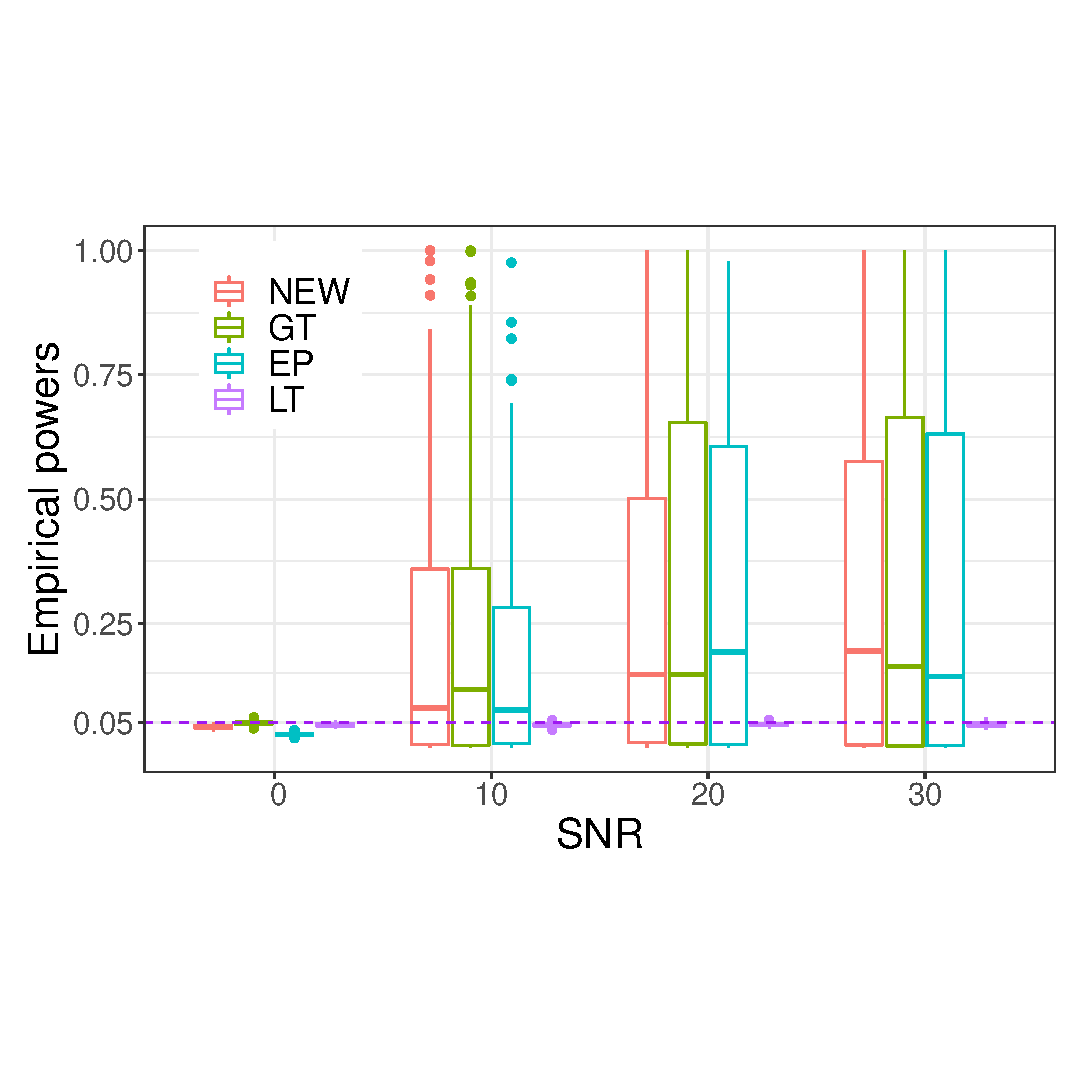
\includegraphics[width=0.45\textwidth]{code/figure/50_uniform_t_dense}
    }
    \subfigure[$n=50$, $\epsilon_1\sim t_9$. Sparse $\bbeta_b$.]{
        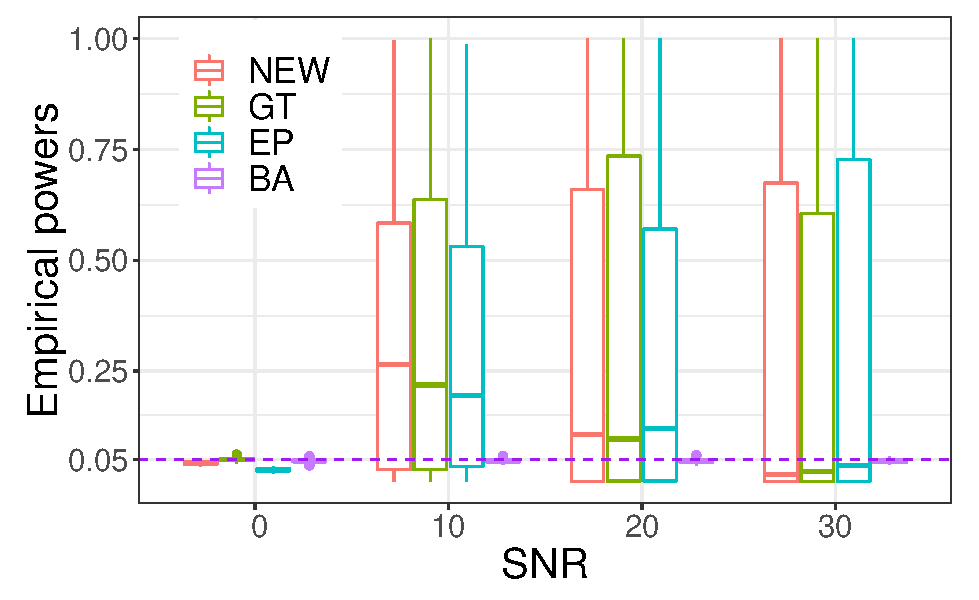
\includegraphics[width=0.45\textwidth]{code/figure/50_uniform_t_sparse}
    }
    \\
    \subfigure[$n=50$, $\epsilon_1\sim (\chi^2(4)-4)/\sqrt{8}$. Dense $\bbeta_b$.]{
        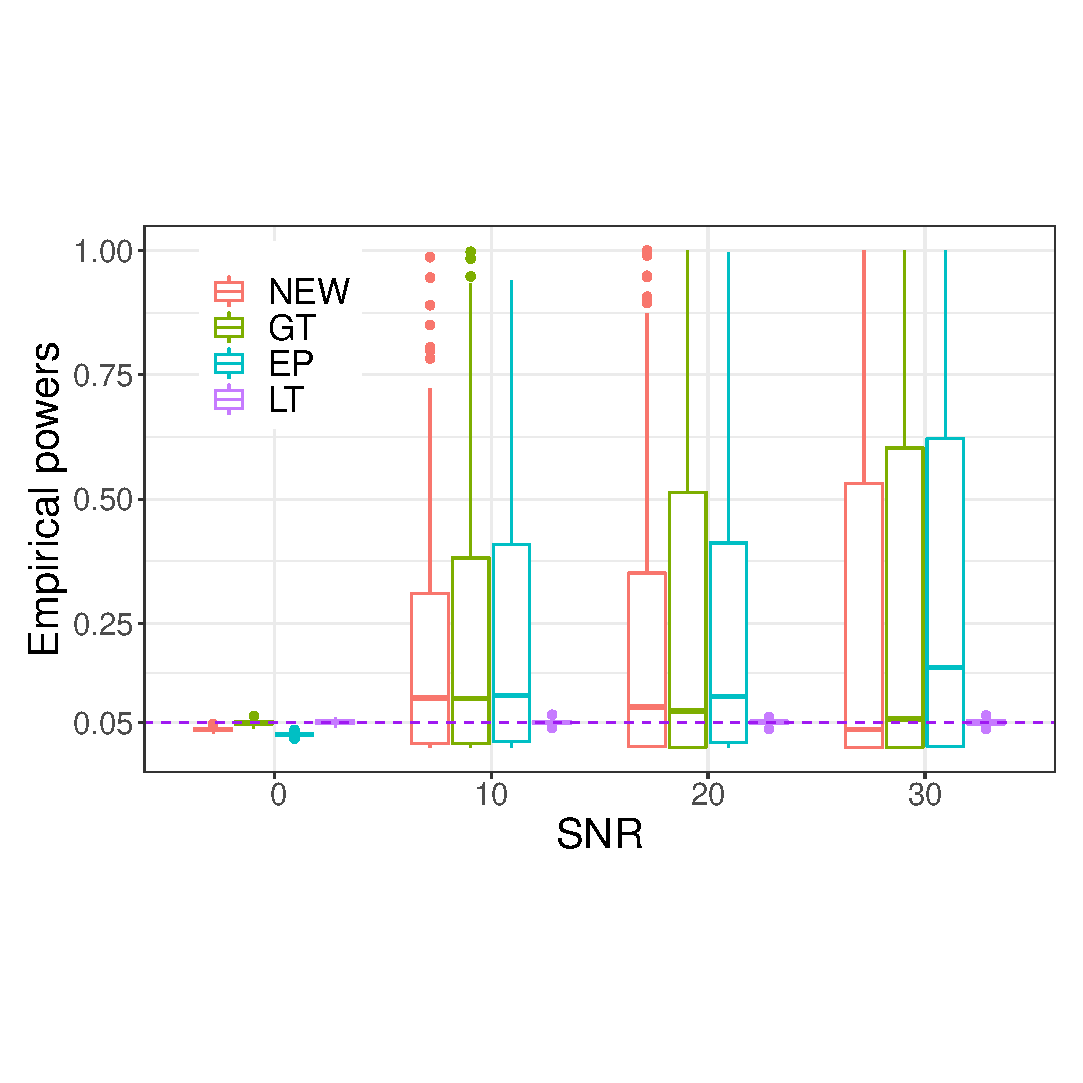
\includegraphics[width=0.45\textwidth]{code/figure/50_uniform_chi_dense}
    }
    \subfigure[$n=50$, $\epsilon_1\sim (\chi^2(4)-4)/\sqrt{8}$. Sparse $\bbeta_b$.]{
        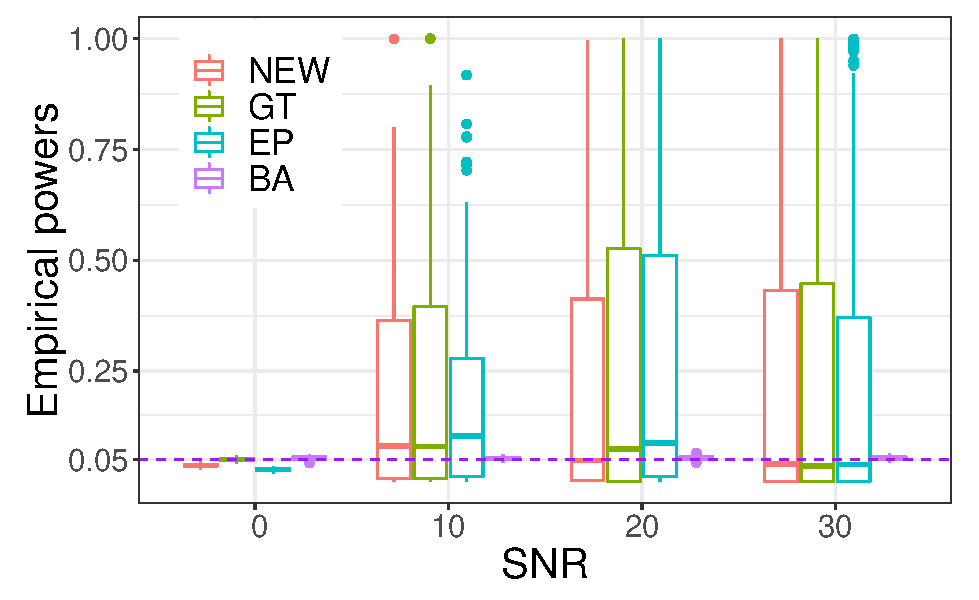
\includegraphics[width=0.45\textwidth]{code/figure/50_uniform_chi_sparse}
    }
    \\
    \subfigure[$n=100$, $\epsilon_1\sim t_9$. Dense $\bbeta_b$.]{
        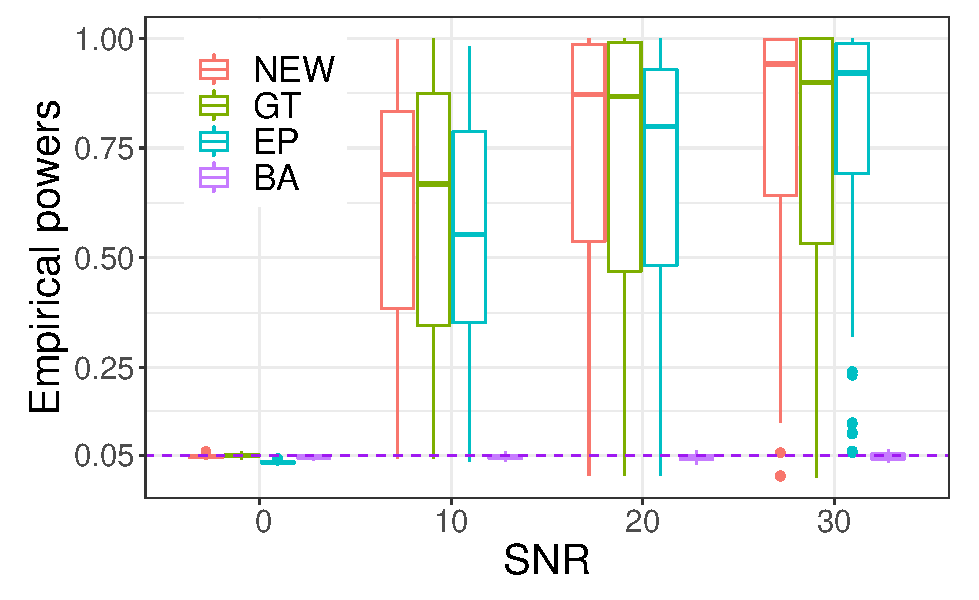
\includegraphics[width=0.45\textwidth]{code/figure/100_uniform_t_dense}
    }
    \subfigure[$n=100$, $\epsilon_1\sim t_9$. Sparse $\bbeta_b$.]{
        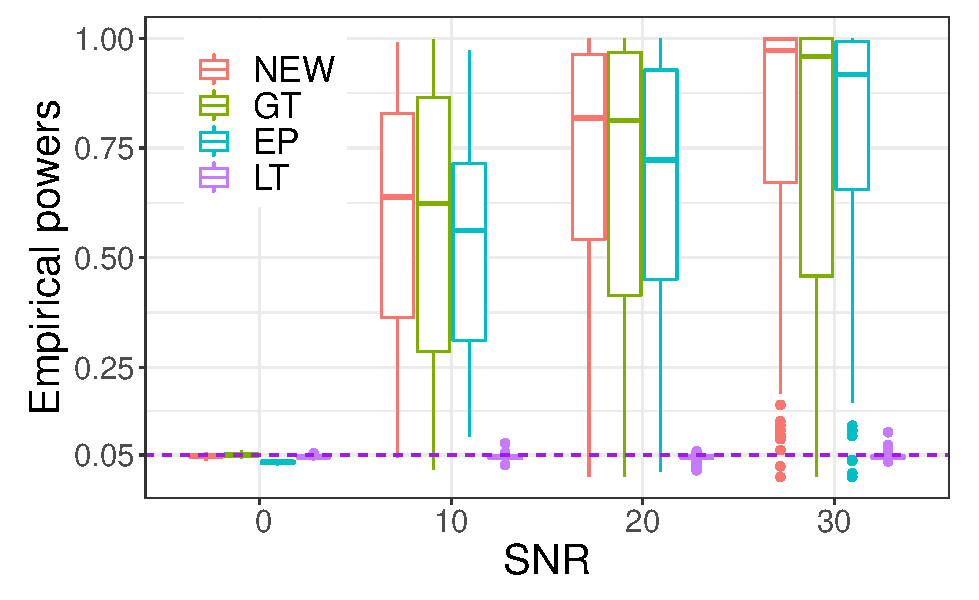
\includegraphics[width=0.45\textwidth]{code/figure/100_uniform_t_sparse}
    }
    \\
    \subfigure[$n=100$, $\epsilon_1\sim (\chi^2(4)-4)/\sqrt{8}$. Dense $\bbeta_b$.]{
        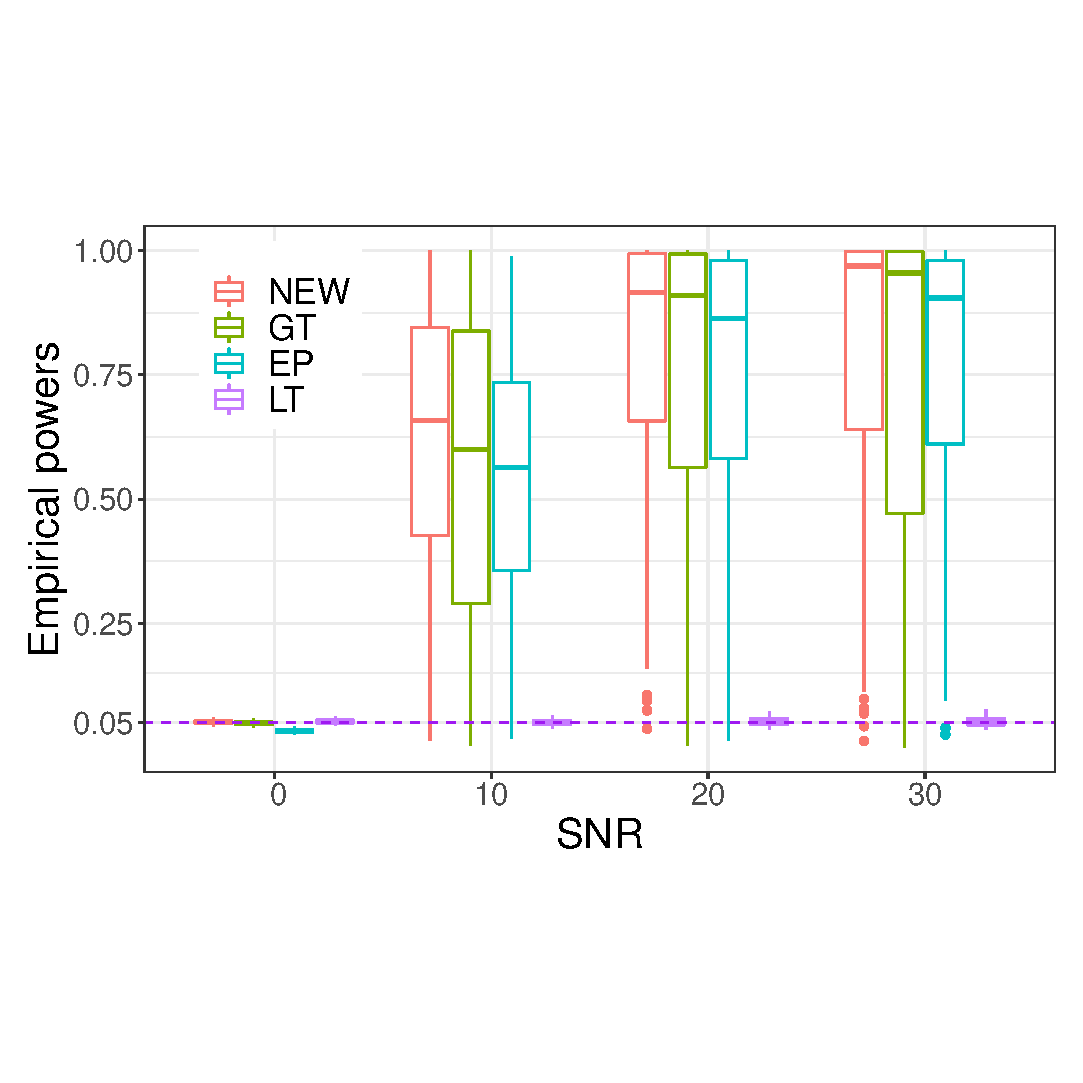
\includegraphics[width=0.45\textwidth]{code/figure/100_uniform_chi_dense}
    }
    \subfigure[$n=100$, $\epsilon_1\sim (\chi^2(4)-4)/\sqrt{8}$. Sparse $\bbeta_b$.]{
        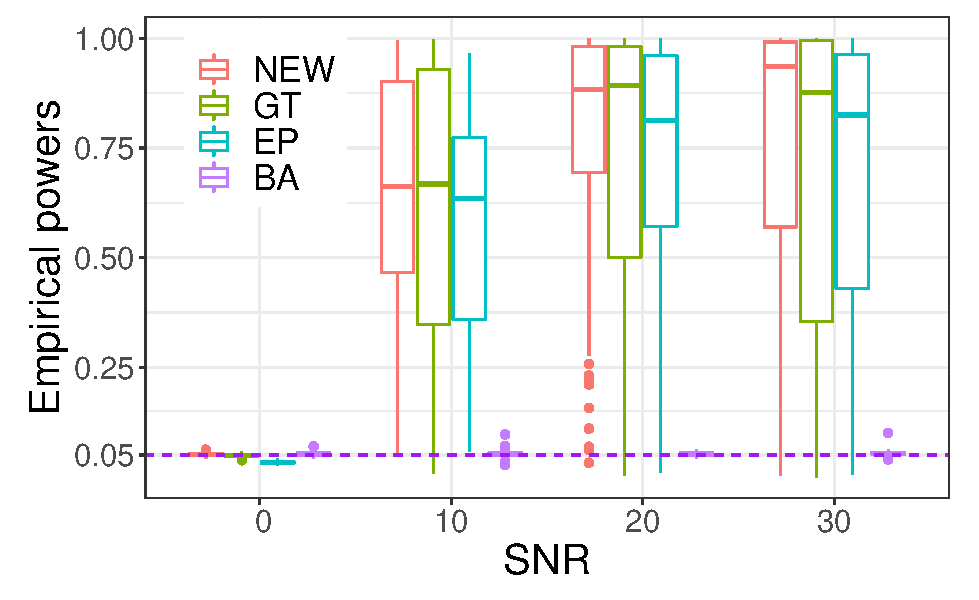
\includegraphics[width=0.45\textwidth]{code/figure/100_uniform_chi_sparse}
    }
    \caption{Box plots of the empirical powers based on $100$ independently generated $\bbeta_b$.
        $\BX_b$ is generated by Model I.
    }\label{fig:1}
\end{figure}

\begin{figure}
    \centering 
    \subfigure[$n=50$, $\epsilon_1\sim t_9$. Dense $\bbeta_b$.]{
        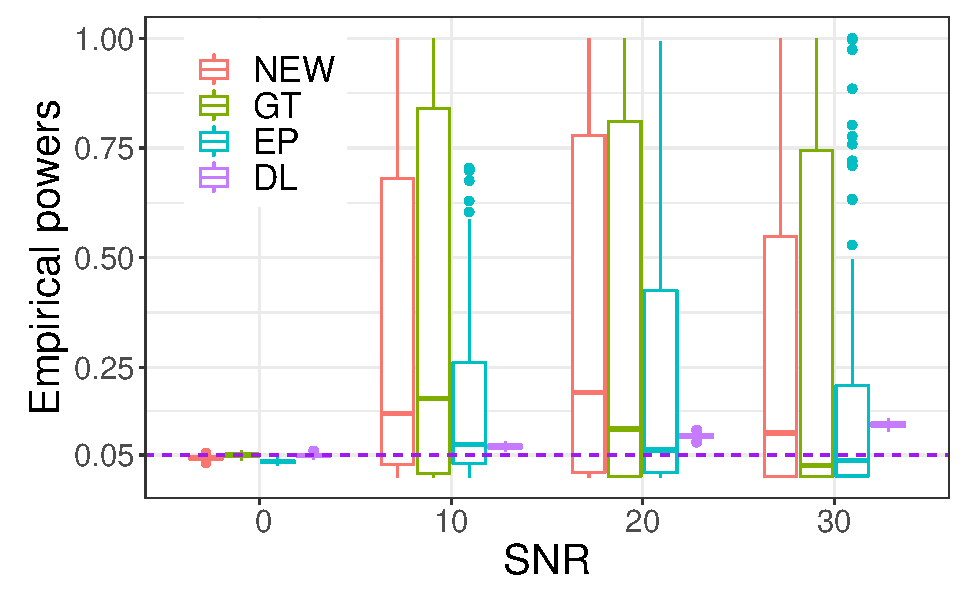
\includegraphics[width=0.45\textwidth]{code/figure/50_equalCor_t_dense}
    }
    \subfigure[$n=50$, $\epsilon_1\sim t_9$. Sparse $\bbeta_b$.]{
        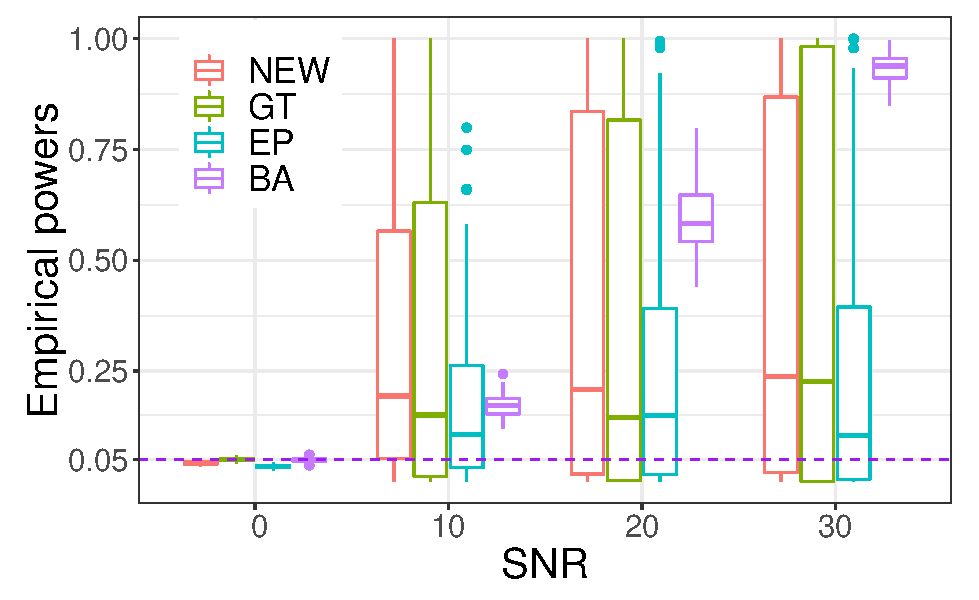
\includegraphics[width=0.45\textwidth]{code/figure/50_equalCor_t_sparse}
    }
    \\
    \subfigure[$n=50$, $\epsilon_1\sim (\chi^2(4)-4)/\sqrt{8}$. Dense $\bbeta_b$.]{
        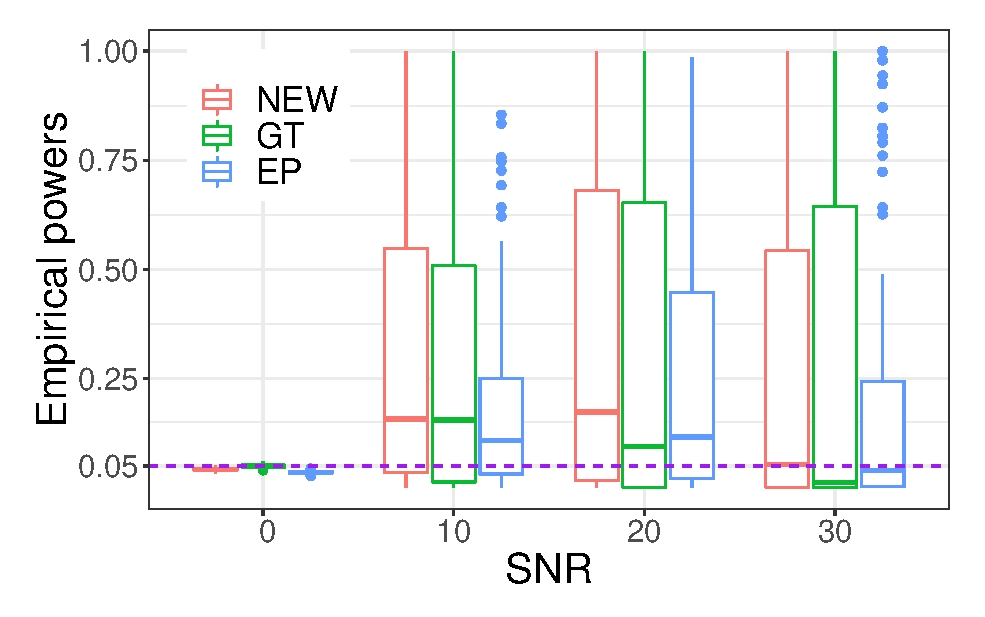
\includegraphics[width=0.45\textwidth]{code/figure/50_equalCor_chi_dense}
    }
    \subfigure[$n=50$, $\epsilon_1\sim (\chi^2(4)-4)/\sqrt{8}$. Sparse $\bbeta_b$.]{
        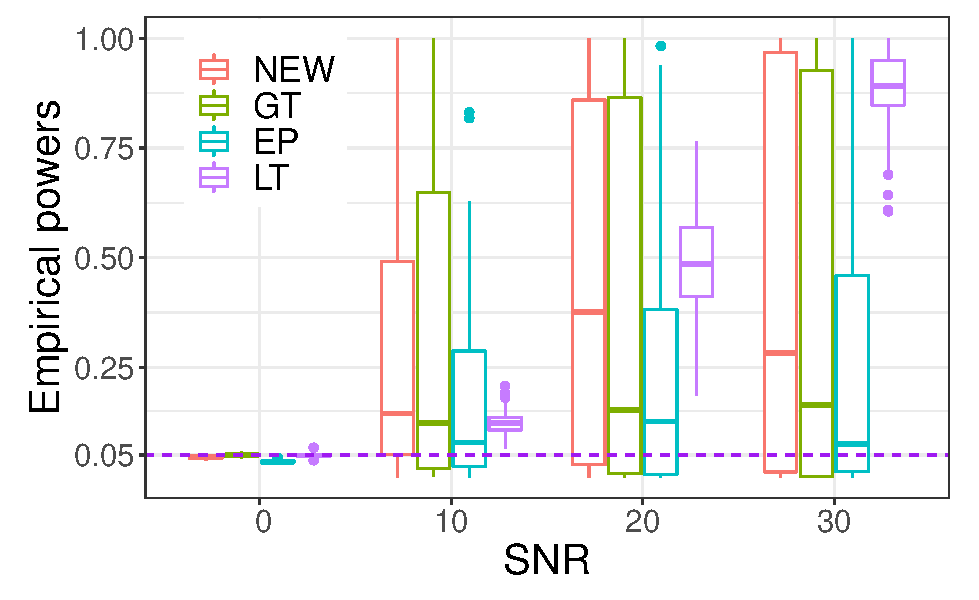
\includegraphics[width=0.45\textwidth]{code/figure/50_equalCor_chi_sparse}
    }
    \\
    \subfigure[$n=100$, $\epsilon_1\sim t_9$. Dense $\bbeta_b$.]{
        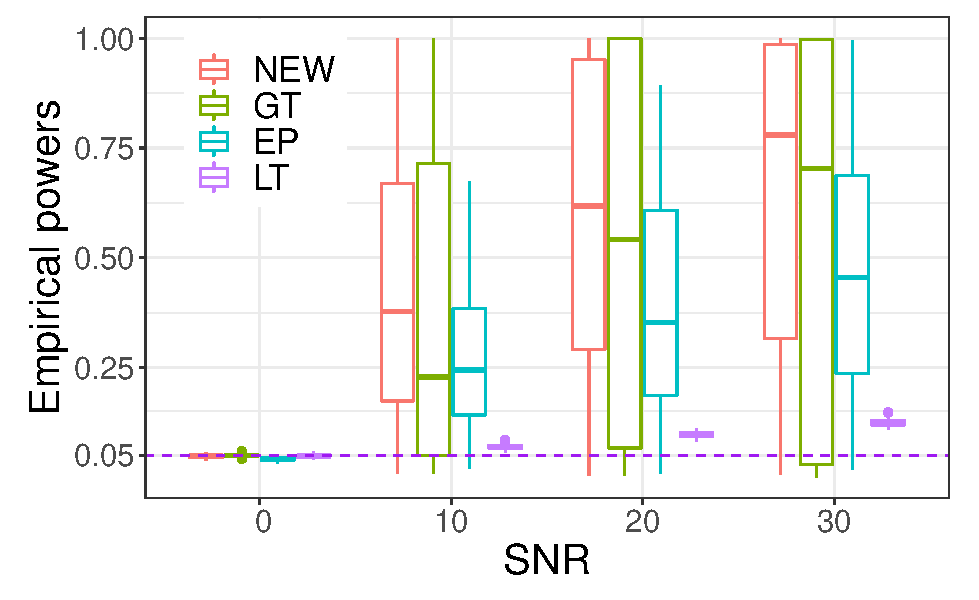
\includegraphics[width=0.45\textwidth]{code/figure/100_equalCor_t_dense}
    }
    \subfigure[$n=100$, $\epsilon_1\sim t_9$. Sparse $\bbeta_b$.]{
        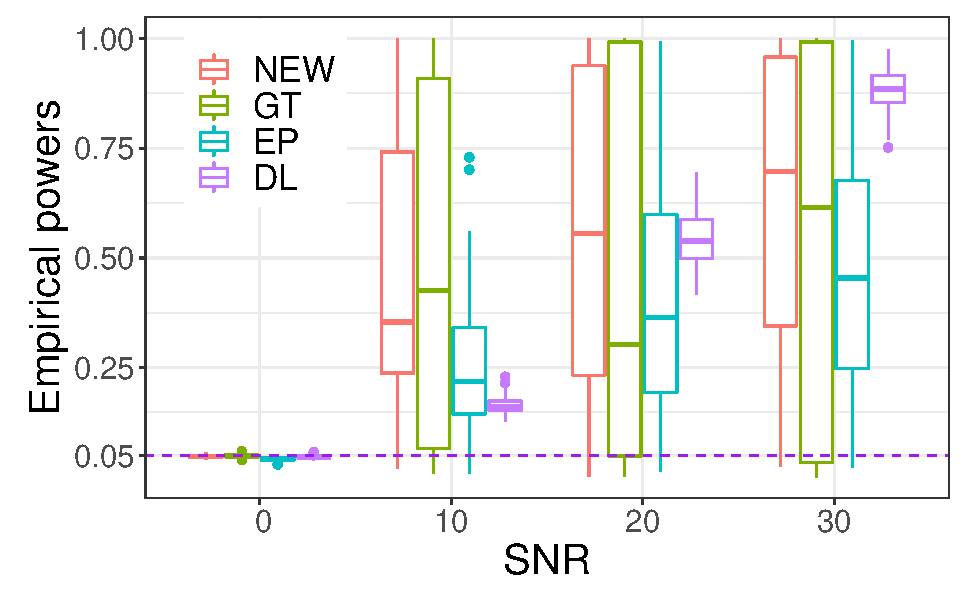
\includegraphics[width=0.45\textwidth]{code/figure/100_equalCor_t_sparse}
    }
    \\
    \subfigure[$n=100$, $\epsilon_1\sim (\chi^2(4)-4)/\sqrt{8}$. Dense $\bbeta_b$.]{
        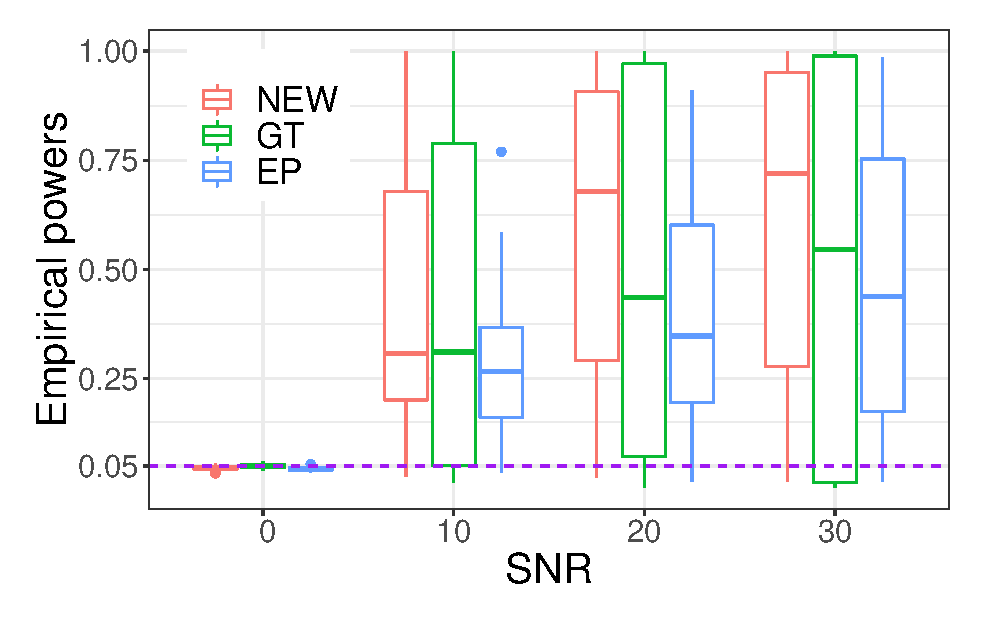
\includegraphics[width=0.45\textwidth]{code/figure/100_equalCor_chi_dense}
    }
    \subfigure[$n=100$, $\epsilon_1\sim (\chi^2(4)-4)/\sqrt{8}$. Sparse $\bbeta_b$.]{
        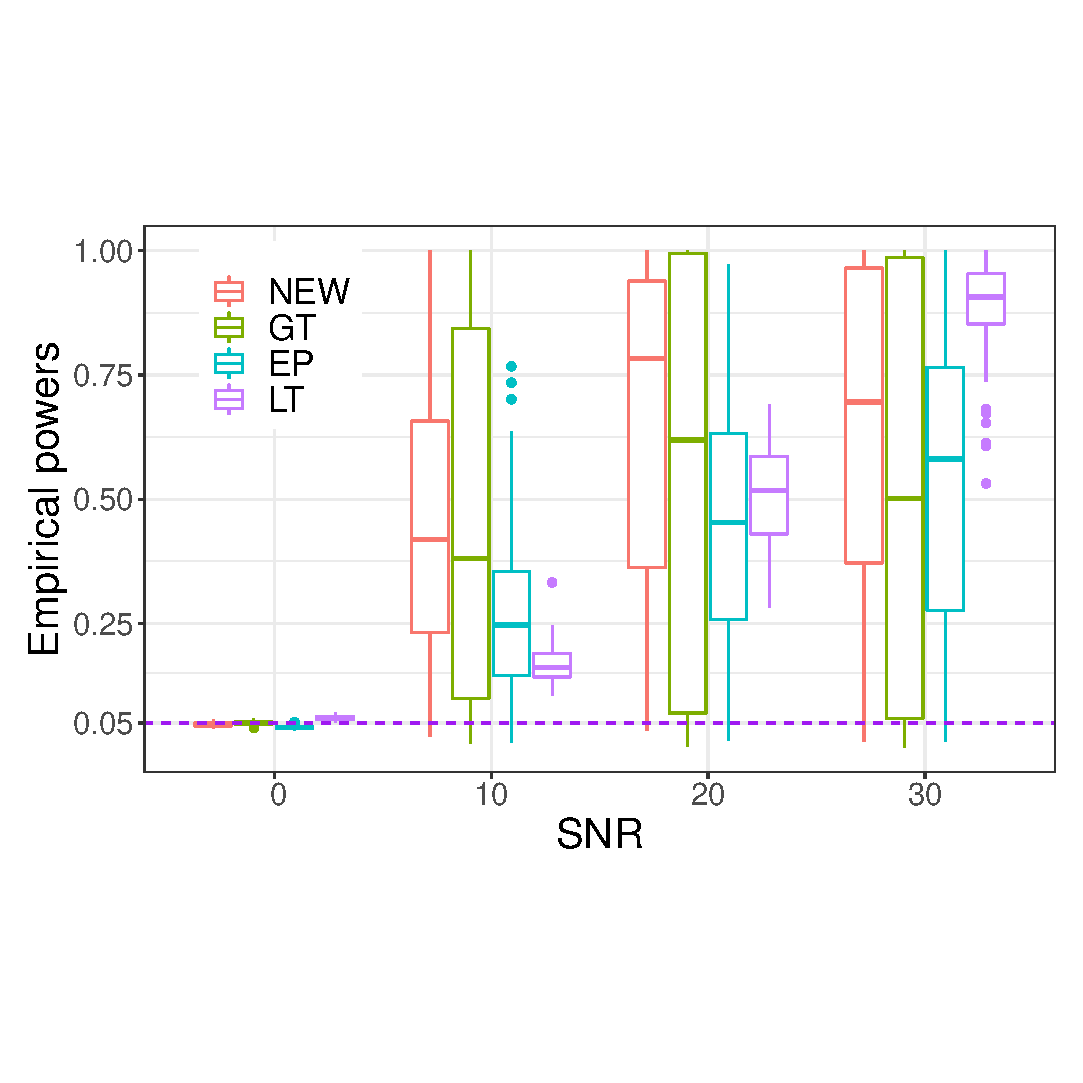
\includegraphics[width=0.45\textwidth]{code/figure/100_equalCor_chi_sparse}
    }
    \caption{Box plots of the empirical powers based on $100$ independently generated $\bbeta_b$.
$\BX_b$ is generated by Model II.
    }\label{fig:2}
\end{figure}

\begin{figure}
    \centering 
    \subfigure[$n=50$, $\epsilon_1\sim t_9$. Dense $\bbeta_b$.]{
        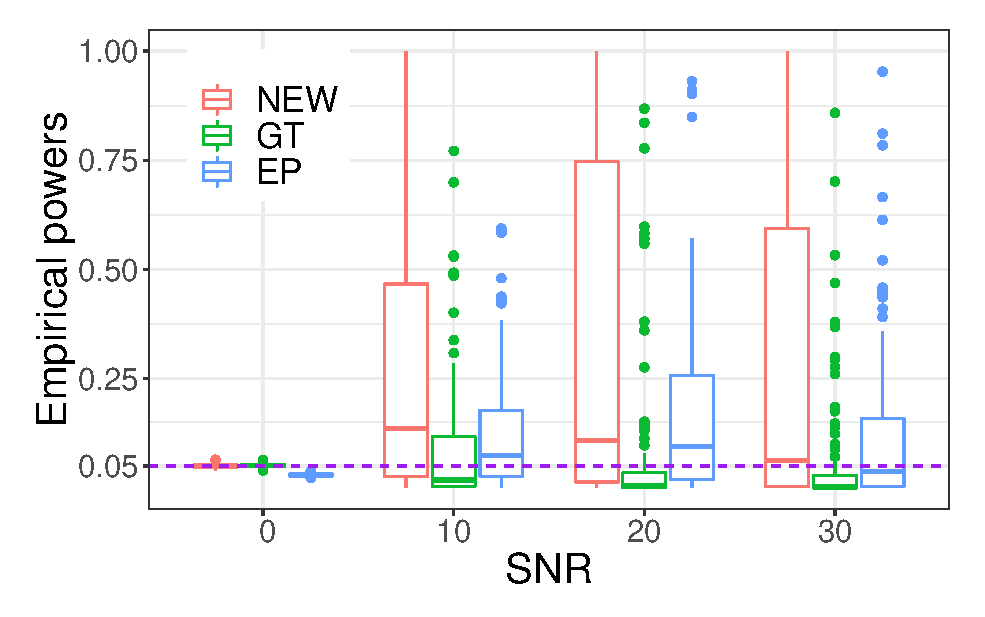
\includegraphics[width=0.45\textwidth]{code/figure/50_factor_t_dense}
    }
    \subfigure[$n=50$, $\epsilon_1\sim t_9$. Sparse $\bbeta_b$.]{
        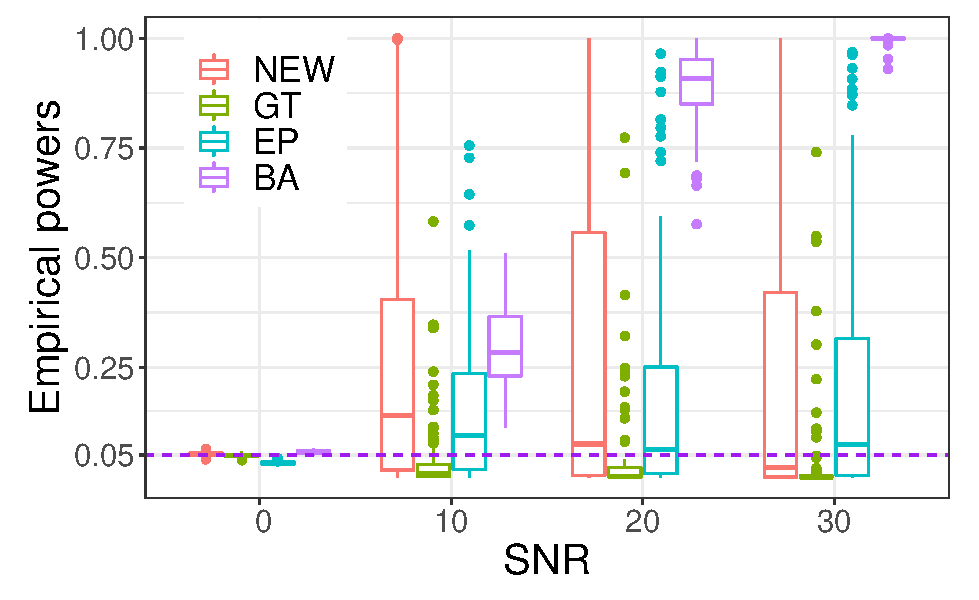
\includegraphics[width=0.45\textwidth]{code/figure/50_factor_t_sparse}
    }
    \\
    \subfigure[$n=50$, $\epsilon_1\sim (\chi^2(4)-4)/\sqrt{8}$. Dense $\bbeta_b$.]{
        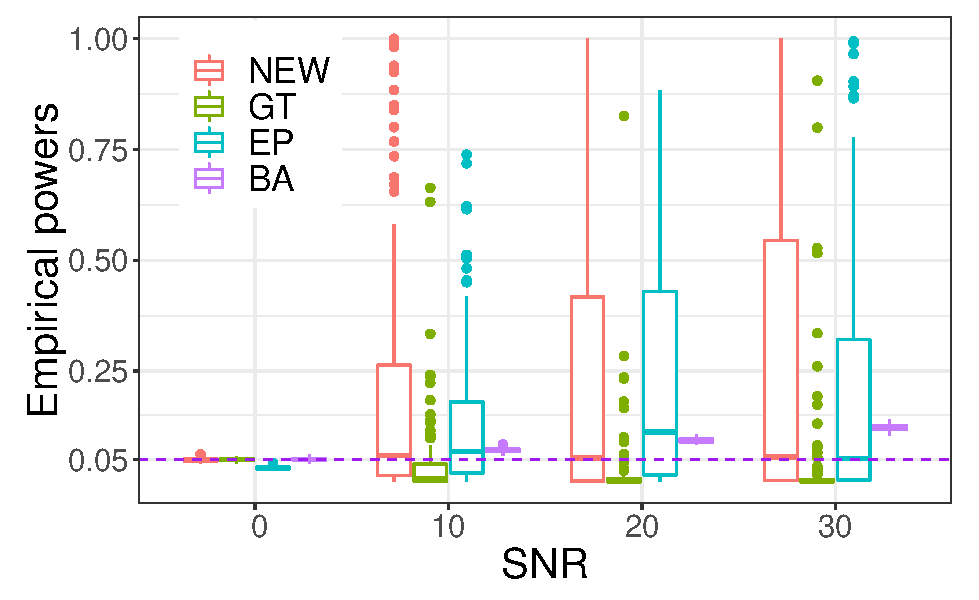
\includegraphics[width=0.45\textwidth]{code/figure/50_factor_chi_dense}
    }
    \subfigure[$n=50$, $\epsilon_1\sim (\chi^2(4)-4)/\sqrt{8}$. Sparse $\bbeta_b$.]{
        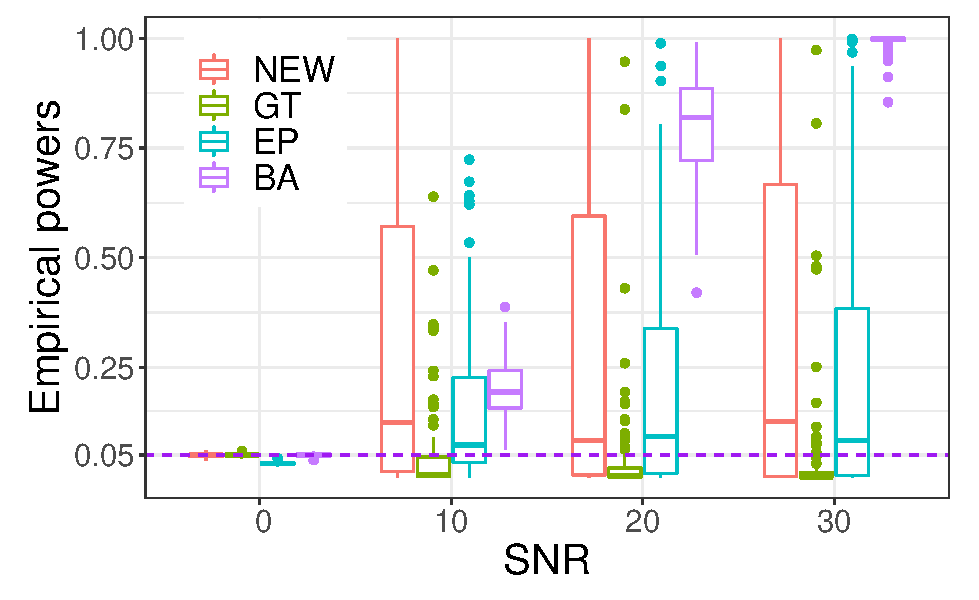
\includegraphics[width=0.45\textwidth]{code/figure/50_factor_chi_sparse}
    }
    \\
    \subfigure[$n=100$, $\epsilon_1\sim t_9$. Dense $\bbeta_b$.]{
        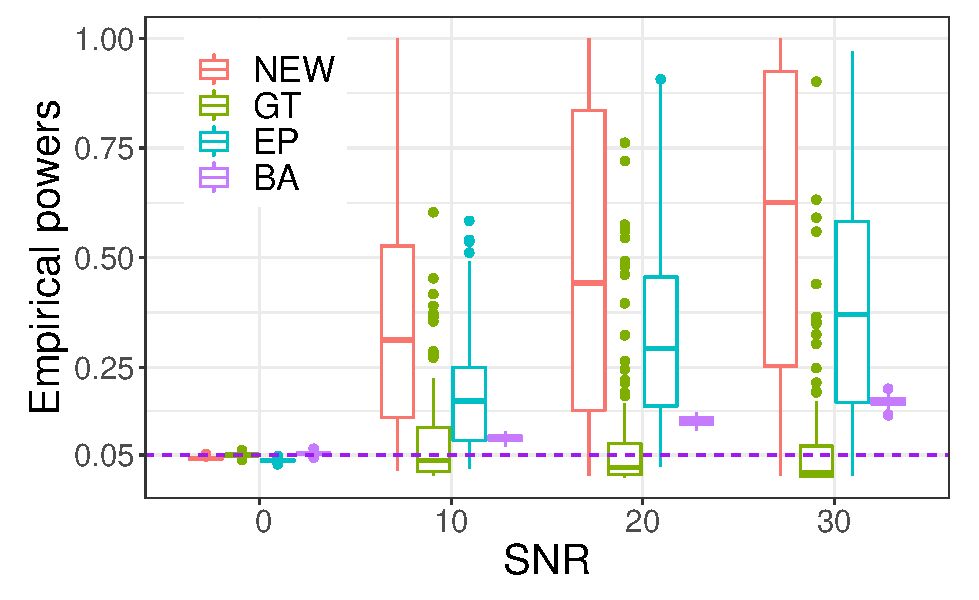
\includegraphics[width=0.45\textwidth]{code/figure/100_factor_t_dense}
    }
    \subfigure[$n=100$, $\epsilon_1\sim t_9$. Sparse $\bbeta_b$.]{
        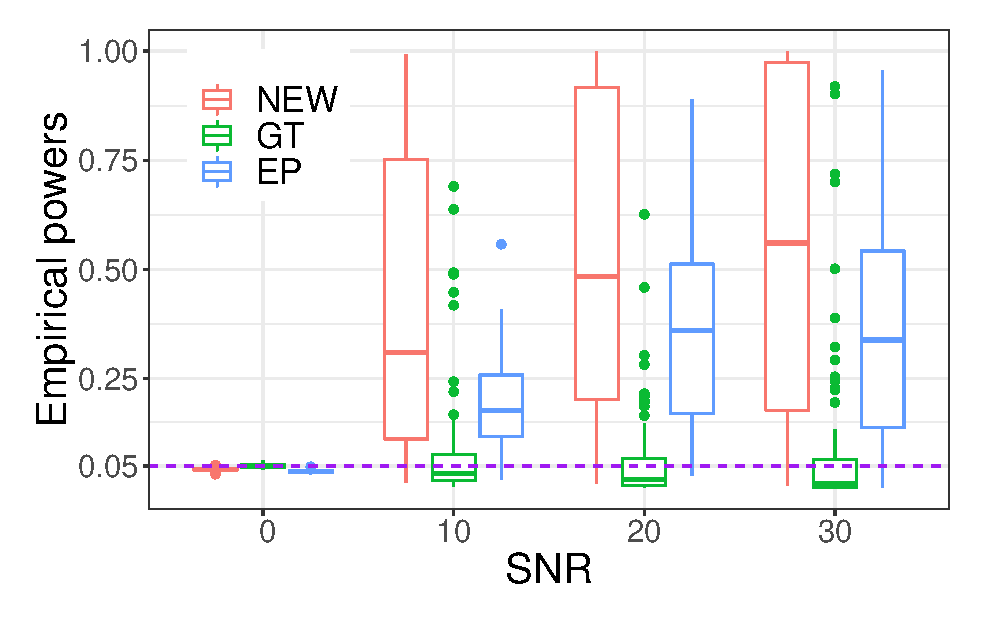
\includegraphics[width=0.45\textwidth]{code/figure/100_factor_t_sparse}
    }
    \\
    \subfigure[$n=100$, $\epsilon_1\sim (\chi^2(4)-4)/\sqrt{8}$. Dense $\bbeta_b$.]{
        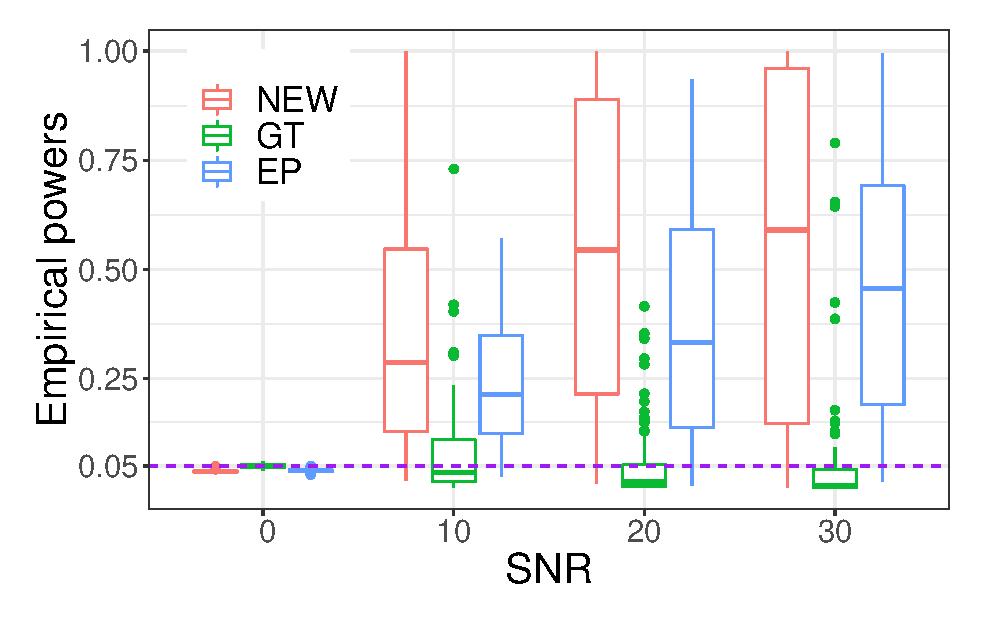
\includegraphics[width=0.45\textwidth]{code/figure/100_factor_chi_dense}
    }
    \subfigure[$n=100$, $\epsilon_1\sim (\chi^2(4)-4)/\sqrt{8}$. Sparse $\bbeta_b$.]{
        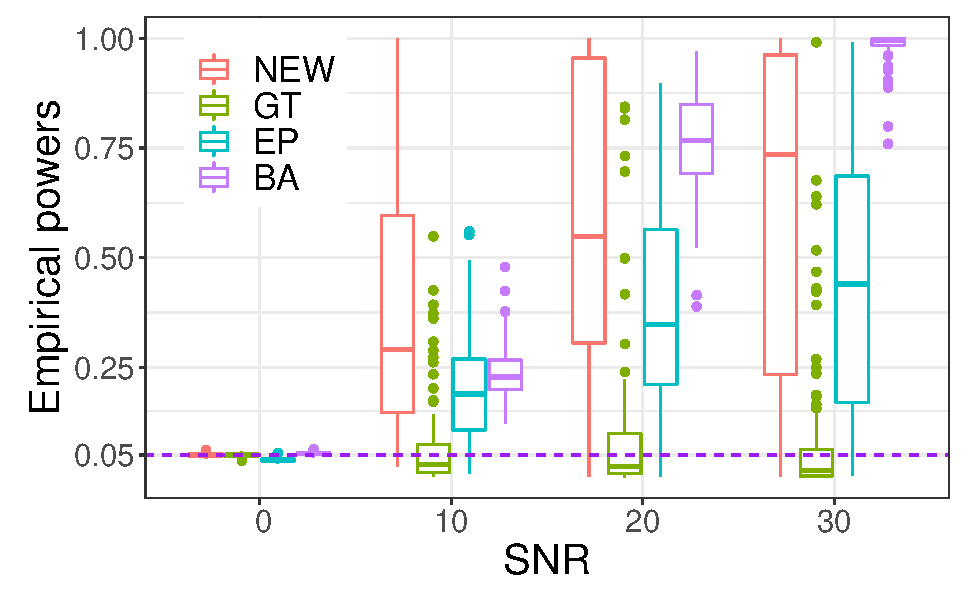
\includegraphics[width=0.45\textwidth]{code/figure/100_factor_chi_sparse}
    }
    \caption{Box plots of the empirical powers based on $100$ independently generated $\bbeta_b$.
$\BX_b$ is generated by Model III.
    }\label{fig:3}
\end{figure}
\begin{figure}
    \centering 
    \subfigure[$n=50$, $\epsilon_1\sim t_9$. Dense $\bbeta_b$.]{
        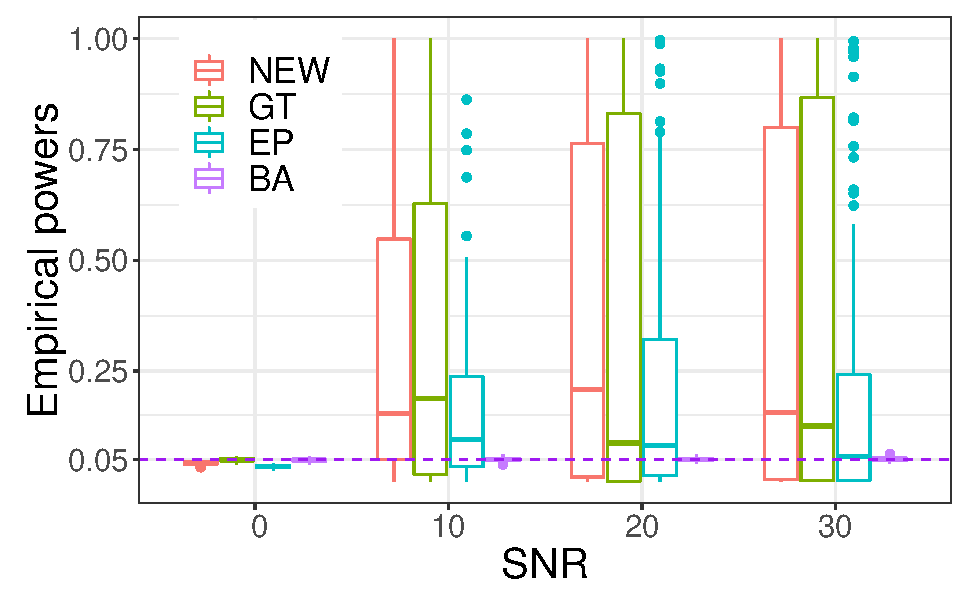
\includegraphics[width=0.45\textwidth]{code/figure/50_rowCor_t_dense}
    }
    \subfigure[$n=50$, $\epsilon_1\sim t_9$. Sparse $\bbeta_b$.]{
        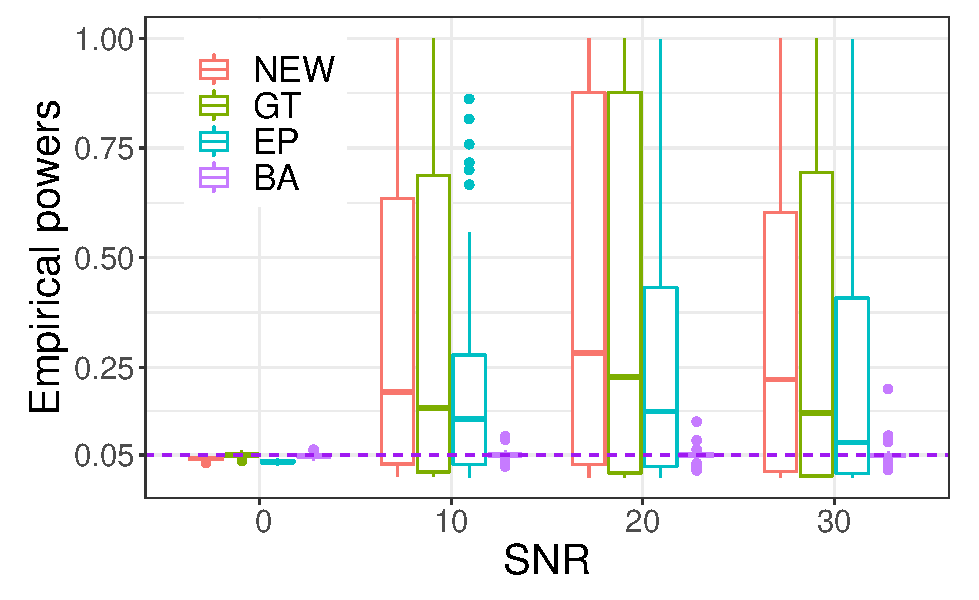
\includegraphics[width=0.45\textwidth]{code/figure/50_rowCor_t_sparse}
    }
    \\
    \subfigure[$n=50$, $\epsilon_1\sim (\chi^2(4)-4)/\sqrt{8}$. Dense $\bbeta_b$.]{
        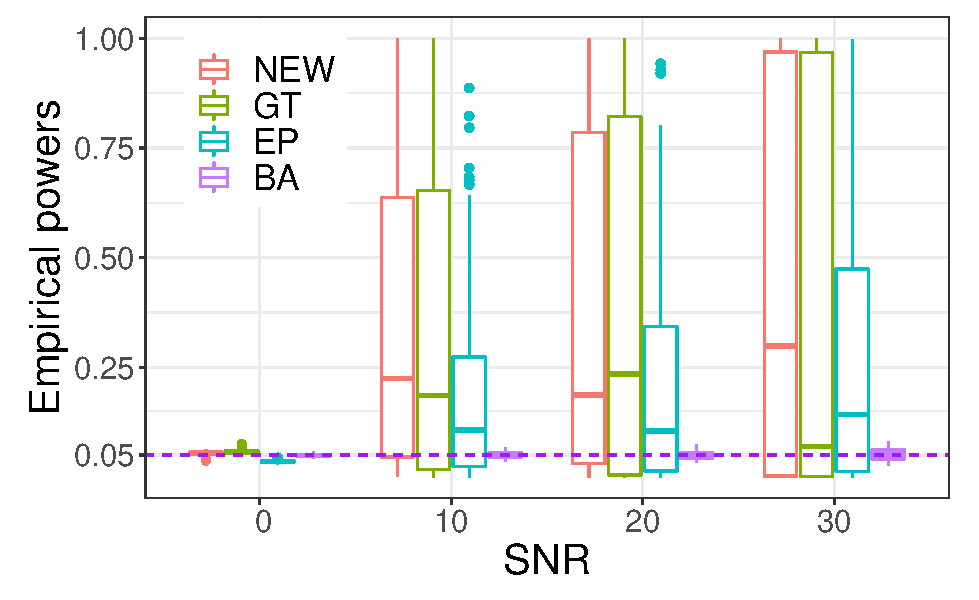
\includegraphics[width=0.45\textwidth]{code/figure/50_rowCor_chi_dense}
    }
    \subfigure[$n=50$, $\epsilon_1\sim (\chi^2(4)-4)/\sqrt{8}$. Sparse $\bbeta_b$.]{
        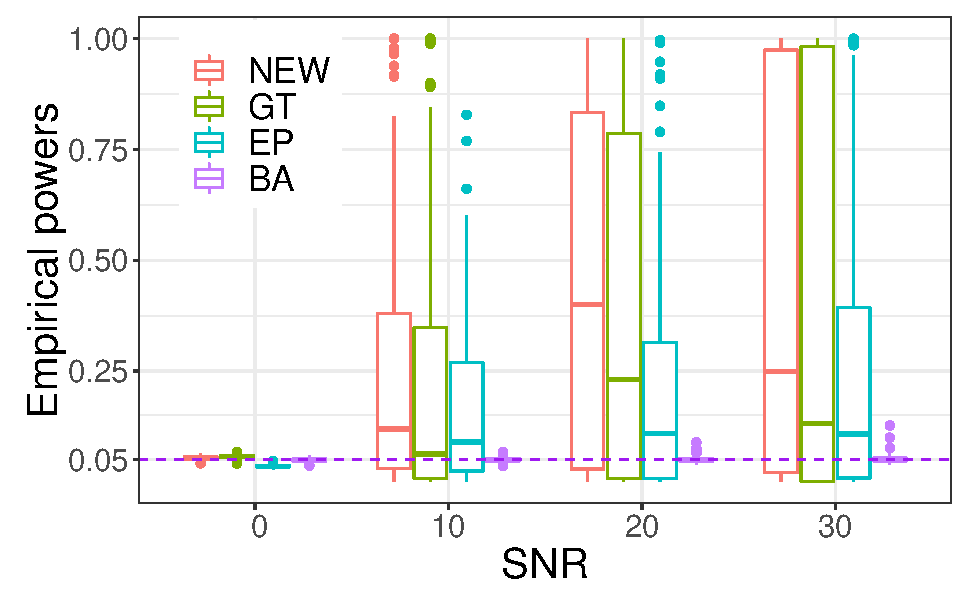
\includegraphics[width=0.45\textwidth]{code/figure/50_rowCor_chi_sparse}
    }
    \\
    \subfigure[$n=100$, $\epsilon_1\sim t_9$. Dense $\bbeta_b$.]{
        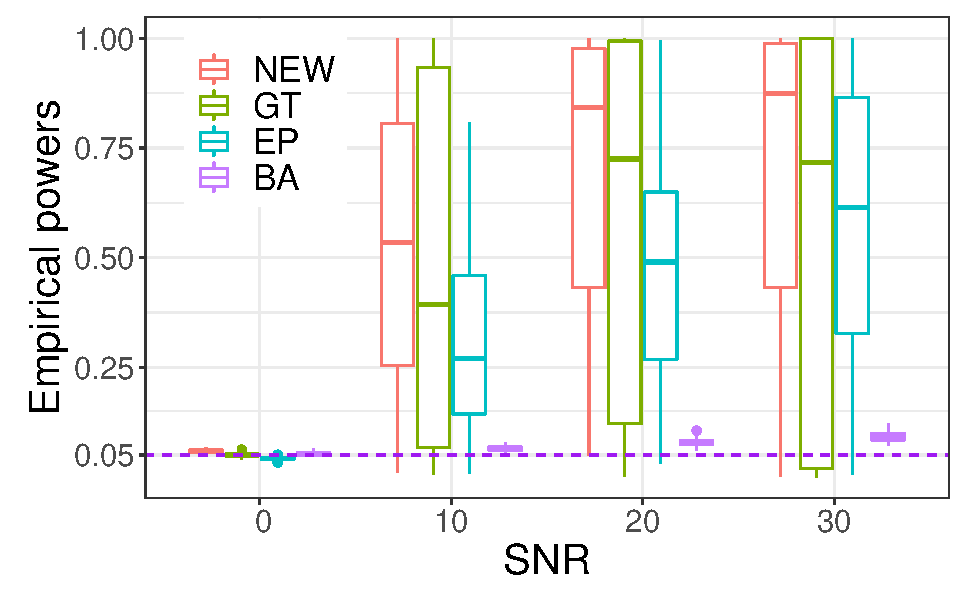
\includegraphics[width=0.45\textwidth]{code/figure/100_rowCor_t_dense}
    }
    \subfigure[$n=100$, $\epsilon_1\sim t_9$. Sparse $\bbeta_b$.]{
        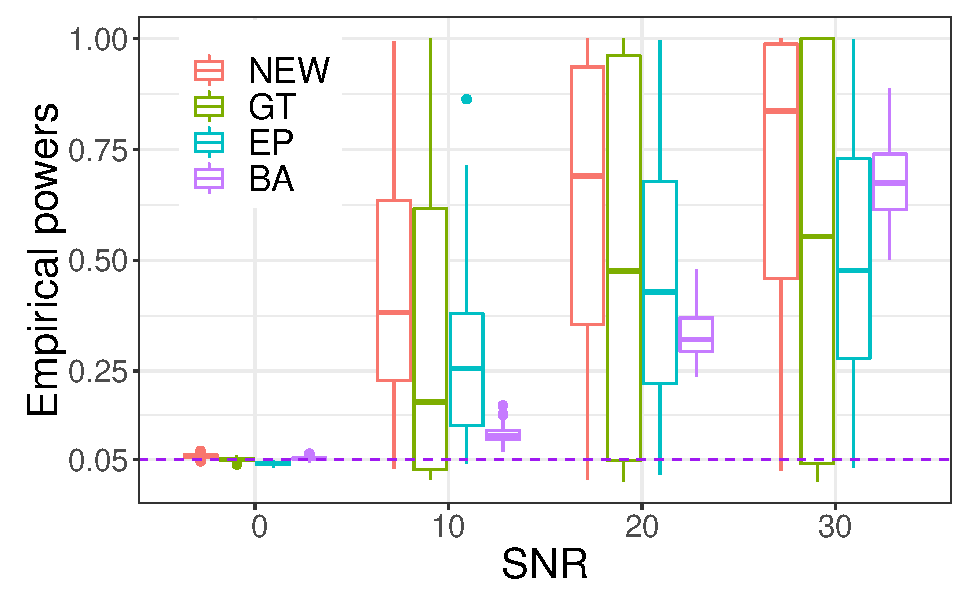
\includegraphics[width=0.45\textwidth]{code/figure/100_rowCor_t_sparse}
    }
    \\
    \subfigure[$n=100$, $\epsilon_1\sim (\chi^2(4)-4)/\sqrt{8}$. Dense $\bbeta_b$.]{
        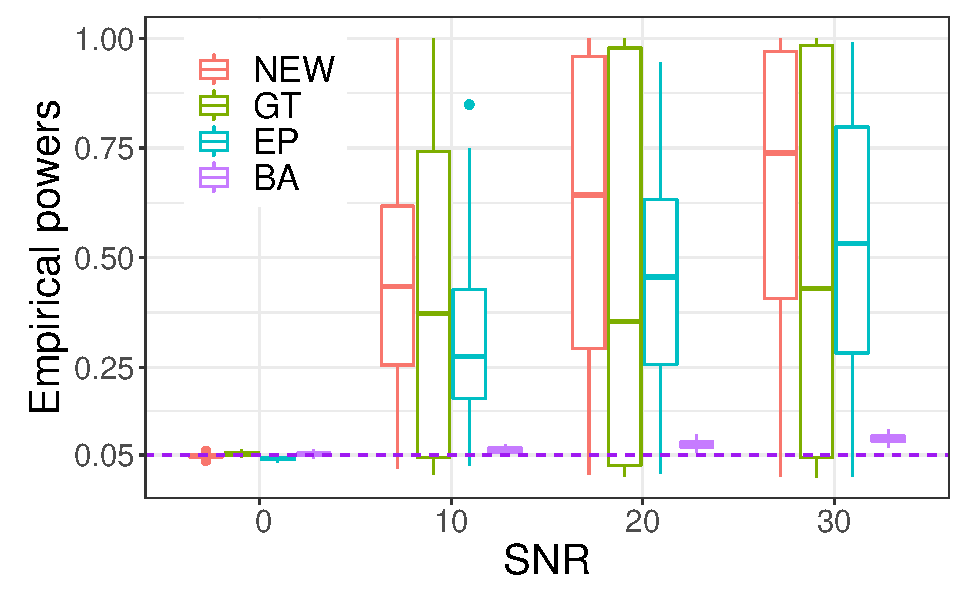
\includegraphics[width=0.45\textwidth]{code/figure/100_rowCor_chi_dense}
    }
    \subfigure[$n=100$, $\epsilon_1\sim (\chi^2(4)-4)/\sqrt{8}$. Sparse $\bbeta_b$.]{
        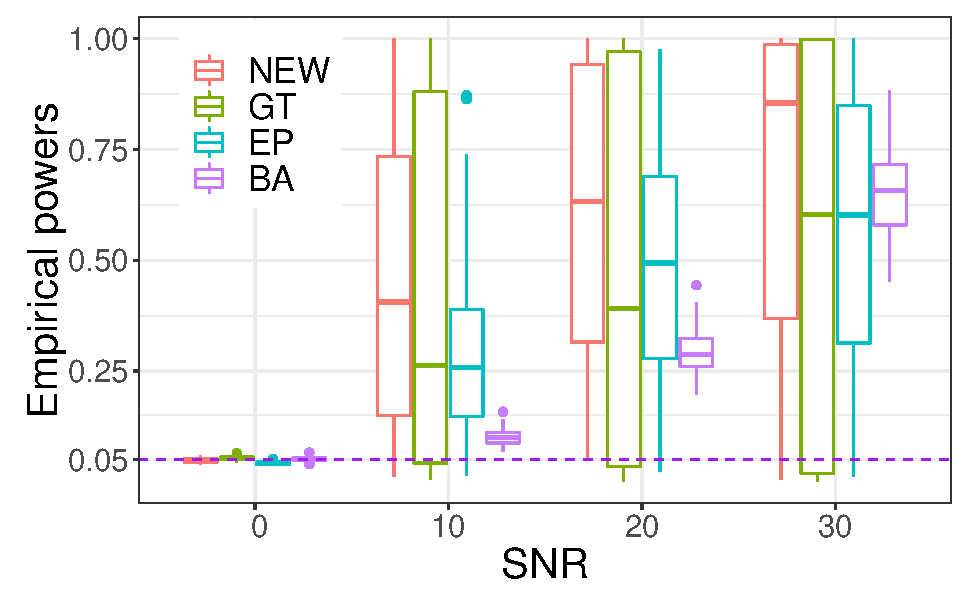
\includegraphics[width=0.45\textwidth]{code/figure/100_rowCor_chi_sparse}
    }
    \caption{Box plots of the empirical powers based on $100$ independently generated $\bbeta_b$.
$\BX_b$ is generated by Model IV.
    }\label{fig:4}
\end{figure}


%
%\begin{table*}[ht]
%    \caption{
%        Empirical size and power under Toeplitz structure; $q=10$, $p=1000$, $\alpha=0.05$.
%    }
%\label{table1}
%    \centering
%    \begin{tabular}{clcccccccc}
%          \toprule
%          & & \multicolumn{4}{c}{$\epsilon_1\sim t_8$} &\multicolumn{4}{c}{$\epsilon_1\sim (\chi^2(4)-4)/\sqrt{8}$}\\
%          \cmidrule(r){3-6}\cmidrule(r){7-10}
%          & & \multicolumn{2}{c}{Dense $\bbeta_b$} & \multicolumn{2}{c}{Sparse $\bbeta_b$} & \multicolumn{2}{c}{Dense $\bbeta_b$}& \multicolumn{2}{c}{Sparse $\bbeta_b$}\\
%          \cmidrule(r){3-4}  \cmidrule(r){5-6} \cmidrule(r){7-8}  \cmidrule(r){9-10}
%           $n$&SNR & NEW & GT & NEW & GT & NEW & GT & NEW & GT \\ 
%            \midrule
%        $50$ &0 (size)
% & 0.0590 & 0.0546 & 0.0348 & 0.0542 & 0.0346 & 0.0486 & 0.0334 & 0.0498 \\ 
%  &5 & 0.3650 & 0.3438 & 0.2818 & 0.3500 & 0.3474 & 0.3954 & 0.3304 & 0.3786 \\ 
%  &10 & 0.5266 & 0.4850 & 0.4584 & 0.4896 & 0.5036 & 0.5314 & 0.5034 & 0.5396 \\ 
%  &15 & 0.6282 & 0.5654 & 0.5638 & 0.5822 & 0.5812 & 0.5892 & 0.5800 & 0.5884 \\ 
%  &20 & 0.6980 & 0.6114 & 0.6222 & 0.6298 & 0.6390 & 0.6370 & 0.6204 & 0.6192 \\ 
%  &25 & 0.7228 & 0.6412 & 0.6466 & 0.6398 & 0.6610 & 0.6504 & 0.6550 & 0.6374 \\ 
%  &30 & 0.7362 & 0.6418 & 0.6920 & 0.6878 & 0.6932 & 0.6700 & 0.6706 & 0.6518 \\ 
%        \midrule
%$100$&0 (size) 
%& 0.0620 & 0.0510 & 0.0380 & 0.0504 & 0.0530 & 0.0478 & 0.0482 & 0.0514 \\ 
%  &5 & 0.4572 & 0.5056 & 0.3630 & 0.4962 & 0.5534 & 0.6048 & 0.4908 & 0.5988 \\ 
%  &10 & 0.7496 & 0.7664 & 0.6562 & 0.7478 & 0.8404 & 0.8468 & 0.7950 & 0.8198 \\ 
%  &15 & 0.8830 & 0.8658 & 0.8330 & 0.8666 & 0.9296 & 0.9134 & 0.9110 & 0.9066 \\ 
%  &20 & 0.9500 & 0.9176 & 0.9100 & 0.9224 & 0.9660 & 0.9504 & 0.9586 & 0.9506 \\ 
%  &25 & 0.9682 & 0.9460 & 0.9532 & 0.9470 & 0.9832 & 0.9682 & 0.9782 & 0.9656 \\ 
%  &30 & 0.9836 & 0.9604 & 0.9676 & 0.9664 & 0.9924 & 0.9770 & 0.9874 & 0.9730 \\ 
%        \bottomrule
%    \end{tabular}
%\end{table*}
%
%\begin{table*}[ht]
%    \caption{
%        Empirical size and power under equal correlation structure; $q=10$, $p=1000$, $\alpha=0.05$.
%    }
%\label{table2}
%    \centering
%    \begin{tabular}{clcccccccc}
%          \toprule
%          & & \multicolumn{4}{c}{$\epsilon_1\sim t_8$} &\multicolumn{4}{c}{$\epsilon_1\sim (\chi^2(4)-4)/\sqrt{8}$}\\
%          \cmidrule(r){3-6}\cmidrule(r){7-10}
%          & & \multicolumn{2}{c}{Dense $\bbeta_b$} & \multicolumn{2}{c}{Sparse $\bbeta_b$} & \multicolumn{2}{c}{Dense $\bbeta_b$}& \multicolumn{2}{c}{Sparse $\bbeta_b$}\\
%          \cmidrule(r){3-4}  \cmidrule(r){5-6} \cmidrule(r){7-8}  \cmidrule(r){9-10}
%           $n$&SNR & NEW & GT & NEW & GT & NEW & GT & NEW & GT \\ 
%            \midrule
%        $50$ &0 (size)
%& 0.0458 & 0.0492 & 0.0464 & 0.0502 & 0.0524 & 0.0530 & 0.0520 & 0.0516 \\ 
%  &5 & 0.2524 & 0.2594 & 0.2640 & 0.2674 & 0.2634 & 0.2630 & 0.2914 & 0.2836 \\ 
%  &10 & 0.3228 & 0.3102 & 0.3396 & 0.3278 & 0.3316 & 0.3070 & 0.3758 & 0.3432 \\ 
%  &15 & 0.3530 & 0.3382 & 0.3732 & 0.3520 & 0.3598 & 0.3332 & 0.3960 & 0.3654 \\ 
%  &20 & 0.3754 & 0.3498 & 0.3862 & 0.3644 & 0.3628 & 0.3320 & 0.4146 & 0.3728 \\ 
%  &25 & 0.3872 & 0.3566 & 0.4022 & 0.3694 & 0.3810 & 0.3394 & 0.4228 & 0.3822 \\ 
%  &30 & 0.4130 & 0.3736 & 0.4006 & 0.3684 & 0.3830 & 0.3478 & 0.4352 & 0.3930 \\ 
%        \midrule
%$100$&0 (size) 
% & 0.0458 & 0.0540 & 0.0482 & 0.0462 & 0.0406 & 0.0526 & 0.0464 & 0.0480 \\ 
%  &5 & 0.2472 & 0.3176 & 0.2570 & 0.3158 & 0.2914 & 0.3584 & 0.3142 & 0.3496 \\ 
%  &10 & 0.3818 & 0.4078 & 0.3950 & 0.4108 & 0.4298 & 0.4482 & 0.4582 & 0.4402 \\ 
%  &15 & 0.4820 & 0.4720 & 0.4788 & 0.4594 & 0.5172 & 0.5008 & 0.5542 & 0.4820 \\ 
%  &20 & 0.5292 & 0.4900 & 0.5414 & 0.4928 & 0.5742 & 0.5212 & 0.5988 & 0.5090 \\ 
%  &25 & 0.5700 & 0.5040 & 0.5984 & 0.5200 & 0.6018 & 0.5338 & 0.6262 & 0.5164 \\ 
%  &30 & 0.5972 & 0.5202 & 0.6172 & 0.5296 & 0.6392 & 0.5508 & 0.6582 & 0.5336 \\ 
%        \bottomrule
%    \end{tabular}
%\end{table*}
%
%\begin{table*}[ht]
%    \caption{
%        Empirical size and power under the design matrix of Bacillus subtilis gene expression data; $n=71$, $q=10$, $p=4078$, $\alpha=0.05$.
%    }
%\label{table3}
%    \centering
%    \begin{tabular}{lcccccccc}
%          \toprule
%           & \multicolumn{4}{c}{$\epsilon_1\sim t_8$} &\multicolumn{4}{c}{$\epsilon_1\sim (\chi^2(4)-4)/\sqrt{8}$}\\
%          \cmidrule(r){2-5}\cmidrule(r){6-9}
%           & \multicolumn{2}{c}{Dense $\bbeta_b$} & \multicolumn{2}{c}{Sparse $\bbeta_b$} & \multicolumn{2}{c}{Dense $\bbeta_b$}& \multicolumn{2}{c}{Sparse $\bbeta_b$}\\
%          \cmidrule(r){2-3}  \cmidrule(r){4-5} \cmidrule(r){6-7}  \cmidrule(r){8-9}
%           SNR & NEW & GT & NEW & GT & NEW & GT & NEW & GT \\ 
%            \midrule
%         0 (size) &0.0368 & 0.0524 & 0.0362 & 0.0450 & 0.0378 & 0.0538 & 0.0412 & 0.0534 \\ 
%  5 & 0.1720 & 0.3516 & 0.1804 & 0.3710 & 0.2322 & 0.4134 & 0.2380 & 0.4108 \\ 
%  10 & 0.3268 & 0.4884 & 0.3542 & 0.5128 & 0.4108 & 0.5428 & 0.4206 & 0.5496 \\ 
%  15 & 0.4588 & 0.5624 & 0.4746 & 0.5742 & 0.5512 & 0.6224 & 0.5618 & 0.6168 \\ 
%  20 & 0.5716 & 0.6366 & 0.5636 & 0.6154 & 0.6586 & 0.6690 & 0.6516 & 0.6606 \\ 
%  25 & 0.6398 & 0.6546 & 0.6370 & 0.6578 & 0.7258 & 0.6984 & 0.7318 & 0.6968 \\ 
%  30 & 0.7052 & 0.6802 & 0.7132 & 0.6864 & 0.7872 & 0.7242 & 0.7932 & 0.7248 \\ 
%        \bottomrule
%    \end{tabular}
%\end{table*}
%









\section{Conclusions}\label{sec:conclusions}
This paper is concerned with testing regression coefficients in large $p$, small $q$ setting.
It was proved that nontrivial unbiased test does not exists in this setting.
We have proposed a Bayesian-motivated test statistic for high-dimensional linear model with fixed design.
We proposed an approximation of the null distribution of the proposed test statistic which is then used to determine the critical value of the test statistic.
Under weak conditions, we proved the proposed test procedure is asymptotically level $\alpha$.
Under certain conditions, we also derived the asymptotic power function of the proposed test.
It was shown that the proposed test can detect the signals from a wide range of directions.

%The methodology of Goeman {\rm et al.} \cite{Goeman2006} can also be applied in generalized linear models.
%However, it is not obvious how to generalize the proposed test and the test of Janson {\rm et al.} \cite{Janson2016} to generalized linear models.
%More fundamentally, it is unclear if results like Theorem \ref{prop:unbiased} hold for generalized linear model.
%
%In Theorem \ref{TheoremLindeberg}, we assumed that the distribution of $\epsilon_1$ is symmetric about $0$. 
%This condition is also assumed by Bai {\rm et al.} \cite{Bai2017} in the study of central limit theorem of quadratic form.
%Without this condition, our proof of Theorem \ref{TheoremLindeberg} is not valid.
%We think it will be an interesting and useful work to relax the symmetric condition in Theorem \ref{TheoremLindeberg}.





%\section*{Acknowledgments}
%This work was supported by the National Natural Science Foundation of China under Grant No.\ 11471035.

\begin{acknowledgements}
This work was supported by the National Natural Science Foundation of China under Grant No.\ 11471035.
\end{acknowledgements}




\appendix
\section*{Appendix}

\begin{lemma}\label{Lemma:FF}
    Under the assumptions of Theorem \ref{prop:unbiased}, if there exists a Borel set $G\subset \mathbb R^n$ and a number $M\geq 0$ such that 
    \begin{equation*}
        \int_{\mathbb R^n} \varphi(\By) d\mathcal N_n(\mu,\phi^{-1} \BI_n)(\By)\, \mathrm{d} \By \geq \alpha\quad \text{for all $\mu \in G$ and $\phi >M$},
    \end{equation*}
    %then $\lambda(\{\By : \phi(\By)< \alpha, \By \in G\})=0$.
    then $\varphi(\By)\mathbf 1_{G}(\By)\geq \alpha \mathbf 1_{G}(\By)$ a.e.\ $\lambda$.
\end{lemma}
\begin{proof}
    %Next we prove $\varphi(\By) \geq \alpha$, a.s.\ $\lambda$ by contradiction.
    We prove the claim by contradiction.
    Suppose $\lambda(\{\By:\varphi (\By) <\alpha\} \cap G )>0$.
    Then there exists a sufficiently small $0< \eta <\alpha$, such that $\lambda(\{\By:\varphi (\By) <\alpha-\eta\} \cap G)>0$.
    We denote $ E:=\{\By:\varphi (\By) <\alpha-\eta\} \cap G$.
    From Lebesgue density theorem \citep[Corollary 6.2.6]{book:992991}, there exists a point $z\in  E$, such that, for any $\varepsilon >0$ there is a $\delta_{\varepsilon}>0$ such that for any $0 < \delta' <\delta_\varepsilon$,
    \begin{equation*}
        \left|\frac{\lambda(E^\complement\cap C_{\delta'})}{\lambda(C_{\delta'})}\right|<\varepsilon,
    \end{equation*}
    where $C_{\delta'}=\prod_{i=1}^n [z_i-{\delta'}, z_i + {\delta'}]$.
    We put
    \begin{equation*}
        \varepsilon=\left(\frac{\sqrt \pi}{\sqrt 2 \Phi^{-1}\left(1-\frac{\eta}{6n}\right)}\right)^n \frac{\eta}{3}.
    \end{equation*}
    Then for any $\phi>M$ and $0<\delta' <\delta_\varepsilon$,
    \begin{equation*}
        \begin{split}
            \alpha \leq& 
            \int_{\mathbb R^n}\varphi(\By) d\mathcal N_n (z, \phi^{-1} \BI_n) (\By)\,\mathrm{d} \By
            \\
            =&
            \int_{E\cap C_{\delta'}}\varphi(\By) d\mathcal N_n (z, \phi^{-1} \BI_n) (\By)\,\mathrm{d} \By
            +
            \int_{E^\complement\cap C_{\delta'}}\varphi(\By) d\mathcal N_n (z, \phi^{-1} \BI_n) (\By)\,\mathrm{d} \By
            \\
            &+
            \int_{C_{\delta'}^\complement}\varphi(\By) d\mathcal N_n (z, \phi^{-1} \BI_n) (\By)\,\mathrm{d} \By
            \\
            \leq&
            \alpha-\eta
            +
            \int_{E^\complement\cap C_{\delta'}} d\mathcal N_n (z, \phi^{-1} \BI_n) (\By)\,\mathrm{d} \By
            +
            \int_{C_{\delta'}^\complement} d\mathcal N_n (z, \phi^{-1} \BI_n) (\By)\,\mathrm{d} \By
            \\
            \leq&
            \alpha-\eta
            +
            \left(\frac{\phi}{2\pi}\right)^{n/2}\lambda(E^\complement\cap C_{\delta'})
            +
            2n\left(1-\Phi(\sqrt \phi \delta')\right)
            \\
            \leq&
            \alpha-\eta
            +
            \left(\frac{\phi}{2\pi}\right)^{n/2}
            \varepsilon
            (2\delta')^n
            +
            2n\left(1-\Phi(\sqrt \phi \delta')\right)
            \\
            =&
            \alpha-\eta
            +
            \left(\frac{\sqrt{\phi} \delta'}{\Phi^{-1}\left(1-\frac{\eta}{6n}\right)}\right)^{n}
            \frac{\eta}{3}
            +
            2n\left(1-\Phi(\sqrt \phi \delta')\right).
        \end{split}
    \end{equation*}
    In the last inequality, we put $\delta'$ small enough such that
\begin{equation*}
    \left(\frac{\Phi^{-1}\left(1-\frac{\eta}{6n}\right)}{\delta'}\right)^2>M,
\end{equation*}
and put
    \begin{equation*}
        \phi = \left(\frac{\Phi^{-1}\left(1-\frac{\eta}{6n}\right)}{\delta'}\right)^2.
    \end{equation*}
    Then we obtain the contradiction $\alpha\leq \alpha-(2/3)\eta$.
    This completes the proof.

    
\end{proof}

\begin{proof}[\textbf{Proof of Theorem \ref{prop:unbiased}}]
    
%    To prove the claim (a), 
%    %Since $\myRank([\BX_a,\BX_b])=n$,
%    note that $\varphi(\By)$ is unbiased if and only if
%    \begin{equation*}
%        \int_{\mathbb R^n} \varphi(\By) d\mathcal N_n (\mu,\phi^{-1} \BI_n) (\By) \,\mathrm{d} \By\geq \alpha
%        \quad \text{for all $\mu\in \mathbb R^n$ and $\phi>0$}.
%    \end{equation*}
%    %where $\mathcal N_n(\mu,\sigma^2 \BI_n)(d\By)$ is the density function of a $\mathcal N_n (\mu, \sigma^2 \BI_n)$ random vector with respect to Lebesgue measure $\lambda(\cdot)$.
%    Then Lemma \ref{Lemma:FF} implies that $\varphi(\By) \geq \alpha$, a.s.\ $\lambda$.
%    %From \cite{Lehmann}, Theorem 2.7.1, $\myE [\varphi(\By)]=\alpha$ under the null hypothesis.
%    %In particular,
%    %we have

    We prove the claim by contradiction.
    Suppose there exists an $M\geq 0$ such that
    \begin{equation*}
        \int_{\mathbb R^n} \varphi(\By) d\mathcal N_n \left(\BX_a \bbeta_a + \BX_b \bbeta_b,\phi^{-1} \BI_n\right) (\By)\, \mathrm{d}\By 
        \geq \alpha 
    \end{equation*}
    for every $\bbeta_a\in \mathbb R^q$, $\bbeta_b \in \mathbb R^p$, $\phi>0$ satisfying $\phi \bbeta_b^\top \BX_b^\top \tilde \BP_a \BX_b \bbeta_b >M$.
    Note that for any $h>0$,
    \begin{equation*}
        \left\{(\bbeta_b^\top, \phi)^\top :  \bbeta_b^\top \BX_b^\top \tilde\BP_a \BX_b \bbeta_b > h \sqrt M,\phi> h^{-1} \sqrt M \right\} 
    \end{equation*}
    is a subset of
    \begin{equation*}
        %\subset
        \left\{(\bbeta_b^\top, \phi)^\top :  \phi\bbeta_b^\top \BX_b^\top \tilde\BP_a \BX_b \bbeta_b > M\right\} .
    \end{equation*}
    Then Lemma \ref{Lemma:FF} implies that for any $h>0$, $\varphi(\By) \mathbf 1_{G_h}(\By)\geq \alpha \mathbf 1_{G_h}(\By)$ a.e.\ $\lambda$, where 
    \begin{equation*}
        G_h=\left\{ \BX_a \bbeta_a + \BX_b \bbeta_b:  \bbeta_a \in \mathbb R^{q},
        \bbeta_b^\top \BX_b^\top \tilde \BP_a \BX_b \bbeta_b > h \sqrt M
    \right\}.
    \end{equation*}
    %It can be easily seen that
    %\begin{equation*}
        %G=\left\{
            %w+z: w\in \textrm{span}(\BX_a), z \in \textrm{span}(\BX_a)^{\bot},
            %\|z\|^2 > \sqrt{M}
        %\right\},
    %\end{equation*}
    %where $\textrm{span}(\BX_a)$ is the linear span of the columns of $\BX_a$ and $\textrm{span}(\BX_a)^\bot$ is the orthogonal complement of $\textrm{span}(\BX_a)$.
    %Since $\varphi(\By)$ is nonrandom and $\alpha>0$, we have $\varphi(\By) \mathbf 1_{G}(\By)\geq \mathbf 1_{G}(\By)$ a.e.\ $\lambda$.
    %Also note that $\varphi(\By)$ is a level $\alpha$ test, then for every $\phi>0$, we have
    %\begin{equation*}
        %\begin{split}
            %\alpha \geq&
        %\int_{\mathbb R^n} \varphi(\By) d\mathcal N_n (0,\phi^{-1} \BI_n)(\By) \,\mathrm{d} \By
        %\\
        %\geq& 
        %\int_{G} d\mathcal N_n (0,\phi^{-1} \BI_n)(\By) 
        %\\
        %=&\Pr\left( 
            %R > \phi M^{*2}
        %\right),
        %\end{split}
    %\end{equation*}
    %where $R$ is a random variable with distribution $\chi^2(n-q)$.
    %Thus, we obtain a contradiction by letting $\phi\to 0$ in the above inequality.
    It can be seen that $\lambda(\{ \cup_{n=1}^\infty G_{1/n}\}^\complement)= 0$.
    Hence $\varphi (\By) \geq \alpha$ a.e.\ $\lambda$.
    On the other hand, since $\varphi(\By)$ is a level $\alpha$ test, for every $\phi>0$,
    \begin{equation}\label{eq:unbiasedproof1}
        \int_{\mathbb R^n} [\varphi(\By)-\alpha] d\mathcal N_n (0,\phi^{-1} \BI_n)(\By) \,\mathrm{d} \By\leq 0.
    \end{equation}
    Note that the integrand of \eqref{eq:unbiasedproof1} is nonnegative.
    It follows that $\varphi(\By)=\alpha$ a.s.\ $\lambda$, a contradiction.
    This completes the proof.

\end{proof}





\begin{proof}[\textbf{Proof of Theorem \ref{TheoremLindeberg}}]
    We note that $\myVar(\bxi^\top \BA \bxi)=
    2\mytr(\BA^2)
    +
    (\myE(\xi_1^4)-3)\mytr(\BA^{\circ 2} )
    $.
    Let
    \begin{equation*}
        \tilde a_{i,j}:=
        \frac{a_{i,j}}{
            \sqrt{
    2\mytr(\BA^2)
    +
    (\myE(\xi_1^4)-3)\mytr(\BA^{\circ 2} )
            }             
        }
        .
    \end{equation*}
Then
    \begin{equation*}
        S=\sum_{i=1}^n \tilde a_{i,i}(\xi_i^2-1)
        +2\sum_{1\leq i < j \leq n}  \tilde a_{i,j} \xi_i \xi_j,
\quad
        S_\tau^* =\tau \sum_{i=1}^n \tilde a_{i,i}\check z_i
        +2\sum_{1\leq i <j \leq n} \tilde a_{i,j} z_i z_j.
    \end{equation*}
    For $l=1,\ldots, n$, define
    \begin{align*}
        S_l = & 
        \sum_{i=1}^{l-1} \tilde a_{i,i}(\xi_i^2-1)
        +
        \tau\sum_{i=l+1}^{n} \tilde a_{i,i}  \check  z_i
        \\
        &+2\sum_{1\leq i <j \leq l-1}  \tilde a_{i,j} \xi_i \xi_j
        +2\sum_{i=1}^{l-1} \sum_{j=l+1}^n \tilde a_{i,j} \xi_i z_j
        +2\sum_{l+1 \leq i < j \leq n}  \tilde a_{i,j} z_i z_j
        ,
        \\
        h_l = & \tilde a_{l,l} (\xi_l^2 -1)
        +2\sum_{i=1}^{l-1} \tilde a_{i,l} \xi_i \xi_l
        +2\sum_{i =l +1}^n \tilde a_{i,l} z_i \xi_l
        ,
        \\
        g_l = &
        \tau \tilde a_{l,l} \check z_l
        +2\sum_{i =1}^{l-1} \tilde a_{i,l} \xi_i z_l
        +2\sum_{i = l+1}^n \tilde a_{i,l} z_i z_l
        .
    \end{align*}
    It can be seen that for $l=2,\ldots, n$, 
    $S_{l-1}+ h_{l-1} =S_{l} + g_{l} $, and
    $S=S_n + h_n$, $S_1 + g_1=S_\tau^*$.
    %\begin{equation*}
        %S_n + h_n =  \sum_{i=1}^n \tilde a_{i,i}(\xi_i^2 - 1)
        %+2 \sum_{1\leq i < j \leq n} \tilde a_{i,j} \xi_i \xi_j,
    %\end{equation*}
    %\begin{equation*}
        %S_1 + g_1 = \sum_{i=1}^n \tilde a_{i,i}\check z_i
        %+2\sum_{1\leq i <j \leq n} \tilde a_{i,j} z_i z_j.
    %\end{equation*}

    Thus, for any $f \in \mathscr C^4 (\mathbb R)$,
    \begin{equation*}
        \begin{split}
        &\left|\myE f\left(S\right)
        -
        \myE f\left(S_\tau^*\right)\right| 
        \\
        =&
        \left| \myE f(S_n+h_n)-\myE f(S_1+g_1)\right|
        \\
        =&
        \left|\sum_{l=2}^{n} \left(\myE f(S_{l}+h_{l})-\myE f(S_{l-1}+h_{l-1})\right)+\myE f(S_{1}+h_{1})-\myE f(S_{1}+g_{1})\right|
        \\
        = &
       \left| \sum_{l=1}^{n} \myE f(S_{l}+h_{l})-\myE f(S_{l}+g_{l})\right|
       .
        \end{split}
    \end{equation*}
    Apply Taylor's theorem, for $l=1,\ldots,n$,
    \begin{equation*}
        \begin{split}
            f(S_{l}+h_{l})=&
            f(S_{l})
            +
            \sum_{k=1}^3
            \frac{1}{k!} h_l^k f^{(k)} (S_{l})
            +
            \frac{1}{24}h_{l}^4 f^{(4)} (S_{l}+\theta_1 h_{l}),
            \\
            f(S_{l}+g_{l})=&
            f(S_{l})
            +
            \sum_{k=1}^3
            \frac{1}{k!} g_l^k f^{(k)} (S_{l})
            +
            \frac{1}{24}g_{l}^4 f^{(4)} (S_{l}+\theta_{2} g_{l}),
        \end{split}
    \end{equation*}
    where $\theta_1,\theta_2\in[0,1]$.
    Thus,
    \begin{equation*}
        \begin{split}
             &\left| \myE f(S_{l}+h_{l})-\myE f(S_{l}+g_{l})\right|
             \\
\leq&
\left|
            \sum_{k=1}^3
            \frac{1}{k!} \myE f^{(k)} (S_{l})
            \myE_l (h_l^k - g_l^k)
            \right|
            +
            \frac{1}{24} \|f^{(4)} \|_{\infty} \left(\myE (h_{l}^4)+\myE (g_{l}^4)\right),
        \end{split}
    \end{equation*}
where $\myE_l$ denotes taking expectation with respect to $\xi_l, z_l ,\check z_l$.
It is straightforward to show that
\begin{equation*}
    \begin{split}
        \myE_l (h_l-g_l)&=0, 
        \\
        \myE_l (h_l^2-g_l^2)&= 
        \left(
            \myE (\xi_1^4) - 1
            -
            \tau^2
        \right)
        \tilde a_{l,l}^2
        ,
        \\
        \myE_l (h_l^3-g_l^3)&= 
        \myE (\xi_1^2-1)^3
        \tilde a_{l,l}^3 
        +
        12 (\myE (\xi_1^4) - 1) \tilde a_{l,l} \left( \sum_{i=1}^{l-1} \tilde a_{i,l} \xi_i + \sum_{i=l+1}^n \tilde a_{i,l} z_i    \right)^2 
        .
    \end{split}
\end{equation*}
Thus,
\begin{equation}\label{eq:Lin1}
        \begin{split}
             &\left| \myE f(S_{l}+h_{l})-\myE f(S_{l}+g_{l})\right|
             \\
\leq&
\frac{1}{2}
\|f^{(2)}\|_\infty
\left|
\myE(\xi_1^4)-1
            -\tau^2
\right|
        \tilde a_{l,l}^2
        \\
            &+
            \frac{1}{6} \|f^{(3)}\|_{\infty}
\Bigg(
    \left|\myE (\xi_1^2-1)^3\right|
        |\tilde a_{l,l}^3 |
        \\
        &\quad\quad\quad\quad\quad\quad\quad+
        12 (\myE (\xi_1^4)-1) |\tilde a_{l,l}|
            \myE 
            \bigg( \sum_{i=1}^{l-1} \tilde a_{i,l} \xi_i + \sum_{i=l+1}^n \tilde a_{i,l} z_i    \bigg)^2 
    \Bigg)
    \\
            &+
            \frac{1}{24} \|f^{(4)} \|_{\infty} \left(\myE (h_{l}^4)+\myE (g_{l}^4)\right)
            \\
\leq &
\frac{
\left|
\myE (\xi_1^4)-1
            -
            \tau^2
\right|
}{2}
\|f^{(2)}\|_\infty
        \tilde a_{l,l}^2
        \\
            &+
            \frac{
            \max\left(
    \left|\myE (\xi_1^2-1)^3\right|
            ,
12 (\myE (\xi_1^4)-1)
        \right)
            }{6} \|f^{(3)}\|_\infty
|\tilde a_{l,l}|
         \sum_{i=1}^{n} \tilde a_{i,l}^2 
         \\
            &+
            \frac{1}{24} \|f^{(4)} \|_{\infty} \left(\myE (h_{l}^4)+\myE (g_{l}^4)\right)
            .
        \end{split}
    \end{equation}
    Now we bound $\myE (h_l^4)$ and $\myE (g_l^4)$.
    By direct calculation,
\begin{equation*}
    \begin{split}
        \myE (h_l^4)
        =&
        \myE (\xi_1^2 - 1)^4 \tilde a_{l,l}^4
        + 24 \myE [ \xi_1^2(\xi_1^2 -1)^2]
        \tilde a_{l,l}^2
        \myE \left( 
        \sum_{i=1}^{l-1} \tilde a_{i,l} \xi_i 
        +\sum_{i =l +1}^n \tilde a_{i,l} z_i 
        \right)^2
        \\
        &+
        16 \myE (\xi_1^4 )
        \myE \left( 
        \sum_{i=1}^{l-1} \tilde a_{i,l} \xi_i 
        +\sum_{i =l +1}^n \tilde a_{i,l} z_i 
    \right)^4
    \\
    =&
        \myE (\xi_1^2 - 1)^4 \tilde a_{l,l}^4
        + 24 \myE [ \xi_1^2(\xi_1^2 -1)^2]
        \tilde a_{l,l}^2
    \left((\sum_{i=1}^n \tilde a_{i,l}^2) - \tilde a_{l,l}^2\right)
        \\
        &+
        16 \myE (\xi_1^4 )
    \left(
        \left(\myE (\xi_1^4) - 3\right)\sum_{i=1}^{l-1} \tilde a_{i,l}^4 
        + 3 \left( (\sum_{i=1}^n \tilde a_{i,l}^2) - \tilde a_{l,l}^2 \right)^2
    \right)
    .
    \end{split}
\end{equation*}
To upper bound the above quantity, we use the facts
$
24 \myE [ \xi_1^2(\xi_1^2 -1)^2]
\leq 
2(16\myE (\xi_1^2 -1)^4 + (9/4) \myE  (\xi_1^4) )
$,
$\myE (\xi_1^2 - 1)^4\leq \myE (\xi_1^8)$ and
\begin{equation*}
        \left(\myE (\xi_1^4) - 3\right)\sum_{i=1}^{l-1} \tilde a_{i,l}^4 
        \leq
        \left(\myE (\xi_1^4) - 1\right)\sum_{i=1}^{l-1} \tilde a_{i,l}^4 
        \leq
        \left(\myE (\xi_1^4) - 1\right)
        \left( (\sum_{i=1}^n \tilde a_{i,l}^2) - \tilde a_{l,l}^2 \right)^2
        .
\end{equation*}
Then we obtain the bound 
\begin{equation}\label{eq:Lin2}
\myE (h_l^4) \leq \left(16 \myE (\xi_1^8) + 32 \myE (\xi_1^4)\right) \left(\sum_{i=1}^n \tilde a_{i,l}^2\right)^2.
\end{equation}
Similarly, we have
\begin{equation}\label{eq:Lin3}
\myE (g_l^4) \leq \left(  48 \myE (\xi_1^4) + 3\tau^4 + 96 \right) \left(\sum_{i=1}^n \tilde a_{i,l}^2\right)^2.
\end{equation}
Combining \eqref{eq:Lin1}, \eqref{eq:Lin2} and \eqref{eq:Lin3} yields

%It can be seen that
%\begin{align*}
        %\myE \left( 
        %\sum_{i=1}^{l-1} \tilde a_{i,l} \xi_i 
        %+\sum_{i =l +1}^n \tilde a_{i,l} z_i 
        %\right)^2
        %=&\left(\sum_{i=1}^n \tilde a_{i,l}^2\right) - \tilde a_{l,l}^2
        %,
    %\end{align*}
    %and
    %\begin{align*}
        %\myE \left( 
        %\sum_{i=1}^{l-1} \tilde a_{i,l} \xi_i 
        %+\sum_{i =l +1}^n \tilde a_{i,l} z_i 
        %\right)^4
        %=&
        %\left(\myE (\xi_i^4) - 3\right)\sum_{i=1}^{l-1} \tilde a_{i,l}^4 
        %+ 3 \left( \left(\sum_{i=1}^n \tilde a_{i,l}^2\right) - \tilde a_{l,l}^2 \right)^2
        %\\
        %\leq &
        %\left(
         %\myE (\xi_i^4)
     %+ 2\right) \left( \left(\sum_{i=1}^n \tilde a_{i,l}^2\right) - \tilde a_{l,l}^2 \right)^2.
%\end{align*}
    \begin{equation*}
        \begin{split}
             &
             \sum_{l=1}^n \left| \myE f(S_{l}+h_{l})-\myE f(S_{l}+g_{l})\right|
             \\
\leq&
\frac{
\left|
\myE (\xi_1^4)-1
            -
            \tau^2
\right|
}{2}
\|f^{(2)}\|_\infty
\sum_{l=1}^n \tilde a_{l,l}^2
\\
            &+
            \frac{
            \max\left(
    \left|\myE (\xi_1^2-1)^3\right|
            ,
12 (\myE (\xi_1^4)-1)
        \right)
            }{6} \|f^{(3)}\|_\infty
            \sum_{l=1}^n 
            \left(|\tilde a_{l,l}|
         \sum_{i=1}^{n} \tilde a_{i,l}^2 
     \right)
         \\
            &+
            \frac{
             16 \myE (\xi_1^8) + 80 \myE (\xi_1^4) + 3\tau^4 + 96 
            }{24} \|f^{(4)} \|_{\infty} 
            \sum_{l=1}^n \left( \sum_{i=1}^n \tilde a_{i,l}^2 \right)^2
            .
        \end{split}
    \end{equation*}
    This completes the proof.
 
\end{proof}


\begin{proof}[\textbf{Proof of Theorem \ref{thm:criticalValue}}]
    Throughout the proof, we use the similar notations as in Theorem \ref{approximation} and define
    \begin{equation*}
        S=\frac{
            (\sqrt \phi \bepsilon)^\top \BA \sqrt \phi \bepsilon - \mytr (\BA)
        }{
            \sqrt{
    2 \mytr(\BA^2)
    +
    (\phi^2\myE (\epsilon_1^4)-3) \mytr(\BA^{\circ 2})
            }             
        }
    \end{equation*}
    and
    \begin{equation*}
        S_{ \hat \tau}^* =
        \frac{
            \hat \tau \sum_{i=1}^n  a_{i,i}\check z_i
        +2\sum_{1\leq i <j \leq n} a_{i,j} z_i z_j
    }
    {
            \sqrt{
    2 \mytr(\BA^2)
    +
    (\phi^2\myE (\epsilon_1^4)-3) \mytr(\BA^{\circ 2})
            }             
        },
    \end{equation*}
    where $z_1,\ldots, z_n, \check z_1,\ldots, \check z_n$ are iid $\mathcal N(0,1)$ random variables and are independent of $\hat \tau^2$.


    By a standard subsequence argument, we only need to prove the theorem along a subsequence of $\{n\}$.
    Hence, without loss of generality, we assume $\hat \tau^2 \xrightarrow{a.s.} \phi^2 \myE (\epsilon_1^4)-1$.
    Write
    \begin{equation*}
        \begin{split}
        S_{\hat \tau}^*
        =&
        \frac{
            \sqrt{\phi^2\myE (\epsilon_1^4)-1} \sum_{i=1}^n  a_{i,i}\check z_i
        +2\sum_{1\leq i <j \leq n} a_{i,j} z_i z_j
    }
    {
            \sqrt{
    2 \mytr(\BA^2)
    +
    (\phi^2\myE (\epsilon_1^4)-3) \mytr(\BA^{\circ 2})
            }             
        }
        \\
        &+
        \frac{
                (\hat \tau -
            \sqrt{
                \phi^2\myE (\epsilon_1^4)-1
            }
        )
             \sum_{i=1}^n  a_{i,i}\check z_i
    }
    {
            \sqrt{
    2 \mytr(\BA^2)
    +
    (\phi^2\myE (\epsilon_1^4)-3) \mytr(\BA^{\circ 2})
            }             
        }
        \\
        =:& S_{\hat \tau,1}^{*} + S_{\hat \tau,2}^{*}
    .
        \end{split}
    \end{equation*}
    Note that $S_{\hat{\tau},1}^*$ is independent of $\hat \tau$.
    Since $\myE ( S_{\hat \tau,1}^{*2} )=1$,  the distributions $\mathcal L(S_{\hat \tau,1}^{*}) $ are tight as $n\to \infty$.
    Hence, without loss of generality, we assume $\mathcal L (S_{\hat \tau,1}^*)$ weakly converges to a limit distribution with distribution function $F^\dagger(x)$.
    Let $S^\dagger$ be a random variable with distribution function $F^\dagger(x)$.
    By some algebra (See, e.g., \cite{chen2010tests}, Proposition A.1.(iii)),
    it can be shown that $\myE (S^{*4}_{\hat \tau,1})$ is uniformly bounded.
    Then $\mathcal L ( S_{\hat \tau,1}^{*2} )$ is  uniformly integrable.
    Hence $\myE(S^{\dagger 2})=1$ and $F^\dagger(x)$ can not concentrate on a single point.
    Consequently, $F^\dagger(x)$ is continuous and is strict increasing for $x\in\{x:0<F(x)<1\}$; see \cite{Sevast1961A} as well the remark made by A. N. Kolmogorov on that paper.

    The condition \eqref{eq:jianchiCondition} implies that $\myE[S_{\hat \tau,2}^{*2}|\hat \tau]\to 0$ almost surely.
    Then almost surely, $\mathcal L (S^*_{\hat \tau}|\hat \tau) \rightsquigarrow \mathcal L(S^\dagger)$.
    Consequently, for every $f\in \mathscr C^4 (\mathbb R)$,
    we have $| \myE [f(S^*_{\hat \tau}) |\hat\tau] - \myE f(S^\dagger) |\to 0$ almost surely.
    On the other hand, Theorem \ref{approximation} and the condition \eqref{eq:jianchiCondition} imply
        $|\myE f(S)- \myE [f(S^*_{\hat \tau})|\hat\tau] |\to 0$ almost surely.
        Thus, $|\myE f(S)- \myE f(S^\dagger) |\to 0$.
        That is, $\mathcal L (S)\rightsquigarrow \mathcal L (S^\dagger)$.

        Note that 
        \begin{equation*}
            x^{(1)}=
            \frac{F^{-1} (1-\alpha;\BA,\hat \tau)-\mytr(\BX_b^* \BX_b^{*\top})^{-1} }{n-q}.
        \end{equation*}
        We need to deal with $F^{-1} (1-\alpha;\BA,\hat \tau)$.
        Since $\mathcal L (S^*_{\hat \tau}|\hat \tau) \rightsquigarrow \mathcal L(S^\dagger)$ almost surely, the fact 
    \begin{equation*}
        \Pr\left(
            S_{\hat \tau}^*
            >
            \frac{F^{-1} (1-\alpha;\BA,\hat \tau)}{
            \sqrt{
    2 \mytr(\BA^2)
    +
    ( \phi^2 \myE (\epsilon_1^4)-3) \mytr(\BA^{\circ 2})
            }             
    }
\Bigg | \hat{\tau} \right)=\alpha
    \end{equation*}
    implies that almost surely,
    \begin{equation}\label{eq:slt1}
        \frac{F^{-1} (1-\alpha; \BA,\hat \tau)}{
            \sqrt{
    2 \mytr(\BA^2)
    +
    ( \phi^2 \myE (\epsilon_1^4)-3) \mytr(\BA^{\circ 2})
            }             
    }
    \to F^{\dagger -1}(1-\alpha).
    \end{equation}
We also need the fact that
\begin{equation}
    (\sqrt \phi \bepsilon)^\top 
    \tilde \BU_a \tilde \BU_a^\top
(\sqrt \phi \bepsilon)
=
(1+o_p(1))(n-q),
    \label{eq:slt2}
\end{equation}
which is a consequence of
\begin{equation*}
    \myE\left(  (\sqrt \phi \bepsilon)^\top 
    \tilde \BU_a \tilde \BU_a^\top
(\sqrt \phi \bepsilon)
\right)
=n-q
,\quad
    \myVar\left(  (\sqrt \phi \bepsilon)^\top 
    \tilde \BU_a \tilde \BU_a^\top
(\sqrt \phi \bepsilon)
\right)
=O(n-q)
    .
\end{equation*}
The fact $S\rightsquigarrow S^\dagger$, the equations \eqref{eq:slt1}, \eqref{eq:slt2} and Slutsky's theorem lead to
\begin{align*}
    &\Pr\left( T > x^{(1)} \right)
            \\
    =
    &\Pr\left( T > \frac{F^{-1} (1-\alpha;\BA,\hat \tau)-\mytr\left( (\BX_b^* \BX_b^{*\top})^{-1}  \right)}{n-q} \right)
            \\
            =&\Pr
            \Bigg( 
                (\sqrt \phi \bepsilon)^\top \BA 
(\sqrt \phi \bepsilon)
            >
            \frac{
            (\sqrt \phi \bepsilon)^\top \tilde \BU_a  \tilde \BU_a^\top (\sqrt \phi \bepsilon)
        }{n-q} F^{-1} (1-\alpha;\BA,{\hat \tau})
\Bigg)
            \\
            =&
            \Pr \left( S> 
\frac{
            (\sqrt \phi \bepsilon)^\top \tilde \BU_a  \tilde \BU_a^\top (\sqrt \phi \bepsilon)
}{n-q}
\frac{F^{-1} (1-\alpha; \BA, {\hat \tau})}{
            \sqrt{
    2 \mytr(\BA^2)
    +
    ( \phi^2 \myE (\epsilon_1^4)-3) \mytr(\BA^{\circ 2})
            }             
    }
             \right) 
             \\
            =& 
            \Pr \Bigg( 
                S>(1+o_P(1)) F^{-1}(1-\alpha)
             \Bigg) 
             \\
             \to&  \alpha
             .
\end{align*}
This proves the theorem.


\end{proof}



\begin{proof}[\textbf{Proof of Proposition \ref{prop:estimation}}]
    From \cite{Bai2017}, Theorem 2.1, one can obtain the explicit forms of $\myVar \left( \tilde \bepsilon^\top \left( \tilde \BP_a \right) \tilde \bepsilon  \right)$ and $\myVar \left( \sum_{i=1}^n \tilde \epsilon_i^4 \right)$ which involves the traces of certain matrices.
    Using \cite{book:1244195}, Theorem 5.5.1, one can see that the eigenvalues of these matrices are all bounded.
    Hence it can be deduced that $\myVar ( \tilde \bepsilon^\top  \tilde \BP_a \tilde \bepsilon  )=O(n)$ and $\myVar \left( \sum_{i=1}^n \tilde \epsilon_i^4 \right)=O(n)$.
    Thus,
    \begin{align*}
        & \tilde \bepsilon^\top  \tilde \BP_a  \tilde \bepsilon
        = (n-q) \phi^{-1}+O_P(\sqrt n),
        \\
        & \sum_{i=1}^n \tilde \epsilon_i^4 
        =
        3\phi^{-2} \mytr (\tilde \BP_a^{\circ 2}) 
        +\left( \myE (\epsilon_1^4)-3 \phi^{-2}\right)
        \mytr \left( \tilde \BP_a^{\circ 2}  \right)^2 + O_P(\sqrt n).
    \end{align*}
    It follows that
    \begin{equation*}
        \hat \tau ^2 = \phi^{2}\myE (\epsilon_1^4)-1
        +O_P\left( \frac{\sqrt n}{\mytr \left( \tilde \BP_a ^{\circ 2} \right)^2} \right).
    \end{equation*}
    Let $\delta_{i,j}=1$ if $i=j$ and $0$ if $i\neq j$.
    We have
    \begin{equation*}
        \begin{split}
        n=&
        \sum_{i=1}^n \sum_{j=1}^n \delta_{i,j}^4 
        \\
        =&
        \sum_{i=1}^n \sum_{j=1}^n \left( (\tilde \BP_{a})_{i,j}+(\BP_{a})_{i,j} \right)^4 
        \\
        \leq&
    8\sum_{i=1}^n \sum_{j=1}^n \left( (\tilde \BP_{a})_{i,j}\right)^4+
    8\sum_{i=1}^n \sum_{j=1}^n(\BP_{a})_{i,j}^4
        \\
        \leq&
    8\sum_{i=1}^n \sum_{j=1}^n \left( (\tilde \BP_{a})_{i,j}\right)^4+
    8\sum_{i=1}^n \sum_{j=1}^n(\BP_{a})_{i,j}^2
    \\
    =&
        8\mytr \left(   \tilde \BP_a^{\circ 2} \right)^2
        +8q.
        \end{split}
    \end{equation*}
    Then
    \begin{equation*}
        \frac{\sqrt n}{\mytr \left( \tilde \BP_a^{\circ 2} \right)^2} 
        =
        O\left( \frac{1}{\sqrt n} \right).
    \end{equation*}
    This completes the proof.
\end{proof}



\begin{proof}[\textbf{Proof of Proposition \ref{Lemma:normal}}]

    Without loss of generality, we assume $\BA$ is a diagonal matrix and $|b_1|\geq \cdots\geq |b_n|$.
    By a standard subsequence argument, we only need to prove the result along a subsequence.
    Hence we can assume $\lim_{n\to \infty}\|b\|^2/\mytr(\BA^2) =c \in [0,+\infty]$.
    If $ c=0$, Lyapunov central limit theorem implies that
    \begin{equation*}
        \frac{Z^\top \BA Z + b^\top Z - \mytr(\BA)}{\sqrt{2\mytr(\BA^2)+\|\Bb\|^2}}
        =(1+o_P(1))
        \frac{Z^\top \BA Z - \mytr(\BA)}{\sqrt{2\mytr(\BA^2)}}
        +o_P(1)
        \rightsquigarrow \mathcal N (0,1).
    \end{equation*}
    If $c=+\infty$,
    \begin{equation*}
        \frac{Z^\top \BA Z + b^\top Z - \mytr(\BA)}{\sqrt{2\mytr(\BA^2)+\|\Bb\|^2}}
        =(1+o_P(1))
        \frac{b^\top Z}{\|\Bb\|}
        +o_P(1)
        \rightsquigarrow \mathcal N (0,1).
    \end{equation*}
    In what follows, we assume $c\in (0,+\infty)$.
    By Helly selection theorem, we can assume $\lim_{n\to \infty} |b_i|/\|\Bb\|= b_i^*\in [0,1]$, $i=1,2,\ldots$.
From Fatou's lemma, we have $\sum_{i=1}^{\infty} (b_i^{*})^2\leq 1$.
Consequently, $\lim_{i\to \infty} b_i^* =0$.

Note that the condition $\mytr(\BA^4)/\mytr^2 (\BA^2)\to 0$ is equivalent to 
$\lambda_1(\BA^2)/\mytr(\BA^2)\to 0$.
Then for every fixed integer $r>0$,
\begin{equation*}
    \frac{
        \sum_{i=1}^r a_{i,i}^2 
    }{
        \sum_{i=1}^n a_{i,i}^2 
    }
    \leq
    \frac{
        r \max_{1\leq i\leq n} a_{i,i}^2 
    }{
        \sum_{i=1}^n a_{i,i}^2 
    }
    \to 0.
\end{equation*}
Then there exists a sequence of positive integers $r(n)\to \infty$ such that   
    ${
        \left( 
        \sum_{i=1}^{r(n)} a_{i,i}^2 
        \right)
    }/{
        \left( 
        \sum_{i=1}^n a_{i,i}^2 
        \right)
    }
\to 0$ and $r(n)/n\to 0$.
    Write
    \begin{equation*}
        Z^\top \BA Z + b^\top Z - \mytr(\BA)
        =
        \sum_{i=1}^{r(n)} a_{i,i}(z_i^2-1)
        +
        \sum_{i=1}^{r(n)} b_i z_i
        +
        \sum_{i=r(n)+1}^n
        \left( 
        a_{i,i}(z_i^2-1) + b_i z_i
    \right),
    \end{equation*}
    which is a sum of independent random variables.
    The first term is negligible since $\myVar ( 
        \sum_{i=1}^{r(n)} a_{i,i}(z_i^2-1)
    )=o(\sum_{i=1}^n a_{i,i}^2)$.
    Now we deal with the third term.
    From Berry-Esseen inequality (See, e.g., \cite{book:336898}, Theorem 11.2), there exists an absolute constant $C^*>0$, such that
    \begin{equation*}
        \begin{split}
        &\sup_{x\in \mathbb R}\left|
        \Pr\left( 
        \frac{
            \sum_{i=r(n)+1}^n
        \left( 
        a_{i,i}(z_i^2-1) + b_i z_i
    \right)
}{
    \sqrt{2\sum_{i=r(n)+1}^n a_{i,i}^2 + \sum_{i=r(n)+1}^n b_{i}^2}
}
\leq x
    \right)
    -\Phi(x)
    \right|
    \\
    \leq&
    C^*
    \frac{
        \sum_{i=r(n)+1}^n
        \myE
        \left| 
        a_{i,i}(z_i^2-1) + b_i z_i
    \right|^3
    }{
        \left( 2\sum_{i=r(n)+1}^n a_{i,i}^2 + \sum_{i=r(n)+1}^n b_{i}^2 \right)^{3/2}
    }
    .
        \end{split}
    \end{equation*}
    By some simple algebra,
    there exist absolute constants $C_1^*,C_2^*>0$ such that for sufficiently large $n$,
    \begin{equation*}
        \begin{split}
        &\sup_{x\in \mathbb R}\left|
        \Pr\left( 
        \frac{
            \sum_{i=r(n)+1}^n
        \left( 
        a_{i,i}(z_i^2-1) + b_i z_i
    \right)
}{
    \sqrt{2\sum_{i=r(n)+1}^n a_{i,i}^2 + \sum_{i=r(n)+1}^n b_{i}^2}
}
\leq x
    \right)
    -\Phi(x)
    \right|
    \\
    \leq &
    C_1^*
    \frac{
        \max_{1\leq i \leq n}
        |a_{i,i}|
    }{
        \sqrt{ \sum_{i=1}^n a_{i,i}^2 }
    }
    +
    C_2^*
    \frac{
        |b_{r(n)+1}|
    }
    {
        \|\Bb\|
    }
    .
        \end{split}
    \end{equation*}
    Since the right hand side tends to $0$, we have
    \begin{equation*}
        \frac{
            \sum_{i=r(n)+1}^n
        \left( 
        a_{i,i}(z_i^2-1) + b_i z_i
    \right)
}{
    \sqrt{2\sum_{i=r(n)+1}^n a_{i,i}^2 + \sum_{i=r(n)+1}^n b_{i}^2}
}
\rightsquigarrow \mathcal N(0,1).
    \end{equation*}
    Note that
    $
            \sum_{i=r(n)+1}^n
        \left( 
        a_{i,i}(z_i^2-1) + b_i z_i
    \right)
    $ is independent of $\sum_{i=1}^{r(n)} b_{i} z_i$ and $\sum_{i=1}^{r(n)} b_i z_i\sim \mathcal N(0,\sum_{i=1}^{r(n)}b_i^2)$.
    Thus,
    \begin{equation*}
        \frac{
\sum_{i=1}^{r(n)} b_i z_i+
            \sum_{i=r(n)+1}^n
        \left( 
        a_{i,i}(z_i^2-1) + b_i z_i
    \right)
}{
    \sqrt{2\sum_{i=1}^n a_{i,i}^2 + \sum_{i=1}^n b_{i}^2}
}
\rightsquigarrow \mathcal N(0,1).
    \end{equation*}
    This completes the proof.

\end{proof}





Note that under the normality, $T_n- \mytr ((\BX_b^* \BX_b^{*\top})^{-1})/(n-q)$ has zero mean.




\begin{proof}[\textbf{Proof of Theorem \ref{generalTheorem}}]

We note that
\begin{equation}
    \begin{split}
    &\Pr\left( 
        \frac{
            \By^{*\top} \left( \BX_b^* \BX_b^{*\top} \right)^k \By^*
        }{
            \By^{*\top} \By^*
        } 
        \leq 
        \myE (\gamma_I^k)
        +\sqrt{
            \frac{2\myVar\left( \gamma_I^k \right)}{n-q} 
        }
        x
    \right) 
    \\
    =&
    \Pr\left( 
            \By^{*\top} \left( \BX_b^* \BX_b^{*\top} \right)^k \By^*
        \leq 
        \left( 
            \myE (\gamma_I^k)
        +\sqrt{
            \frac{2\myVar\left( \gamma_I^k \right)}{n-q} 
        }
        x
        \right)
            \By^{*\top} \By^*
    \right) 
    \\
    =&
    \Pr\left( 
            \By^{*\top}
            \BB
            \By^*
            \leq 0
    \right) 
    ,
    \end{split}
    \label{eq:to2}
\end{equation}
where
\begin{equation*}
   \BB= 
            \left( \BX_b^* \BX_b^{*\top} \right)^k 
        -
        \left( 
            \myE (\gamma_I^k)
        +\sqrt{
            \frac{2\myVar\left( \gamma_I^k \right)}{n-q} 
        }
        x
        \right)
        \BI_{n-q}.
\end{equation*}
Since $\By^{*\top} \BB \By^*= \bepsilon^\top \tilde{\BU}_a \BB \tilde{\BU}_a^\top\bepsilon + 2\bepsilon^\top \tilde{\BU}_a \BB \BX_b^* \bbeta_b + \bbeta_b^{\top} \BX_b^{*\top} \BB \BX_b^* \bbeta_b$, we have
\begin{equation*}
    \begin{split}
     &\Pr\left( 
            \By^{*\top}
            \BB
            \By^*
            \leq 0
    \right) 
    \\
    =&
    \Pr\left( 
        \frac{
    \bepsilon^\top \tilde{\BU}_a \BB \tilde{\BU}_a^\top\bepsilon + 2\bepsilon^\top \tilde{\BU}_a \BB \BX_b^* \bbeta_b 
    -\phi^{-1}\mytr(\BB)
}{
    \sqrt{
        2\phi^{-2}\mytr(\BB^2)
        +4 \phi^{-1}
        \bbeta_b^\top
        \BX_b^{*\top}
        \BB^2
        \BX_b^*
        \bbeta_b
    }
}
\right.
\\
    &
    \quad
    \quad
    \quad
    \leq
    \left.
    \frac{
        -\bbeta_b^{\top} \BX_b^{*\top} \BB \BX_b^* \bbeta_b
        -\phi^{-1}\mytr(\BB)
    }{
    \sqrt{
        2\phi^{-2}
        \mytr(\BB^2)
        +4\phi^{-1}
        \bbeta_b^\top
        \BX_b^{*\top}
        \BB^2
        \BX_b^*
        \bbeta_b
    }
    }
\right).
    \end{split}
\end{equation*}
To apply proposition \ref{Lemma:normal}, we need to verify the condition $\lambda_1\left( \BB^2 \right)/\mytr\left(  \BB^2 \right)\to 0$.
It is straightforward to show that
    $\mytr(\BB^2) =  ( n-q +2x^2 ) \myVar ( \gamma_I^k )$.
    On the other hand,
\begin{equation*}
    \begin{split}
    \lambda_1\left( \BB^2 \right) 
    =&\max_{1\leq i \leq n-q}
    \left( 
    \gamma_i^k
        -
            \myE (\gamma_I^k)
        -
        \sqrt{
            \frac{2\myVar\left( \gamma_I^k \right)}{n-q} 
        }
        x
    \right)^2
    \\
    \leq&
    2
    \max_{1\leq i \leq n-q}
    \left( 
    \gamma_i^k
        -
            \myE (\gamma_I^k)
    \right)^2
        +
        4
            \frac{\myVar\left( \gamma_I^k \right)}{n-q} 
        x^2
        .
    \end{split}
\end{equation*}
Thus,
\begin{equation*}
    \begin{split}
    \frac{
        \lambda_1(\BB^2)
    }{
        \mytr(\BB^2)
    } 
    \leq
    &
    2
    \frac{
        \max_{1\leq i \leq n-q}
        \left( 
        \gamma_i^k
            -
                \myE (\gamma_I^k)
        \right)^2
    }{
        (n-q+2x^2) \myVar (\gamma_I^k)
    }
    +4\frac{
        x^2
    }{
        (n-q)(n-q+x^2)
    }
    \\
    \leq&
    2
    \frac{
        \max_{1\leq i \leq n-q}
        \left( 
        \gamma_i^k
            -
                \myE (\gamma_I^k)
        \right)^2
    }{
        (n-q) \myVar (\gamma_I^k)
    }
    +\frac{
        4
    }{
        (n-q)
    },
    \end{split}
\end{equation*}
which tends to $0$ by the condition \eqref{eq:toBeCondition}.
Hence Proposition \ref{Lemma:normal} implies that
\begin{equation}\label{eq:to3}
    \Pr\left( 
            \By^{*\top}
            \BB
            \By^*
            \leq 0
    \right) 
=
    \Phi\left( 
    \frac{
        -\bbeta_b^{\top} \BX_b^{*\top} \BB \BX_b^* \bbeta_b
        -\phi^{-1} \mytr(\BB)
    }{
    \sqrt{
        2\phi^{-2}
        \mytr(\BB^2)
        +4\phi^{-1}
        \bbeta_b^\top
        \BX_b^{*\top}
        \BB^2
        \BX_b^*
        \bbeta_b
    }
    }
\right)
+o(1)
.
\end{equation}
Then the conclusion follows from \eqref{eq:to2}, \eqref{eq:to3} and the following facts
\begin{align*}
    \mytr(\BB)
    &=
    -(n-q)
     \sqrt{
         \frac{
             2\myVar\left( \gamma_I^k \right)
         }{
             n-q
         }
    } 
    x,
    \\
    \mytr(\BB^2) &= (1+o(1)) ( n-q ) \myVar ( \gamma_I^k ),
    \\
        \bbeta_b^\top
        \BX_b^{*\top}
        \BB
        \BX_b^*
        \bbeta_b
        &= 
        (n-q)\left( 
            \myCov\left( \gamma_I^k, \gamma_I w_I^2 \right)
            -
            \myE (\gamma_I w_I^2)
            \sqrt{\frac{2\myVar\left( \gamma_I^k \right)}{n-q}} 
            x
        \right),
    \\
        \bbeta_b^\top
        \BX_b^{*\top}
        \BB^2
        \BX_b^*
        \bbeta_b
    &=
    (n-q) \myE\left[ 
        \left( \gamma_I^k -\myE(\gamma_I^k) -\sqrt{\frac{2\myVar (\gamma_I^k)}{n-q}}x \right)^2
        \gamma_I w_I^2
    \right]
    .
\end{align*}



\end{proof}


\begin{proof}[\textbf{Proof of Proposition \ref{new:proposition:touteng}}]
    Fix an $x\in \mathbb R$.
    In view of Theorem \ref{generalTheorem}, we only need to show that $\myE(\gamma_I w_I^2) = o(1)$ and 
\begin{equation*}%\label{neq:eq:zenmeban}
     \myE\left[ 
         \left( \frac{\gamma_I^k -\myE(\gamma_I^k)}{\sqrt{\myVar\left( \gamma_I^k \right)}} -\sqrt{\frac{2}{n-q}}x \right)^2
        \gamma_I w_I^2
    \right] = o(1).
\end{equation*}
The former one is a consequence of the assumption $\myE(\gamma_I w_I^2) = O((n-q)^{-1/2})$.
For the latter one, we have
\begin{align*}
    &
     \myE\left[ 
         \left( \frac{\gamma_I^k -\myE(\gamma_I^k)}{\sqrt{\myVar\left( \gamma_I^k \right)}} -\sqrt{\frac{2}{n-q}}x \right)^2
        \gamma_I w_I^2
    \right]
    \\
    \leq
    &
         2 \myE 
         \left[
         \left( \frac{\gamma_I^k -\myE(\gamma_I^k)}{\sqrt{\myVar\left( \gamma_I^k \right)}} \right)^2
        \gamma_I w_I^2
\right]
        +
{\frac{4}{n-q}} x^2
\myE \left[ \gamma_I w_I^2 \right]
    \\
    \leq
    &
         2
     \left(\max_{i\in\{1,\dots,n-q\}}\gamma_i w_i^2\right)
         \myE 
         \left( \frac{\gamma_I^k -\myE(\gamma_I^k)}{\sqrt{\myVar\left( \gamma_I^k \right)}} \right)^2
        +
{\frac{4}{n-q}} x^2
\myE \left[ \gamma_I w_I^2 \right]
    \\
    =
    &
         2
     \left(\max_{i\in\{1,\dots,n-q\}}\gamma_i w_i^2\right)
        +
{\frac{4}{n-q}} x^2
\myE \left[ \gamma_I w_I^2 \right]
    \\
    \to & 0.    
\end{align*}
This completes the proof.
\end{proof}


 










% BibTeX users please use one of
%\bibliographystyle{spmpsci}      % mathematics and physical sciences
%\bibliographystyle{spphys}       % APS-like style for physics
%\bibliography{}   % name your BibTeX data base




%\bibliographystyle{spbasic}      % basic style, author-year citations
%\bibliography{mybibfile}
\begin{thebibliography}{}
\providecommand{\natexlab}[1]{#1}
\providecommand{\url}[1]{{#1}}
\providecommand{\urlprefix}{URL }
\expandafter\ifx\csname urlstyle\endcsname\relax
  \providecommand{\doi}[1]{DOI~\discretionary{}{}{}#1}\else
  \providecommand{\doi}{DOI~\discretionary{}{}{}\begingroup
  \urlstyle{rm}\Url}\fi
\providecommand{\eprint}[2][]{\url{#2}}
\bibitem[Arboretti et~al.(2018)]{Arboretti}
    Arboretti R, Ceccato R, Corain L, Ronchi F, Salmaso L (2018) Multivariate small sample tests for two-way designs with applications to industrial statistics. Stat Pap 59(4):1483–-1503

\bibitem[{Bai et~al.(2018)}]{Bai2017}
Bai Z, Pan G, Yin Y (2018) A central limit theorem for sums of functions of
  residuals in a high-dimensional regression model with an application to
  variance homoscedasticity test. {TEST} 27(4):896--920

\bibitem[Baltagi et~al.(2013)]{Baltagi}
    Baltagi BH, Kao C, Na S (2013) Testing for cross-sectional dependence in a panel factor model using the wild bootstrap $F$ test. Stat Pap 54(4):1067--1094



\bibitem[{Bentkus and G\"otze(1996)}]{Bentkus1996Optimal}
Bentkus V, G\"otze F (1996) Optimal rates of convergence in the {CLT} for
  quadratic forms. Ann Probab 24(1):466--490

\bibitem[{B\"uhlmann(2013)}]{buhlmann2013statistical}
B\"uhlmann P (2013) Statistical significance in high-dimensional linear models.
  Bernoulli 19(4):1212--1242

\bibitem[{Casella and Moreno(2006)}]{Casella2006Obj}
Casella G, Moreno E (2006) Objective Bayesian variable selection. J Amer Statist Assoc 101(473):157--167

\bibitem[{Chatterjee(2006)}]{Chatterjee2006}
Chatterjee S (2006) A generalization of the Lindeberg principle. Ann Probab 34(6):2061--2076

\bibitem[{Chatterjee(2008)}]{Chatterjee2008}
Chatterjee S (2008) A new method of normal approximation. Ann Probab 36(4):1584--1610

\bibitem[{Chen et~al.(2010)Chen, Zhang, and Zhong}]{chen2010tests}
Chen SX, Zhang LX, Zhong PS (2010) Tests for high-dimensional covariance
  matrices. J Amer Statist Assoc 105(490):810--819

\bibitem[{Cohn(2013)}]{book:992991}
Cohn DL (2013) Measure Theory, 2nd edn. Birkh\"auser, New York

\bibitem[{Cui et~al.(2018)Cui, Guo, and Zhong}]{Cui2018}
Cui H, Guo W, Zhong W (2018) Test for high-dimensional regression coefficients using refitted cross-validation variance estimation. Ann Statist 46(3):958--988

\bibitem[{DasGupta(2008)}]{book:336898}
DasGupta A (2008) Asymptotic Theory of Statistics and Probability, 1st edn.
  Springer, New York

\bibitem[{Dezeure et~al.(2017)Dezeure, B\"uhlmann, and Zhang}]{Dezeure2017}
Dezeure R, B\"uhlmann P, Zhang CH (2017) High-dimensional simultaneous
  inference with the bootstrap. {TEST} 26(4):685--719

\bibitem[{Dicker and Erdogdu(2017)}]{Dicker2015Flexible}
Dicker LH, Erdogdu MA (2017) Flexible results for quadratic forms with
  applications to variance components estimation. Ann Statist
  45(1):386--414

\bibitem[Draper and Pukelsheim(1996)]{Draper1996}
    Draper NR, Pukelsheim F (1996) An overview of design of experiments. Stat Pap 37(1):1--32

\bibitem[{Fan et~al.(2013)Fan, Yuan, and Mincheva}]{Fan2013Large}
Fan J, Yuan L, Mincheva M (2013) Large covariance estimation by thresholding
  principal orthogonal complements. J R Stat Soc Ser B Stat Methodol 75(4):603--680

\bibitem[{Feng et~al.(2013)Feng, Zou, Wang, and Chen}]{Feng2013}
Feng L, Zou C, Wang Z, Chen B (2013) Rank-based score tests for
  high-dimensional regression coefficients. Electron J Stat
  7(0):2131--2149

\bibitem[{Goddard and Johnson(2016)}]{Goddard2016}
Goddard SD, Johnson VE (2016) Restricted most powerful Bayesian tests for
  linear models. Scand J Stat 43(4):1162--1177

\bibitem[{Goeman et~al.(2006)Goeman, van~de Geer, and van
  Houwelingen}]{Goeman2006}
Goeman JJ, van~de Geer SA, van Houwelingen HC (2006) Testing against a high
  dimensional alternative. J R Stat Soc Ser B Stat Methodol 68(3):477--493

\bibitem[{Goeman et~al.(2011)Goeman, van Houwelingen, and Finos}]{Goeman2011}
Goeman JJ, van Houwelingen HC, Finos L (2011) Testing against a
  high-dimensional alternative in the generalized linear model: asymptotic type
  I error control. Biometrika 98(2):381--390

\bibitem[{G\"otze and Tikhomirov(2002)}]{Goetze2002}
G\"otze F, Tikhomirov A (2002) Asymptotic distribution of quadratic forms and
  applications. J Theoret Probab 15(2):423--475

\bibitem[{Horn and Johnson(1991)}]{book:1244195}
Horn RA, Johnson CR (1991) Topics in matrix analysis, 1st edn. Cambridge
  University Press, New York

\bibitem[{Ingster et~al.(2010)Ingster, Tsybakov, and Verzelen}]{ITV2010}
    Ingster YI, Tsybakov AB, Verzelen N (2010) Detection boundary in sparse regression. Electron J Stat 4(0):1476-1526


\bibitem[{Janson et~al.(2016)Janson, Barber, and Cand{\`{e}}s}]{Janson2016}
Janson L, Barber RF, Cand{\`{e}}s E (2016) {EigenPrism}: inference for high
  dimensional signal-to-noise ratios. J R Stat Soc Ser B Stat Methodol 79(4):1037--1065

%\bibitem[{Javanmard and Montanari(2014)}]{JM2014}
    %Javanmard A, Montanari A (2014) Hypothesis testing in high-dimensional regression under the Gaussian random design model: asymptotic theory. IEEE Trans Inform Theory 60(10): 6522--6554

\bibitem[{Javier~Gir\'on et~al.(2006)Javier~Gir\'on, Lina~Mart\'inez, Moreno,
  and Torres}]{javier2006Obj}
Javier~Gir\'on F, Lina~Mart\'inez M, Moreno E, Torres F (2006) Objective
  testing procedures in linear models: Calibration of the $p$-values.
  Scand J Stat 33(4):765--784

\bibitem[{Jiang(1996)}]{jiang1996reml}
Jiang J (1996) Reml estimation: asymptotic behavior and related topics. Ann Statist 24(1):255--286

\bibitem[{Jong(1987)}]{Jong1987A}
Jong PD (1987) A central limit theorem for generalized quadratic forms.
  Probab Theory Related Fields 75(2):261--277

\bibitem[{Kass and Raftery(1995)}]{Robert1995Bayes}
Kass RE, Raftery AE (1995) Bayes factors. J Amer Statist Assoc 90(430):773--795

\bibitem[{Lan et~al.(2014)Lan, Wang, and Tsai}]{Lan2014Testing}
Lan W, Wang H, Tsai CL (2014) Testing covariates in high-dimensional
  regression. Ann Inst Statist Math 66(2):279--301

\bibitem[{Lan et~al.(2016{\natexlab{a}})Lan, Ding, Fang, and Fang}]{Lan2016a}
Lan W, Ding Y, Fang Z, Fang K (2016{\natexlab{a}}) Testing covariates in high
  dimension linear regression with latent factors. J Multivariate
  Anal 144:25--37

\bibitem[{Lan et~al.(2016{\natexlab{b}})Lan, Zhong, Li, Wang, and
  Tsai}]{Lan2016}
Lan W, Zhong PS, Li R, Wang H, Tsai CL (2016{\natexlab{b}}) Testing a single
  regression coefficient in high dimensional linear models. J Econometrics 195(1):154--168

\bibitem[{Lehmann and Romano(2005)}]{Lehmann}
Lehmann EL, Romano JP (2005) Testing statistical hypotheses, 3rd edn. Springer,
  New York

\bibitem[{Lei et~al.(2018)Lei, Bickel, and Karoui}]{Lei2018}
Lei L, Bickel PJ, Karoui NE (2018) Asymptotics for high dimensional regression
  M-estimates: fixed design results. Probab Theory Related Fields 172(3-4):983--1079

\bibitem[{Liang et~al.(2008)Liang, Paulo, Molina, Clyde, and
  Berger}]{Liang2008Mixtures}
Liang F, Paulo R, Molina G, Clyde MA, Berger JO (2008) Mixtures of g priors for
  Bayesian variable selection. J Amer Statist Assoc 103(481):410--423

\bibitem[{Pollard(1984)}]{pollard1984convergence}
Pollard D (1984) Convergence of stochastic processes, 1st edn. Springer, New
  York

\bibitem[{Sevast'yanov(1961)}]{Sevast1961A}
Sevast'yanov BA (1961) A class of limit distributions for quadratic forms of
  stochastic random variables. Theory Probab Appl
  6(3):337--340

%\bibitem[{van~de Geer et~al.(2014)van~de Geer, B\"{u}hlmann, Ritov, and Dezeure}]{vdG2014}
%van~de Geer A, B\"{u}hlmann P, Ritov Y, and Dezeure R (2006) On asymptotically optimal confidence regions and tests for high-dimensional models. Ann Statist 42(3):1166--1202



\bibitem[{Wang and Cui(2015)}]{Wang2015}
Wang S, Cui H (2015) A new test for part of high dimensional regression
  coefficients. J Multivariate Anal 137:187--203

\bibitem[{Xu(2016)}]{Xu2016a}
Xu K (2016) A new nonparametric test for high-dimensional regression
  coefficients. J Stat Comput Simul
  87(5):855--869

\bibitem[{Zhang and Cheng(2017)}]{ZC2017}
    Zhang X, Cheng G (2017) Simultaneous inference for high-dimensional linear models, J Amer Statist Assoc
    112(518):757--768

\bibitem[{Zhang and Zhang(2014)}]{Zhang2013}
Zhang CH, Zhang SS (2014) Confidence intervals for low dimensional parameters
  in high dimensional linear models. J R Stat Soc Ser B Stat Methodol 76(1):217--242

\bibitem[{Zhong and Chen(2011)}]{Zhong2011Tests}
Zhong PS, Chen SX (2011) Tests for high-dimensional regression coefficients
  with factorial designs. J Amer Statist Assoc
  106(493):260--274

\bibitem[{Zhou and Guan(2018)}]{zhou2018On}
Zhou Q, Guan Y (2018) On the null distribution of bayes factors in linear
  regression. J Amer Statist Assoc
  113(523):1362--1371
\end{thebibliography}

\end{document}
% end of file template.tex

